% !Mode::"TeX:UTF-8"
% !Mode:: "TeX:UTF-8"
% \documentclass[xcolor=svgnames,table,10pt]{beamer}
\documentclass[10pt,aspectratio=43,mathserif]{beamer} 
\usepackage[orientation=landscape,size=custom,width=16,height=9,scale=0.3,debug]{beamerposter}
\usepackage{xeCJK}

% \hypersetup{pdfpagemode=FullScreen} // no

\hypersetup{backref,pdfpagemode=FullScreen,colorlinks=true}

% 默认的数学公式较难看,使用serif可以使得公式的样式变为常用latex的公式样式 
\mode<presentation>{
% Setup appearance:
\usefonttheme[onlymath]{serif} 
\useoutertheme{infolines}
\usetheme{Darmstadt}
% \usetheme{Berlin} %主题
% \usetheme{Singapore}

\setbeamercovered{transparent}
\setbeamertemplate{caption}[numbered]
\setbeamertemplate{navigation symbols}{}
\setbeamertemplate{blocks}[rounded][shadow=true]
\setbeamertemplate{enumerate items}[circle]

% 修改样式
\setbeamercolor{box}{bg=black!20!orange,fg=white}
\setbeamercolor{block title}{use=sidebar,fg=sidebar.fg!10!white,bg=orange!70!black}
\setbeamercolor{block title example}{use=sidebar,fg=sidebar.fg!10!white,bg=black!60!green}
\setbeamercolor{block title alerted}{use=sidebar,fg=sidebar.fg!10!white,bg=black!50!red}

\setbeamertemplate{headline}
{%
  \begin{beamercolorbox}[shadow=true]{section in head/foot}
  \vskip2pt\insertnavigation{\paperwidth}\vskip2pt
  \end{beamercolorbox}%
}
}

\usepackage{url}
\usepackage{animate}
\usepackage[english]{babel}
\usepackage{times}
\usepackage[T1]{fontenc}
\usepackage{multirow,multicol,longtable}
\usepackage{graphics}
\usepackage{xcolor}
% \usepackage[no-math]{fontspec}%-------------------------------------------------- 提供字体选择命令
% \usepackage{xunicode}%----------------------------------------------------------- 提供Unicode字符宏
% \usepackage{xltxtra}%------------------------------------------------------------ 提供了针对XeTeX的改进并且加入了XeTeX的LOGO
% \usepackage[BoldFont,SlantFont,CJKchecksingle]{xeCJK}%--------------------------- 使用xeCJK宏包
%================================== 设置中文字体 ================================%
% \setCJKmainfont{Adobe Heiti Std}%------------------------------------------------设置正文为黑体
% \setCJKmonofont{Adobe Song Std}%-------------------------------------------------设置等距字体
% \setCJKsansfont{Adobe Kaiti Std}%------------------------------------------------设置无衬线字体
% \setCJKfamilyfont{zxzt}{FZShouJinShu-S10S}
% \setCJKfamilyfont{FZDH}{FZDaHei-B02S}
%================================== 设置中文字体 ================================%
% \hypersetup{backref,pdfpagemode=FullScreen,colorlinks=true}
% \hypersetup{pdfpagemode=FullScreen,colorlinks=true}

%================================== 设置英文字体 ================================%
% \setmainfont[Mapping=tex-text]{Times New Roman}%--------------------------------英文衬线字体
% \setsansfont[Mapping=tex-text]{Arial}%------------------------------------英文无衬线字体
% \setmonofont[Mapping=tex-text]{Courier New}%-------------------------------------英文等宽字体
% \newfontfamily\Arial{Arial}
%================================== 设置英文字体 ================================%

%================================== 设置数学字体 ================================%
%\setmathsfont(Digits,Latin,Greek)[Numbers={Lining,Proportional}]{Minion Pro}
%================================== 设置数学字体 ================================%

\punctstyle{kaiming}%------------------------------------------------------------ 开明式标点格式
\usepackage{graphicx}
\usepackage{tikz}
\usetikzlibrary{positioning,backgrounds}
\usetikzlibrary{fadings}
\usetikzlibrary{patterns}
\usetikzlibrary{calc}
\usetikzlibrary{shadings}
\pgfdeclarelayer{background}
\pgfdeclarelayer{foreground}
\pgfsetlayers{background,main,foreground}
\usepackage{xifthen}
\usepackage{colortbl,dcolumn}
\usepackage{enumerate}
\usepackage{pifont}
\usepackage{tabularx}
\usepackage{booktabs}
\usepackage[]{hyperref}

% %代码设置
% \usepackage{listings}
% \usepackage{ctex}

% \lstset{
%     basicstyle          =   \sffamily,          % 基本代码风格
%     keywordstyle        =   \bfseries,          % 关键字风格
%     commentstyle        =   \rmfamily\itshape,  % 注释的风格,斜体
%     stringstyle         =   \ttfamily,  % 字符串风格
%     flexiblecolumns,                % 别问为什么,加上这个
%     numbers             =   left,   % 行号的位置在左边
%     showspaces          =   false,  % 是否显示空格,显示了有点乱,所以不现实了
%     numberstyle         =   \zihao{-5}\ttfamily,    % 行号的样式,小五号,tt等宽字体
%     showstringspaces    =   false,
%     captionpos          =   t,      % 这段代码的名字所呈现的位置,t指的是top上面
%     frame               =   lrtb,   % 显示边框
% }

% \lstdefinestyle{Python}{
%     language        =   Python, % 语言选Python
%     basicstyle      =   \zihao{-5}\ttfamily,
%     numberstyle     =   \zihao{-5}\ttfamily,
%     keywordstyle    =   \color{blue},
%     keywordstyle    =   [2] \color{teal},
%     stringstyle     =   \color{magenta},
%     commentstyle    =   \color{red}\ttfamily,
%     breaklines      =   true,   % 自动换行,建议不要写太长的行
%     columns         =   fixed,  % 如果不加这一句,字间距就不固定,很丑,必须加
%     basewidth       =   0.5em,
% }

%代码设置
\usepackage{fancybox}
\usepackage{color,xcolor}
\usepackage{times}
\usepackage{listings}

\definecolor{mygreen}{rgb}{0,0.6,0}
\definecolor{mygray}{rgb}{0.5,0.5,0.5}
\definecolor{mymauve}{rgb}{0.58,0,0.82}
\newcommand{\Console}{Console}
\lstset{ %
	backgroundcolor=\color{white},   % choose the background color
	basicstyle=\footnotesize\rmfamily,     % size of fonts used for the code
	columns=fullflexible,
	breaklines=true,                 % automatic line breaking only at whitespace
	captionpos=b,                    % sets the caption-position to bottom
	tabsize=4,
	commentstyle=\color{mygreen},    % comment style
	escapeinside={\%*}{*)},          % if you want to add LaTeX within your code
	keywordstyle=\color{blue},       % keyword style
	stringstyle=\color{mymauve}\ttfamily,     % string literal style
	numbers=left, 
%	frame=single,
	rulesepcolor=\color{red!20!green!20!blue!20},
	% identifierstyle=\color{red},
	language=c
}

% \usepackage[linesnumbered,ruled,lined]{algorithm2e}
% \usepackage{algorithm}  
% \usepackage{algorithmicx}  
% \usepackage{algpseudocode}
% \floatname{algorithm}{算法}
% \renewcommand{\algorithmicrequire}{\textbf{输入:}} 
% \renewcommand{\algorithmicensure}{\textbf{输出:}}  
% \algrenewcommand{\algorithmiccomment}[1]{ $//$ #1}

\usepackage{algorithm}  
\usepackage{algpseudocode}  
\usepackage{amsmath}  
\renewcommand{\algorithmicrequire}{\textbf{Input:}}  % Use Input in the format of Algorithm  
\renewcommand{\algorithmicensure}{\textbf{Output:}} % Use Output in the format of Algorithm  


%=================================== 数学符号 =================================%
\newcommand{\rtn}{\mathrm{\mathbf{R}}}
\newcommand{\N}{\mathrm{\mathbf{N}}}
\newcommand{\As}{\mathrm{a.s.}}
\newcommand{\Ae}{\mathrm{a.e.}}
\newcommand*{\PR}{\mathrm{\mathbf{P}}}
\newcommand*{\EX}{\mathrm{\mathbf{E}}}
\newcommand{\EXlr}[1]{\mathrm{\mathbf{E}}\left[#1\right]}
\newcommand*{\dif}{\,\mathrm{d}}
\newcommand*{\F}{\mathcal{F}}
\newcommand*{\h}{\mathcal{H}}
\newcommand*{\vp}{\varepsilon}
\newcommand*{\prs}{\dif\PR-\As}
\newcommand*{\dte}{\dif t-\Ae}
\newcommand*{\pts}{\dif\PR\times\dif t-\Ae}
\newcommand{\Ito}{It\^{o}}
\newcommand{\tT}[1][0]{[#1,T]}
\newcommand{\intT}[2][T]{\int^{#1}_{#2}}
\newcommand{\intTe}[1][t]{\intT[t+\varepsilon]{#1}}
\newcommand{\s}{\mathcal{S}}
\newcommand{\me}{\mathrm{e}}
\newcommand{\one}[1]{{\bf 1}_{#1}}
\renewcommand{\M}{{\rm M}}
\newcommand{\Me}[1][t]{M^{\varepsilon}_{#1}}
\newcommand{\Ne}[1][t]{N^{\varepsilon}_{#1}}
\newcommand{\Pe}[1][t]{P^{\varepsilon}_{#1}}
\DeclareMathOperator*{\sgn}{sgn}
% =================================== 数学符号 =================================%

% 定义罗马数字
\makeatletter
\newcommand{\rmnum}[1]{\romannumeral #1}
\newcommand{\Rmnum}[1]{\expandafter\@slowromancap\romannumeral #1@}
\makeatother

% 定义破折号
\newcommand{\pozhehao}{\kern0.3ex\rule[0.8ex]{2em}{0.1ex}\kern0.3ex}
% 中文日期
\def\CJK@today{\the\year 年 \the\month 月 \the\day 日}
\newcommand\zhtoday{\CJK@today}

% 中文图表
\renewcommand\figurename{图}
\renewcommand\tablename{表}

\usepackage{verbatim}

\usepackage[timeinterval=1]{tdclock}

%\usepackage[colorlinks,linkcolor=red]{hyperref}



\graphicspath{{./pics/}}

% Author, Title, etc.

\title{IMU应用讲解(第一期)}

%% \subtitle{Foreground-constrained Eulerian Video Motion Magnification}

%\author[博智林机器人]{}
\author{唐宝芳 \ 李文涛 \ 肖斯凯}

% \institute[LSEC,AMSS,CAS]{
\includegraphics[height=1cm]{logo.jpg}}

\date{\zhtoday}
%\date[\initclock\mmddyyyy\tddate\ \ \hhmmss\tdtime]{\today}

\setlength{\baselineskip}{22pt}
\renewcommand{\baselinestretch}{1.4}

\begin{document}

\setlength{\abovedisplayskip}{1ex}%------------------------------------------ 公式前的距离
\setlength{\belowdisplayskip}{1ex}%------------------------------------------ 公式后的距离

% \begin{frame}
%   \title{基于遗传算法的参数优化研究}
%   \titlepage
% \end{frame}

% 一般第一页显示PPT标题以及作者信息
\begin{frame}
	\title{IMU应用讲解(第一期)}
	% \subtitle {--组会报告}
	\author{唐宝芳 \ 李文涛 \ 肖斯凯} % 显示作者
	%\author
	% \institute {UCAS} % 设置学院机构
	% \date{\today}  % 显示日期
\titlepage
\end{frame}

\begin{frame}
	\frametitle{主要内容}
  \frametitle{主要内容 \hfill 
\includegraphics[height=0.5cm]{00_logo.png}}
	
	\tableofcontents[hideallsubsections]
  \addtocounter{framenumber}{-1}  %目录页不计算页码
\end{frame}

\AtBeginSection[] { 
  \begin{frame}
		\frametitle{主要内容} 
		\frametitle{主要内容 \hfill 
\includegraphics[height=0.5cm]{00_logo.png}}

		% \begin{columns}
			% \column{0.1\textwidth}
			
			% \column{0.8\textwidth}
		
			\qquad	\tableofcontents[currentsection,hideothersubsections] 
		% \column{0.1\textwidth}
		
		% \end(columns)
	\end{frame} 
	
  \addtocounter{framenumber}{-1}  %目录页不计算页码
}

% \begin{frame}\frametitle{Outline}
% 	\tableofcontents[part=1,pausesections]
% \end{frame}

% 
\section{第一部分}
%垂直居中
\begin{frame}
  \begin{center}
  需要居中的内容!
  \end{center}
\end{frame}

\begin{frame}
  \centering
  一些内容
\end{frame}

%幻灯片标题的使用
\begin{frame}
  \frametitle{第一部分第一张幻灯}
    一些内容
  \end{frame}

%项目编号的使用
\begin{frame}
  \frametitle{条目}
  \begin{itemize}
  \item 项目1
  \item 项目2
  \item 项目3
  \item 项目4
    \begin{itemize}
    \item 二级项目1
    \item 二级项目2
    \end{itemize}
  \end{itemize}
\end{frame}

%表格的使用
\begin{frame}
  \frametitle{表格}
  \begin{table}[htbp!]
    \centering
    \caption{主流机器学习框架}
    \begin{tabular}{c|c|c|c|c}
      \toprule[1pt]
      机器学习库	& 机构 & 支持语言  & 平台 & Tensor \\
      \toprule[1pt]
      TensorFlow	& Google & C++,Python &跨平台 & Good \\
 	  \hline
      Pytorch	&  Facebook& Python & 跨平台 & Good \\
 	  \bottomrule[1pt]
    \end{tabular}
  \end{table}
\end{frame}

% \begin{frame}
%   \rowcolors{2}{craneorange!25}{craneorange!50}
%   \begin{tabular}{r|r|r}
%   % \rowcolor{craneorange} 直角边  & 直角边  & 斜边 \\
%   机器学习库	& 机构 & 支持语言  \\
%   % 机器学习库	& 机构 & 支持语言  \\
%   % 机器学习库	& 机构 & 支持语言  \\
%   % $3$ & $4$ & $5$ \\
%   % 5 & 12 & 13 \\
%   % 7 & 24 & 25 \\
%   % 8 & 15 & 17 \\
%   \end{tabular}
% \end{frame}

\section{第二部分}

%区块的使用
\begin{frame}
  \frametitle{分析}
  \begin{block}{XXX 算法}
	\begin{itemize}
		\item 步骤1
	 	\item 步骤2
	 	\item 步骤3
	 \end{itemize}
  \end{block}
\end{frame}

%使用区块来强调内容
\begin{frame}
  \frametitle{强调}
  \begin{itemize}
  \item 这是内容
  \end{itemize}
  \only<1>\begin{block}{}
    这里蹦出来一个强调!
  \end{block}
\end{frame}




\section{第三部分}
%section中目录的使用
\begin{frame}
  \frametitle{技术影响力}
    \tableofcontents[currentsection,hideallsubsections]
\end{frame}

%插入图片
\begin{frame}
  \begin{figure}[!h]
    \centering
    % Requires \usepackage{graphicx}
    \includegraphics[width=2cm]{pics/mcl.png}\\
    \caption{logo图片样例}\label{pic6}
  \end{figure}
  \end{frame}

  %分栏实现图文混排
\begin{frame}
  分栏前面的一些内容!!
  \begin{columns}%0.6 0.4表示相对比例
  \column{0.6\textwidth}%<1->
  分栏的左侧,文字叙述。
  \column{0.4\textwidth}%<1->
  分栏的右侧插入了图片。
   \begin{figure}[!h]
    \centering
    % Requires \usepackage{graphicx}
    \includegraphics[width=4cm]{pics/mcl}\\
    \caption{logo图片样例}\label{pic6}
  \end{figure}
  \end{columns}
  分栏后面的一些内容!!
  \end{frame}

  \begin{frame}{Math} %数学公式
    \begin{equation*}
      e = \lim_{n\to \infty} \left(1 + \frac{1}{n}\right)^n
    \end{equation*}
  \end{frame}

  \begin{frame}
    \begin{block}{勾股定理}
    直角三角形的斜边的平方等于两直角边的平方和。
    可以用符号语言表述为:设直角三角形ABC,其中$\angle C=90^\circ$则有
    \begin{equation}
    AB^2=BC^2+AC^2
    \end{equation}
    \end{block}
    \end{frame}


% \section{AMCL}


\subsection{里程计噪声}


% 

\begin{frame}[fragile]
  \frametitle{采样算法}

  % \begin{algorithm}[htb]  
    % \caption{Title}  
    % \label{alg:Framwork}  
    % \begin{algorithmic}  
    %   \Require  
    %   xxxxxxxx 
    %   \Ensure  
    %  xxxxxxxxx
    %     \For{xyz}
    %     \If {yyyyyyy}  
    %     \State asdfghjkl;
    %     \Else
    %     \State qwertyuiop;
    %      \If{zzzzzzz}
    %            \State zxcvbnm;
    %      \EndIf
    %     \EndIf
    %  \EndFor  
    %   \For {abc }  
    %     \State qazwsxedc; 
    %   \EndFor
    % \end{algorithmic}  
  % \end{algorithm}

  % \begin{algorithm} 
    % \caption{UKF\_MCL算法}
    \begin{algorithmic}[1]
        \State Algorithm MCL$(X_{t-1}, u_t, z_t, m)$:
        \State $\bar{X}_t = X_t = \emptyset$
        \For{$m=1$ \text{to} $M$ }
            \State $\bar{X}_t^{[m]} = sample\_motion\_model(u_t, x_{t-1}^{[m]})$ 
            \State $W_t^{[m]} = measurement\_model(z_t, x_t ^{[m]}, m)$
            \State $\bar{X}_t = \bar{X}_t +\left \langle x_t ^{[m]}, w_t ^{[m]} \right \rangle $
        \EndFor
  
            \For{$m=1$ \text{to} $M$}
                \State draw i with probability $\propto w_t ^{[i]}$ 
                \State $x_t ^{[i]} $ to $X_t$ 
            \EndFor
  
            \State return $X_t$
    \end{algorithmic}
  % \end{algorithm}

\end{frame}

\end{frame}

% \begin{frame}
  % \frametitle{Box-Muller变换}

  % Box-Muller变换是通过服从均匀分布的随机变量,来构建服从高斯分布的随机变量的一种方法。
  % 具体的描述为:选取两个服从[0,1]上均匀分布的随机变$x_1$, $x_2$, $y_1$, $y_2$满足

  % \begin{equation}
  %   \begin{cases}
  %     3x + 5y + z \\
  %     7x - 2y + 4
  %   \end{cases}
  % \end{equation}

\end{frame}
% \section{Cartographer}
% \begin{frame}{参数配置}
%   AMCL关于odom的参数配置列表(以差速模型为例):

%   % \frametitle{表格}
%   \begin{table}[htbp!]
%     \centering
%     % \caption{}
%     \begin{tabular}{c|c|c}
%       \toprule[1pt]
%       参数	& 默认值 & 描述  \\
%       \toprule[1pt]
%       odom\_model\_type	& diff & 里程计运动模型,种类有diff、ommi等 \\
%  	    \hline
%       odom\_alpha1	&  0.2 & 机器人旋转分量中的旋转噪声 \\
%       \hline
%       odom\_alpha2	&  0.2 & 机器人平移分量中的旋转噪声 \\
%       \hline
%       odom\_alpha3	&  0.2 & 机器人平移分量中的平移噪声 \\
%       \hline
%       odom\_alpha4	&  0.2 & 机器人旋转分量中的平移噪声 \\
%  	    \bottomrule[1pt]
%     \end{tabular}
%   \end{table}
% \end{frame}

\begin{frame}{CostFunction}
Ceres提供的CostFunction包括以下三种:

\begin{itemize}
  \item 自动导数(AutoDiffCostFunction):由ceres自行决定导数的计算方式
  \item 数值导数(NumericDiffCostFunction):由用户手动编写导数的数值求解形式,
        通常在残差函数的计算使用无法直接调用的库函数,无法调用AutoDiffCostFunction类构建时使用。
  \item 解析导数(Analytic Derivatives):当导数存在闭合解析形式时使用,用于可基于CostFunciton基类自行编写;
        但由于需要自行管理残差和雅克比矩阵,除非闭合解具有具有明显的精度和效率优势。
\end{itemize}
\end{frame}

\begin{frame}[fragile]
  
  \frametitle{AutoDiffCostFunction}

  以AutoDiffCostFunction为例说明,其构造函数为:

   % \begin{lstlisting}[title=Myfile, frame=shadowbox]
  \begin{lstlisting}[frame=shadowbox]
    ceres::AutoDiffCostFunction<CostFunctor, int residualDim, int paramDim> (CostFunctor* functor);
  \end{lstlisting}

  \begin{itemize}
    \item 模板参数依次为仿函数(functor)类型CostFunctor,残差维数residualDim和参数维数paramDim,接受参数类型为仿函数指针CostFunctor*。
    \item 仿函数CostFunctor:仿函数的本质为结构体struct或者类class,由于重载了()运算符,使得其能够具有和函数一样的调用行为,因此被称为仿函数。
  \end{itemize}
  

\end{frame}

\begin{frame}[fragile]
  \frametitle{迭代器分类标签}
  \begin{lstlisting}[title= carto/mapping/2d/xy\_index.h, frame=shadowbox]
    class XYIndexRangeIterator: public std::iterator<std::input_iterator_tag, Eigen::Array2i>
  \end{lstlisting}
  五种迭代器分类:

  \begin{itemize}
    \item input\_iterator\_tag 对应 InputIterator
    \item output\_iterator\_tag 对应 OutputIterator
    \item forward\_iterator\_tag 对应 ForwardIterator
    \item bidirectional\_iterator\_tag 对应 BidirectionalIterator
    \item random\_access\_iterator\_tag 对应 RandomAccessIterator
  \end{itemize}

  迭代器分类标签可以用以标示某个迭代器的分类,可以根据这一分类所要求的特性来选择最优算法。
\end{frame}

\begin{frame}
  \frametitle{std::lower\_bound, std::upper\_bound}
  \begin{itemize}
    \item std::lower\_bound(first,last,val) 在first和last中的前闭后开区间进行二分查找,返回大于或等于val的第一个元素位置。
      如果所有元素都小于val,则返回last的位置。
    \item std::upper\_bound(first, last, val) 返回的在前闭后开区间查找的关键字的上界,返回大于val的第一个元素位置。
    \item std::binary\_search(first, last, val) 返回的是是否存在这么一个数,是一个bool值。
  \end{itemize}
\end{frame}

\begin{frame}
  \frametitle{tuple}
  tuple是一个固定大小的不同类型值的集合。
  \begin{itemize}
    \item std::tie 它会创建一个元组的左值引用同时可以解包tuple。
    \item std::ignore 通过占位符来表示不解某个位置的值。
    \item std::forward\_as\_tuple 创建右值的引用元组。
    \item std::tuple\_element  获取元素类型。
  \end{itemize}
  
\end{frame}

%\section{移动机器人定位介绍}

\begin{comment}
1.机器人定位存在其位姿不能直接感知的问题,换句话说,就是大多数机器人并不拥有测量位姿的无噪声传感器。因此位姿必须从数据推断获得。
2.机器人定位不能通过自身携带的传感器直接感知。因此位姿必须从数据中推断。

\end{comment}

\begin{frame}
  \frametitle{定位问题的概念}
  \begin{columns}
    \column{0.5\textwidth}
    \begin{itemize}
      % \item 移动机器人定位就是根据给定的环境地图、环境感知和自身运动,确定自己相对于地图的位置。
      \item 移动机器人定位就是根据给定的{\color{red}环境地图}、{\color{red}环境感知}和{\color{red}自身运动},确定自己相对于地图的位置。
      \item 主要的困难:一次机器人测量不足以确定位姿。相反,机器人必须长时间整合数据以确定它的位姿。
    \end{itemize}
    \column{0.5\textwidth}
    \begin{figure}
      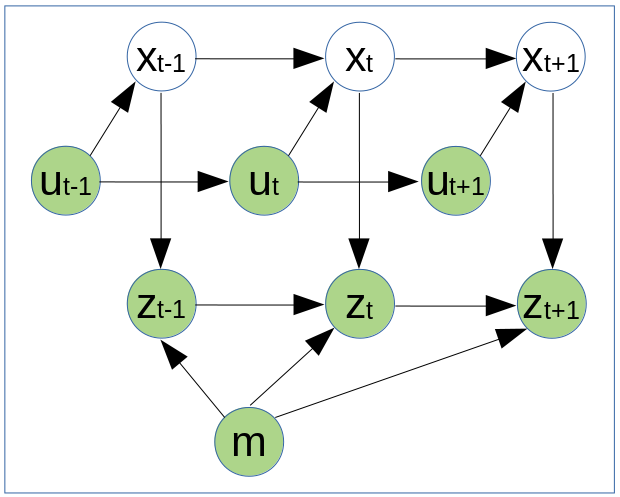
\includegraphics[height=4.0cm]{amcl/location.png}
      \caption{移动机器人定位图例模型}
    \end{figure}
  \end{columns}




  
\end{frame}



\begin{frame}
  \frametitle{定位问题的分类}
  \begin{itemize}
    \item 局部定位与全局定位
    \begin{itemize}
      \item {\color{red}局部定位};也称位姿跟踪,假定机器人初始位姿已知,通过相邻时刻传感器信息对机器人位姿进行跟踪估计。(里程计法、惯性导航法)
      \item {\color{red}全局定位};也称为重定位,机器人初始位姿未知,通过预先确定好的环境模型和传感器信息,计算机器人在全局坐标系中的位姿。(信标定位、地图匹配、GPS)
      \item {\color{red}机器人绑架};是全局定位问题的一个变种,机器人在运行过程中被绑架(瞬间被移动到其他位置)。
            绑架问题比全局定位更困难,因为机器人可能相信知道自己在哪儿,尽管它不在那里。而全局定位,机器人知道不知道自己在哪儿。
    \end{itemize}
    % \item 静态环境与动态环境
    % \item 主动定位与被动定位
    % \item 单机器人与多机器人
  \end{itemize}
  
\end{frame}

\begin{frame}
  \frametitle{定位问题的分类}
  \begin{itemize}
    \item 静态环境定位与动态环境定位
    \begin{itemize}
      \item 静态环境;定位过程中只有机器人在移动,环境里其他目标保持在同一位置。静态环境具有一些很好的数学特性,使得机器人服从高效概率估计。
      \item 动态环境;环境中除了移动的机器人外,还有动态的人、日光(对安装摄像头的机器人)、可移动的物体、门等。动态环境定位比静态环境定位更困难。
    \end{itemize}
    \item 被动定位与主动定位
    \begin{itemize}
      \item 被动定位;定位算法仅观察机器人运动。机器人通过其他方式控制,并且机器人运动不针对便于定位。比如,机器人随意移动或执行它的任务。
      \item 主动定位;定位算法控制机器人运动,以便最小化定位误差。主动定位方法往往能产生比被动定位方法更好的定位结果。
    \end{itemize}
  \end{itemize}
  
\end{frame}

\begin{frame}
  \frametitle{定位问题的分类}
  \begin{itemize}
    \item 单机器人定位与多机器人定位
    \begin{itemize}
      \item 单机器人定位;在单一机器人平台上收集所有数据,执行定位算法,不存在通信问题。
      \item 多机器人定位;机器人能相互探测,共享自身位置及传感器数据,定位有可能做的更好。
    \end{itemize}
  \end{itemize}
\end{frame}


\begin{comment}
1.表示:贝叶斯网、马尔科夫网、因子图
2.推理:精确推理和近似推理
3.参数学习

1.最速下降:负梯度方向搜索,收敛速度慢。
2.Newton法:保留了泰勒展开的一阶和二阶项,二次收敛速度,但每步都需要计算法Hessian矩阵,复杂的高。
3.GN法:通过Jacobian矩阵近似H矩阵,提高了算法的效率,但H矩阵不满秩则无法迭代。
4.LM法:基于信赖域算法,解决H矩阵不满秩或非正定问题。

\end{comment}
\begin{frame}
  \frametitle{定位问题的求解}
  \centering
  \fbox{
  \parbox{0.8\textwidth}{
    \begin{center}
      定位问题求解大致分为两类:滤波方法和优化(图优化)方法。
    \end{center}
    }
  }
  \begin{columns}
    \column{0.5\textwidth}
    \begin{figure}
      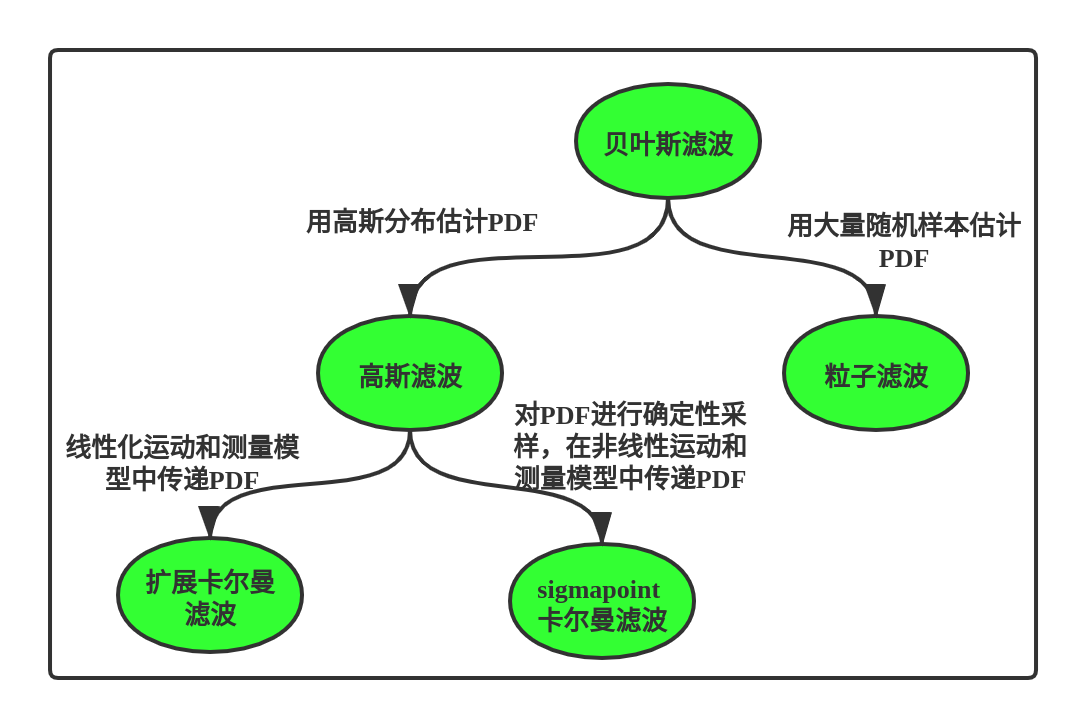
\includegraphics[height=4.0cm]{amcl/filter.png}
      \caption{滤波方法定位}
    \end{figure}
    \column{0.5\textwidth}
    \begin{figure}
      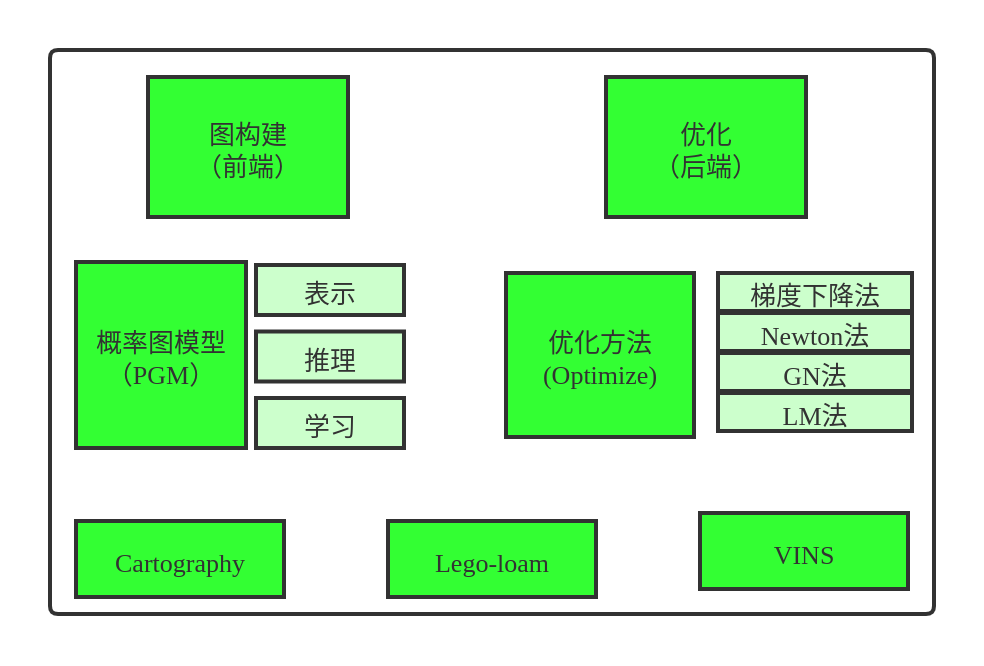
\includegraphics[height=4.0cm]{amcl/optimize.png}
      \caption{图优化方法定位}
    \end{figure}
  \end{columns}


\end{frame}




\begin{comment}
蒙特卡罗方法也称统计模拟方法,通过采样来获得目标分布。从而将数值计算问题转化为概率统计的方法。
MCMC是很多算法求解的基础,在机器学习和强化学习都有广泛的应用

MC:解决难以用数值计算的问题转换为概率统计的方法

感知、定位、建图包含很深的理论。

MCMC采样
\end{comment}

\begin{frame}
  \frametitle{自适应蒙特卡罗定位(AMCL)}
  \begin{columns}
    \column{0.5\textwidth}
    \begin{itemize}
      \item 蒙特卡罗方法(MC):也称统计模拟方法,通过采样来获得目标分布,采样方式包括了{\color{red}概率分布采样}、接受-拒接采样和Gibbs采样等。
      \item 蒙特卡洛定位(MCL):是一种用粒子表示机器人位姿置信度$bel(x_t)$的定位算法。
    \end{itemize}
    \column{0.5\textwidth}
    \begin{figure}
      \includegraphics[width=3.5cm]{amcl/mcl.png}
      \caption{MCL算法流程}
    \end{figure}
  \end{columns}

\end{frame}

\begin{comment}
1.这里介绍一种能够实现自动调节粒子数量的算法-库尔贝克-莱布勒散度。

2.熵:

如果对深度学习有了解的话,深度学习的损失函数中有一个交叉熵的概念。
!!交叉熵是深度学习中常用的一个概念。用在损失函数中求目标与预测值之间的差距。
信息论:熵--信息量,
信息量应该和事件发生的概率有关; $I(x_0) = -\log(p(x_0))$
当越不可能的事件发生了,我们获取到的信息量就越大;
!!熵用来表示所有信息量的期望; $H(X) = - \sum_{i=1}^n p(x_i)\log(p(x_i))$

3 相对熵(KL散度)
对于同一个随机变量 x 有两个单独的概率分布 P(x) 和 Q(x),
我们可以使用 KL 散度(Kullback-Leibler (KL) divergence)来衡量这两个分布的差异

\end{comment}

\begin{frame}
  \frametitle{自适应蒙特卡罗定位(AMCL)}
  \begin{itemize}
    \item 对于粒子滤波器的效率来说,用于表示置信度采样集的大小是一个重要的参数。在定位的早期阶段高的粒子数可能是定位所必须的,
          但是一旦知道机器人在哪里,仅需要一小部分粒子就足以跟踪机器人的位姿。
    \item {\color{red}库尔贝克-莱布勒散度}(Kullback-Leiber Divergence,KLD),也称为相对熵(relative entropy),是描述两个概率分布P和Q差异的一种方法。
          在信息论中,$D(P||Q)$表示当用概率分布Q来拟合真实分布P时,产生的信息损耗。
    \item 对于一个离散随机变量的两个概率分布P和Q来说,他们的KL散度定义为:
          $$D(P||Q) = 
          \sum_{i=1}^N p(x_i) \cdot \log \frac{p(x_i)}{q(x_i)} = 
          \sum_{i=1}^N p(x_i) \log(p(x_i)) - \sum_{i=1}^N p(x_i)\log(q(x_i))$$
  \end{itemize}
  
\end{frame}

\begin{frame}
  \frametitle{AMCL算法}

  \begin{columns}
    \column{0.1\textwidth}
    \column{0.8\textwidth}
    \begin{block}
      
    \begin{algorithmic}[1]

      \State Algorithm AMCL$(\mathcal{X}_{t-1}, u_t, z_t, m, \epsilon, \sigma)$
      \State $\mathcal{X}_t = \emptyset, M = 0, M_{\mathcal{X}} = 0, k = 0$
      \State for all b in H do  
      \State \quad $b = empty$
      % \State endfor
      \State do
      \State \quad draw i with probability $\propto w_{t-1}^{[i]}$
      \State \quad $x_t^{[M]} = \text{sample\_motion\_model}(u_t, x_{x-1}^{[i]})$
      \State \quad $w_t^{[M]} = \text{measurement\_model}(z_t, x_t^{[M]}, m)$
      \State \quad $\mathcal{X}_t = \mathcal{X}_t + \left\langle x_t^{[M]}, w_t^{[M]} \right \rangle$
    \end{algorithmic}
    \end{block}

    \column{0.1\textwidth}
  \end{columns}
\end{frame}

\begin{frame}
  \frametitle{AMCL算法}

  \begin{columns}
    \column{0.1\textwidth}
    \column{0.8\textwidth}
    \begin{block}
      
    \begin{algorithmic}[1]

      \State \quad $\text{if } x_t^{[M]} \text{ falls in empty bin b then}$  \textit{
        \tiny // 如果新产生的粒子落入直方图的一个空位里} %\textbf{//}
      \State \qquad $k = k+1$ 
      \State \qquad $b = \text{non-empty}$
      \State \qquad $\text{if } k > 1 \text{ then}$ \textit{\tiny  // 粒子越分散,越多的空位被填满,计算得到$M_{\mathcal{X}}$就越大}
      \State \qquad \quad $M_{\mathcal{X}} := \frac{k-1}{2\epsilon} \left\{1 - \frac{2}{9(k-1)} + \sqrt{\frac{2}{9(k-1)}}z_{1-\sigma} \right\} ^3$
      \State \qquad $M = M + 1$
      \State $\text{while } M < M_{\mathcal{X}} \ or \ M < M_{\mathcal{X}min}$
      \State return $X_t$
    \end{algorithmic}
    \end{block}

    \column{0.1\textwidth}
  \end{columns}
\end{frame}

% \text{}
% {\color{Blue} aa}
% \begin{frame}
%   \frametitle{AMCL算法}

%   \begin{columns}
%     \column{0.1\textwidth}
%     \column{0.8\textwidth}
%     \begin{block} 
%     \begin{algorithmic}[1]

%       % \State \quad $\text{if } x_t^{[M]} \text{ falls in empty bin b then} $ \sum
%       % \State \quad $x_t^{[M]} = \text{sample\_motion\_model}(u_t, x_{x-1}^{[i]})$
%       % \State \quad $w_t^{[M]} = \text{measurement\_model}(z_t, x_t^{[M]}, m)$
%       % \State \quad $\mathcal{X}_t = \mathcal{X}_t + \left\langle x_t^{[M]}, w_t^{[M]} \right \rangle$
%     \end{algorithmic}
%     \end{block}

%     \column{0.1\textwidth}
%   \end{columns}
% \end{frame}

% \begin{frame}
%   \frametitle{定位问题概念}
%   \begin{itemize}
%     \item 
%   \end{itemize}
  
% \end{frame}


%\section{AMCL中odometry的数据处理}



\begin{frame}{AMCL中odom部分参数配置}
  AMCL关于odom的参数配置列表(以差速模型为例):

  % \frametitle{表格}
  \begin{table}[htbp!]
    \centering
    % \caption{}
    \begin{tabular}{c|c|c}
      \toprule[1pt]
      参数	& 默认值 & 描述  \\
      \toprule[1pt]
      odom\_model\_type	& diff & 里程计运动模型,种类有diff、ommi等 \\
 	    \hline
      odom\_alpha1	&  0.2 & 机器人旋转分量中的旋转噪声 \\
      \hline
      odom\_alpha2	&  0.2 & 机器人平移分量中的旋转噪声 \\
      \hline
      odom\_alpha3	&  0.2 & 机器人平移分量中的平移噪声 \\
      \hline
      odom\_alpha4	&  0.2 & 机器人旋转分量中的平移噪声 \\
 	    \bottomrule[1pt]
    \end{tabular}
  \end{table}
\end{frame}

% \begin{frame}
%   \frametitle{里程计运动模型(一)}
%   \begin{itemize}
%     \item 在计算时间$\Delta t$内,控制$u_t = (\nu, \omega)$ 作用下将机器人位姿从$x_{t-1} = (x, y, z)^T$ 
%           变成位姿$x_t = (x^\prime, y^\prime, \theta^\prime)^T$ 的概率$p(x_t | u_t, x_{t-1})$ 。
%     \item 为了保持状态空间比较小,通常把里程计数据认为是控制信号。
%     \item 总之,用距离测量代替控制, 距离是通过里程计编码信息得到的。
%   \end{itemize}

% \end{frame}


  \begin{frame}{里程计运动模型}
    
    \begin{columns}%0.6 0.4表示相对比例
    \column{0.5\textwidth}%<1->
    % \frametitle{条目}
    \begin{itemize}
    \item 里程计差分模型:两平行轮作驱动,另外附加一个万向轮作支撑。
    \item 在AMCL算法中将机器人的每一步的广义运动进行了拆解,拆解成包含三个动作的序列:
      \begin{itemize}
        \item 在起始点旋转,转向终止点的方向
         \item 朝着该方向做直线运动到终止点
         \item 在终止点进行旋转,转到目标方向
      \end{itemize}

    \end{itemize}

    \column{0.5\textwidth}%<1->
    % 分栏的右侧插入了图片。
     \begin{figure}[!h]
      \centering
      % Requires \usepackage{graphicx}
      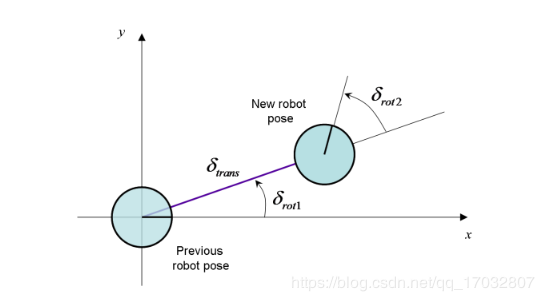
\includegraphics[width=5cm,trim=50 25 50 50,clip]{amcl/odom_model}\\
      % \caption{logo图片样例}\label{pic6}
    \end{figure}
    \begin{itemize}
      \item $\delta_{rot1}$代表在起始点的旋转
      \item $\delta_{trans}$代表着第二段平移过程
      \item $\delta_{rot2}$代表着在终止点的旋转
    \end{itemize}
    \end{columns}
    % 分栏后面的一些内容!!
    \end{frame}

\begin{frame}{里程计运动模型的噪声}
  % \begin{itemize}
	% 	\item 在起始点旋转,转向终止点的方向
	%  	\item 着该方向做直线运动到终止点
	%  	\item 在终止点进行旋转,转到目标方向
  %  \end{itemize}
  \begin{itemize}
  \item 里程计无噪声情况: 里程计读轮子的转圈和机器人的位移是精确对应的。
  \item   理论和仿真可以做到,假设:
    \begin{itemize}
      \item 轮子与地面不打滑
      \item 地面绝对平整
      \item 轮子不变形
      \item 里程计和机器人轮轴之间没有迟滞可以做到完全时间同步,等等
    \end{itemize}
  \item 在AMCL中,里程计是作为{\color{red}状态预测器}存在的,根据控制信息和上一时刻机器人的状态,同时考虑里程计噪声信息,对当前时刻状态进行预测。
  \end{itemize}
\end{frame}  

\begin{frame}
  \frametitle{概率分布采样}

  {\color{red}Box-Muller变换}是通过服从均匀分布的随机变量,来构建服从高斯分布的随机变量的一种方法。
  具体的描述为:选取两个服从[0,1]上均匀分布的随机变$x_1$, $x_2$, $y_1$, $y_2$满足:

  \begin{equation}
    \begin{cases}
      y_1 = \frac{x_1}{\sqrt{w}} \sqrt{-2 \ln{w}} \\
      y_2 = \frac{x_2}{\sqrt{w}} \sqrt{-2 \ln{w}}
    \end{cases}
  \end{equation}

  其中,$w = x_1^2 + x_2^2$,$y_1$和$y_2$是服从$N(0,1)$分布的随机数;

  % 代码实现里面取的是$y_2$,并且在$y_2$前面乘以sigma,获得N(0, sigma)分布的随机数。

\end{frame}


\begin{comment}
1.算法将初始位姿和里程计读数作为输入;
2.运动模型的三个动作序列
\end{comment}
\begin{frame}[fragile]
  \frametitle{运动模型采样算法}

    \begin{columns}
      \column{0.1\textwidth}
      \column{0.8\textwidth}
    \begin{block}
      
    
    \begin{algorithmic}[1]
        \State Algorithm sample\_motion\_model\_odometry$(u_t, x_{t-1})$ :
        \State $\delta_{rot1} = atan2(\delta_x, \delta_y) - \theta_{old}$
        \State $\delta_{trans} = \sqrt{\delta_x^2 + \delta_y^2}$
        \State $\delta_{rot2} = \delta_\theta - \delta_{rot1}^2$

        \State $\hat{\delta}_{rot1} = \delta_{rot1} - smaple(\alpha_1 \delta_{rot1}^2 + \alpha_2 \delta_{trans}^2)$
        \State $\hat{\delta}_{trans} = \delta_{trans} - smaple(\alpha_3 \delta_{trans}^2 + \alpha_4 \delta_{rot1}^2 + \alpha_4 \delta_{rot2}^2)$
        \State $\hat{\delta}_{rot2} = \delta_{rot2} - smaple(\alpha_1 \delta_{rot2}^2 + \alpha_2 \delta_{trans}^2)$

        \State $x^\prime = x + \hat{\delta}_{trans} \cos(\theta + \hat{\delta}_{rot1})$
        \State $y^\prime = y + \hat{\delta}_{trans} \sin(\theta + \hat{\delta}_{rot1})$
        \State $\theta^\prime = \theta + \hat{\delta}_{rot1}  + \hat{\delta}_{rot2}$

        \State return $x_t = (x^\prime, y^\prime, \theta^\prime)^T$

    \end{algorithmic}
  \end{block}

  \column{0.1\textwidth}

  \end{columns}
  % \end{algorithm}

\end{frame}






\begin{comment}
旋转分量中的旋转噪声;
平移分量中的旋转噪声;
平移分量中的平移噪声;
旋转分量中的平移噪声;
1.
\end{comment}

\begin{frame}[fragile]
  \frametitle{Odom代码分析}

  % 入口函数:

  % \begin{lstlisting}[frame=shadowbox]
  %   bool AMCLOdom::UpdateAction(pf_t *pf, AMCLSensroData *data);
  % \end{lstlisting}

  % 计算 $\delta_{rot1}$、$\delta _{rot2}$和$\delta _{trans}$:
  \begin{lstlisting}[frame=shadowbox]
    bool AMCLOdom::UpdateAction(pf_t *pf, AMCLSensroData *data)
    {
      ndata = (AMCLOdomData*) data;

      if (sqrt(ndata->delta.v[0]*ndata->delta.v[0] + ndata->delta.v[1]*ndata->delta.v[1]) < 0.01) 
        delta_rot1 = 0.0;
      else
        delta_rot1 = angle_diff(atan2(ndata->delta.v[1], ndata->delta.v[0]), old_pose.v[2]);

      delta_trans = sqrt(ndata->delta.v[0]*ndata->delta.v[0] + ndata->delta.v[1]*ndata->delta.v[1]);
      delta_rot2 = angle_diff(ndata->delta.v[2], delta_rot1);
  \end{lstlisting}


\end{frame}


\begin{frame}[fragile]
  \frametitle{Odom代码分析}
  \begin{lstlisting}[frame=shadowbox]
      delta_rot1_noise = std::min(fabs(angle_diff(delta_rot1, 0.0)), fabs(angle_diff(delta_rot1, M_PI)));
      delta_rot2_noise = std::min(fabs(angle_diff(delta_rot2, 0.0)), fabs(angle_diff(delta_rot2, M_PI)));

      for(int i=0; i<set->sample_count; i++)
      {
        pf_sample_t* sample = set->samples + i;
        delta_rot1_hat = angle_diff(delta_rot1, pf_ran_gaussian(alpha1_*delta_rot1_noise*delta_rot1_noise + alpha2_*delta_trans*delta_trans));
        delta_rot2_hat = angle_diff(delta_rot2, pf_ran_gaussian(alpha1_*delta_rot2_noise*delta_rot2_noise + alpha2_*delta_trans*delta_trans));
        delta_trans_hat = delta_trans - pf_ran_gaussian(alpha3_*delta_trans*delta_trans + alpha4_*delta_rot1_noise*delta_rot1_noise + alpha5_*delta_rot2_noise*delta_rot2_noise);
  \end{lstlisting}
\end{frame}

\begin{frame}[fragile]
  \frametitle{Odom代码分析}
  \begin{lstlisting}[frame=shadowbox]
        sample->pose.v[0] += delta_trans_hat * cos(sample->pose.v[2] + delta_rot1_hat);  
        sample->pose.v[1] += delta_trans_hat * sin(sample->pose.v[2] + delta_rot1_hat);  
        sample->pose.v[2] += delta_rot1_hat + delta_rot2_hat;
      }
    }
  \end{lstlisting}
  % \ref{pf_ran_gaussian}
\end{frame}

\begin{frame}[fragile]
  \frametitle{Odom代码分析}
  \label{pf_ran_gaussian}
  \begin{lstlisting}[frame=shadowbox]  
    double pf_ran_gaussian(double sigma)
    {
      double x1, x2, w, r;
      do
      {
        do { r = drand48(); } while (r==0.0);
        x1 = 2.0 * r - 1.0;
        do { r = drand48(); } while (r==0.0);
        x2 = 2.0 * r - 1.0;
        w = x1*x1 + x2*x2;
      } while(w > 1.0 || w==0.0);
      return(sigma * x2 * sqrt(-2.0*log(w)/w));
    }
  \end{lstlisting}
\end{frame}
%\section{AMCL中laser的数据处理}

% \subsection{}

\begin{frame}
  \frametitle{AMCL中laser部分参数配置}
  % 
  
  \begin{table}[htbp!]
    \centering
    % \caption{}
    % \setlength{\tabcolsep}{2mm}{
    \resizebox{\textwidth}{25mm}{
    \begin{tabular}{c|c|c}
      % \begin{tabular}{p{2cm}|p{2cm}|p{5cm}}
      \toprule[1pt]
      参数	& 默认值 & 描述  \\
      \toprule[1pt]
      laser\_min\_range	& -1.0 & 考虑的最小扫描范围;参数设置为 -1.0时,将会使用激光上报的最小扫描范围 \\
 	    \hline
       laser\_max\_range	&  -1.0 & 考虑的最大扫描范围;参数设置为-1.0时,将会使用激光上报的最大扫描范围 \\
      \hline
      laser\_max\_beams	&  180 & 更新滤波器时,每次扫描中多少个光束被使用 \\
      \hline
      laser\_model\_type	&  likehood\_field & 模型使用,可以是beam, likehood\_field, likehood\_field\_prob \\
      \hline
      laser\_z\_hit	&  0.95 & 测量点到对应物体之间的距离的误差所占最终计算得到的距离的权重 \\
      \hline
      laser\_z\_rand	&  0.05 & 随机噪声的权重 \\
      \hline
      laser\_sigma\_hit	&  0.2 & 被用在模型的z\_hit部分的高斯模型的标准差 \\
      \hline
      laser\_likelihood\_max\_dist	&  0.325 & 似然域预处理设置的最大距离 \\
 	    \bottomrule[1pt]
    \end{tabular}}
  \end{table}

\end{frame}

\begin{frame}
  \frametitle{激光的波束模型---简介}
  \begin{itemize}
    \item 激光传感器测量到附近物体的距离,沿着一个波束测量距离。
    \item 波束模型采用四类测量误差,包括:{\color{red}局部测量噪声}、{\color{red}意外对象引起的误差}、{\color{red}未检测到对象引起的误差}
    和{\color{red}随机意外噪声}。
    \item 波束模型期望概率$p(z_t | x_t, m)$是四类误差分布的混合,每种分布都与一个特定类型的误差有关。
  \end{itemize}
  

\end{frame}

\begin{frame}
  \frametitle{激光的波束模型---局部测量噪声}
  
  \begin{itemize}
    \item 在一个理想世界中,测距仪总是测量位于其测量领域内的最近物体的正确距离。
    \item 现实中,{\color{red}传感器存在有限分辨率及大气对测量信号等影响因素}。
    \item 这个测量噪声通常由一个窄的均值为$z_t^{k*}$、标准偏差为$\sigma_{hit}$的高斯分布建模,如式\ref{eq:laser_celiang}所示。
  \end{itemize}

  \begin{equation}
    p_{short}(z_t^k | x_t, m) = 
    \begin{cases}
      \eta \mathcal{N}(z_t^k; z_t^{k*}, \sigma_{hit}^2) \quad  0 \leq z_t^k \leq z_{max}\\
      0 \qquad \qquad \qquad \quad others
    \end{cases}
    \label{eq:laser_celiang}
  \end{equation}
  

\end{frame}

\begin{frame}
  \frametitle{激光的波束模型---意外对象}
  \begin{itemize}
    \item 移动机器人的环境是动态的,而地图$m$是静态的。
    \item {\color{red}典型的移动对象就是与机器人共享操作空间的人}。
    \item 如果将这类对象作为传感器的噪声来处理,未建模对象具有这样的特性,即它们会导致比$z_t^{k*}$更短而不是更长的距离,并且检测到未建模对象的
          可能性随着距离增大而较少。
    \item 这种情况下距离测量的概率在数学上用一个指数分布来描述,如式\ref{eq:laser_yiwai}所示。
  \end{itemize}

  \begin{equation}
    p_{short}(z_t^k | x_t, m) = 
    \begin{cases}
      \eta \lambda_{short} e^{-\lambda_{short} z_t^k} \quad  0 \leq z_t^k \leq z_t^{k*}\\
      0 \qquad \qquad \qquad \quad others
    \end{cases}
    \label{eq:laser_yiwai}
  \end{equation}
\end{frame}

\begin{frame}
  \frametitle{激光的波束模型---检测失败}
  \begin{itemize}
    \item 有时环境中的噪声会被完全忽略,例如:{\color{red}激光测距仪检测到黑色吸光的对象时,或者某些激光系统在明媚阳光下测量物体时,会发生检测失败}。
    \item 传感器检测失败的典型结果是最大距离问题:传感器返回它的最大允许值$z_{max}$
    \item 用一个以$z_{max}$为中心的点群分布来建立这种情况的模型,如式\ref{eq:laser_jiance}所示。
  \end{itemize}

  \begin{equation}
    p_{max}(z_t^k | x_t, m) = I(z_t^{k}=z_{max}) = 
    \begin{cases}
      1 \quad  z_t^{k} = z_{max}\\
      0 \qquad  others
    \end{cases}
    \label{eq:laser_jiance}
  \end{equation}
\end{frame}

\begin{frame}
  \frametitle{激光的波束模型---随机检测}
  \begin{itemize}
    \item 测距仪偶尔会产生完全无法解释的测量,例如,{\color{red}当它们受到不同传感器之间的串扰时}。
    \item 对于这样的测量,将使用一个分布在完整传感器测量范围$[0, z_{max}]$的均匀分布来建立模型, 如式\ref{eq:laser_suiji}所示。
  \end{itemize}

  \begin{equation}
    p_{rand}(z_t^k | x_t, m) = 
    \begin{cases}
      \frac{1}{z_{max}} \quad  0 \leq z_t^k \leq z_{max}\\
      0 \qquad  others
    \end{cases}
    \label{eq:laser_suiji}
  \end{equation}
\end{frame}

\begin{frame}
  \frametitle{激光的波束模型---误差混合}
  \begin{itemize}
    \item 以上4种误差分布通过四个参数$z_{hit}$、$z_{short}$、$z_{max}$、$z_{rand}$进行加权平均混合,
          并且$z_{hit} + z_{short} + z_{max} + z_{rand} = 1$,如式\ref{eq:laser_hunhe}所示。
  \end{itemize}

  \begin{equation}
    p(z_t^k | x_t, m) = 
    \begin{pmatrix}
      z_{hit} \\ z_{short} \\ z_{max} \\ z_{rand}
    \end{pmatrix}
    \cdot 
    \begin{pmatrix}
      p_{hit}(z_t^k | x_t, m) \\p_{short}(z_t^k | x_t, m) \\ p_{max}(z_t^k | x_t, m) \\ p_{rand}(z_t^k | x_t, m)
    \end{pmatrix}
    \label{eq:laser_hunhe}
  \end{equation}
\end{frame}

\begin{frame}[fragile]
  \frametitle{激光的波束模型算法}
  % \begin{center}
  % \begin{block}
  %   \begin{algorithmic}[1]
  %     \State Algorithm beam\_modle$(z_t, x_t, m)$:
  %     \State q = 1
  %   \end{algorithmic}
  % \end{block}
  % \end{center}

  \begin{columns}%0.6 0.4表示相对比例
    \column{0.1\textwidth}%<1->
    \column{0.8\textwidth}%<1->
  \begin{block}
    
    \begin{algorithmic}[1]
        \State Algorithm beam\_modle$(z_t, x_t, m)$:
        \State $q = 1$
        \For{$k=1$ \text{to} $K$ }
        \State compute $z_t^{k*}$ for the measurement $z_k^k$ using ray casting 
        \State $p = z_{hit} \cdot p_{hit}(z_t^k|x_t, m) + z_{short} \cdot p_{short}(z_t^k|x_t, m) + $
        \Statex     \qquad\quad       $z_{max} \cdot p_{max}(z_t^k|x_t, m) + z_{rand} \cdot p_{rand}(z_t^k|x_t, m)$
        \State $q = q \cdot p$
        \EndFor

        \State return $q$

    \end{algorithmic}
  \end{block}
  \column{0.1\textwidth}%<1->
\end{columns}
\end{frame}

\begin{comment}
1.爬山算法是一种简单的贪心搜索算法,该算法每次从当前解的临近解空间中选择一个最优解作为当前解,直到达到一个局部最优解。
  爬山算法实现很简单,其主要缺点是会陷入局部最优解
\end{comment}

\begin{frame}
  \frametitle{激光的波束模型---存在不足}
  \begin{enumerate}
    \item 基于波束的模型表现出{\color{red}缺乏光滑性},在有许多小障碍物的混乱环境中,测量模型$p(x_t^k|x_t, m)$会在$x_t$处高度不连续。
    缺乏光滑性有两个后果:一是任何近似置信度表示法都存在错过正确状态的风险,因为临近的状态可能具有截然不同的后验似然。
    二是不光滑的模型中存在大量的局部极值,用爬坡算法找到的解很可能是局部最优。
    \item 基于波束的模型存在{\color{red}计算量大问题},对传感器每一个测量$z_t^k$的评估$p(z_t^k|x_t, m)$涉及
    四类噪声的分布估计%射线投影%
    ,这需要很大的计算量。
  \end{enumerate}
\end{frame}
%\begin{frame}
  % \frametitle{激光的似然域模型---简介}
  \frametitle{激光的似然域模型}
  \begin{itemize}
    \item 不必计算相对于任何有意义的传感器物理生成模型的条件概率,计算更高效。
    \item 这种方法在实践中运行效果良好,即使在混乱的空间,得到的后验也更加光滑。
  \end{itemize}
\end{frame}

\begin{frame}
  % \frametitle{激光的似然域模型---算法步骤1}
  \frametitle{激光的似然域模型}
  \begin{itemize}
    \item 首先将传感器扫描的终点$z_t$映射到地图的全局坐标空间。
    \item 机器人在t时刻的位姿为$x_t = (x,y, \theta)^T$,
          传感器的安装位置相对于机器人的中心坐标$(x_{k, sens}, y_{k, sens})^T$,
          激光光束相对于机器人的朝向的角度为$\theta_{k, sens}$,
          激光光束测量到的距离值为$z_t^k$ 。
          激光扫描到的点投影到地图的全局坐标系坐标为$(x_{z_t^k}, y_{z_t^k})^T$,如式\ref{eq:siranquan}所示。
  \end{itemize}

  \begin{eqnarray}
    \begin{pmatrix}
      x_{z_t^k} \\ y_{z_t^k}
    \end{pmatrix}
    = 
    \begin{pmatrix}
      x \\ y
    \end{pmatrix}
    +
    \begin{pmatrix}
      \cos\theta \quad -\sin\theta \\
      \sin \theta \qquad \cos\theta
    \end{pmatrix}
    \begin{pmatrix}
      x_{k, sens} \\ y_{k, sens}
    \end{pmatrix}
    +
    z_t^k
    \begin{pmatrix}
      \cos(\theta + \theta_{k, snes}) \\ \sin(\theta + \theta_{k, sens})
    \end{pmatrix}
    \label{eq:siranquan}
  \end{eqnarray}
\end{frame}

\begin{frame}
  % \frametitle{激光的似然域模型---算法步骤2}
  \frametitle{激光的似然域模型}

  \begin{itemize}
    \item 似然域模型假设存在三种类型噪声和不确定性。即测量噪声$p_{hit}$、测量失败$p_{max}$、无法解释的随机测量$p_{rand}$。

  \end{itemize}

  \begin{enumerate}
    \item 测量噪声$p_{hit}$。由测量过程引起的噪声使用高斯进行建模。用$dist$表示测量坐标$(x_{z_t^k}, z_{z_t^k})$与地图$m$上最近物体之间的欧式距离。
          因此传感器测量概率可以用均值为0的高斯函数表示: $$p_{hit}(z_k^t|x_t, m) = \mathrm{\epsilon}_{\sigma_{hit}}(dist)$$
  \end{enumerate}

  \begin{figure}[htbp]
  %   \centering
  %   \subfigure[酒店服务送机器人]{
  %   \begin{minipage}[t]{0.45\linewidth}
  %   \centering
    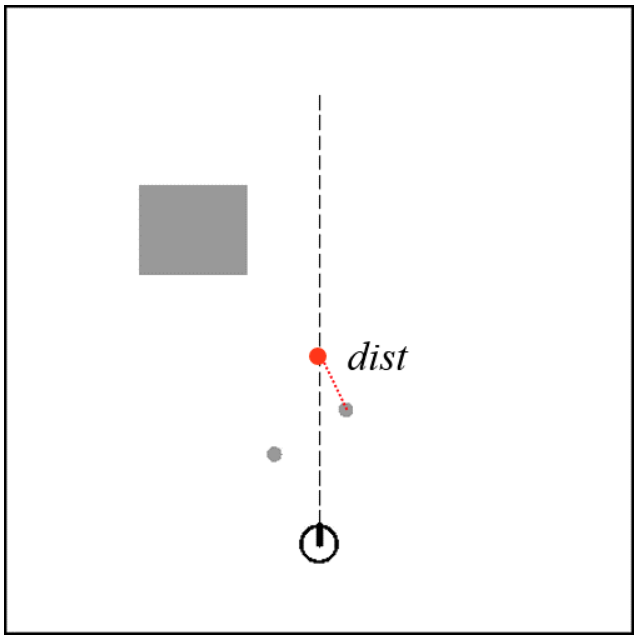
\includegraphics[trim=0mm 0mm 0mm 0mm,clip,height=2.5cm]{amcl/siranyu1}
  %   \label{fig:1gaoxian}
  %   \end{minipage}%
  %   }%
  %   \subfigure[外墙面检查机器人]{
  %   \begin{minipage}[t]{0.45\linewidth}
  %   \centering
    % \includegraphics[trim=0mm 0mm 0mm 0mm,clip,width=5.5cm,height=4.5cm]{1qiangmian}
    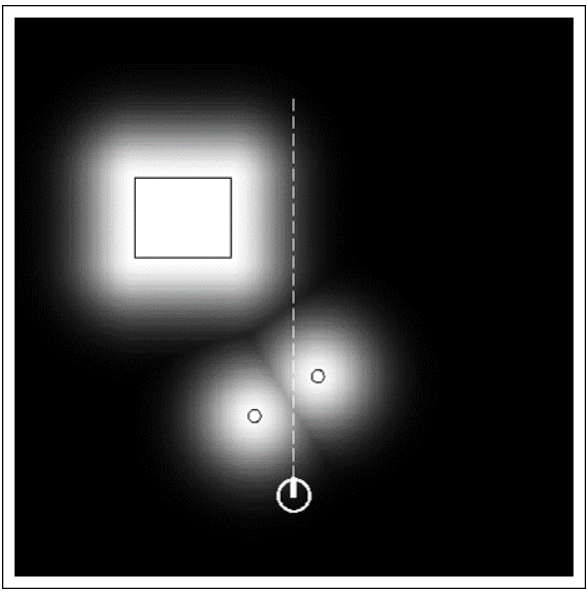
\includegraphics[trim=0mm 0mm 0mm 0mm,clip,height=2.5cm]{amcl/siranyu2}

  %   \label{fig:1qiangmian}
  %   \end{minipage}%
  %   }%
  \end{figure}


\end{frame}

\begin{frame}
  % \frametitle{激光的似然域模型---算法步骤2}
  \frametitle{激光的似然域模型}

  \begin{enumerate}
    \setcounter{enumi}{1}
    \item 测量失败。假定最大距离读数具有非常大的似然值,可用点群分布$p_{max}$进行建模。
    \item 无法解释的随机测量。用一个均匀分布$p_{rand}$描述。
  \end{enumerate}

  \begin{itemize}
    \item 最后,已知$t$时刻位姿$x_t$和地图$m$的情况下,则观测到$z_t^k$的概率$p(z_t^k | x_t, m)$:
          $$p(z_t^k|x_t, m) = z_{hit} \cdot p_{hit} + z_{rand} \cdot p_{rand} + z_{max} \cdot p_{max}$$
          其中$z_{hit}$,$z_{rand}$,$z_{max}$为权重。
  \end{itemize}
  % 最后,已知$t$时刻位姿$x_t$和地图$m$的情况下,则观测到$z_t^k$的概率$p(z_t^k | x_t, m)$:
  %         $$p(z_t^k|x_t, m) = z_{hit} \cdot p{hit} + z_{rand} \cdot p{rand} + z_{max} \cdot p{max}$$
  %         其中$z_{hit}$,$z_{rand}$,$z_{max}$为权重。
\end{frame}

\begin{frame}[fragile]
  % \frametitle{激光的似然域模型---算法}
  \frametitle{激光的似然域模型}

  \begin{columns}
    \column{0.05\textwidth}
    \column{0.9\textwidth}
    \begin{block}

        \begin{algorithmic}[1]
          \State Algorithm likelihood\_field\_model$(z_t, x_t, m)$:
          \State $q = 1$
          \State for all $k$ do
          \State \quad if $z_t^k \neq z_{max}$
          \State \qquad $x_{z_t^k} = x + x_{k, sens} \cos\theta - y_{k, sens} \sin\theta + z_t^k \cos(\theta + \theta_{k, sens})$
          \State \qquad $y_{z_t^k} = y+y_{k, sens}\cos\theta+x_{k, sens}\sin\theta+z_t^k \sin(\theta + \theta_{k, sens})$
          \State \qquad $dist = \substack{\text{min}\\x^\prime, y^\prime} \left\{ \sqrt{(x_{z_t^k}-x^\prime)^2 + (y_{z_t^k} - y^\prime)^2} | \left \langle x^\prime, y^\prime \right \rangle\text{occupied in m} \right\}$
          \State \qquad $q = q \cdot (z_{hit} \cdot prob(dist, \sigma_{hit}) + \frac{z_{random}}{z_{max}})$
          \State return $q$
        \end{algorithmic}
    \end{block}
    \column{0.05\textwidth}
  \end{columns}
\end{frame}

\begin{frame}[fragile]
  \frametitle{代码分析}
  \begin{lstlisting}[frame=shadowbox]  
    //激光雷达位姿变换到全局坐标系下
    pf_vector_t  pf_vector_coord_add(pf_vector_t a, pf_vector_t b) 
    {
      pf_vector_t c;
      c.v[0] = b.v[0] + a.v[0] * cos(b.v[2]) - a.v[1] * sin(b.v[2]);
      c.v[1] = b.v[1] + a.v[0] * sin(b.v[2]) + a.v[1] * cos(b.v[2]);
      c.v[2] = b.v[2] + a.v[2];
      c.v[2] = atan2(sin(c.v[2]), cos(c.v[2]));
      return c;
    }
    ......
    //激光雷达的每个光束末端位置变换到全局坐标系下
    hit.v[0] = pose.v[0] + obs_range * cos(pose.v[2] + obs_bearing); 
    hit.v[1] = pose.v[1] + obs_range * sin(pose.v[2] + obs_bearing);
  \end{lstlisting}
\end{frame}

\begin{frame}[fragile]
  \frametitle{代码分析}
  \begin{lstlisting}
    //计算似然域
    void map_update_cspace(map_t *map, double max_occ_dist)
    {
      unsigned char* marked;
      std::priority_queue<CellData> pq;

      marked = new unsigned char[map->size_x * map->size_y];
      memset(marked, 0, sizeof(unsigned char) * map->size_x * map->size_y);
      map->max_occ_dist = max_occ_dist;

      CachedDistanceMap* cdm = get_distance_map(map->scale, map->max_occ_dist);

      CellData cell;
      cell.map_ = map;
  \end{lstlisting}
\end{frame}

\begin{frame}[fragile]
  \frametitle{代码分析}
  \begin{lstlisting}
      //将地图中表示障碍物栅格push到优先队列中
      for(int i=0; i<map->size_x; i++) {
        cell.src_i_ = cell.i_ = i;
        for(int j=0; j<map->size_y; j++) {
          if(map->cells[MAP_INDEX(map, i, j)].occ_state == +1) {
            map->cells[MAP_INDEX(map, i, j)].occ_dist = 0.0;
            cell.src_j_ = cell.j_ = j;
            marked[MAP_INDEX(map, i, j)] = 1;
            pq.push(cell);
          }
          else 
            map->cells[MAP_INDEX(map, i, j)].occ_dist = max_occ_dist;
        }
      }
  \end{lstlisting}
\end{frame}

\begin{frame}[fragile]
  \frametitle{代码分析}
  \begin{lstlisting}
      //传播算法计算似然域
      while(!pq.empty()) {
        CellData current_cell = pq.top();
        if(current_cell.i_ > 0)
          enqueue(map, current_cell.i_-1, current_cell.j_, current_cell.src_i_, current_cell.src_j_, pq, cdm, marked);
        if((int)current_cell.i_ < map->size_x - 1)
          enqueue(map, current_cell.i_+1, current_cell.j_, current_cell.src_i_, current_cell.src_j_, pq, cdm, marked);
        ......
        pq.pop();
      }
      delete[] marked;
    }
  \end{lstlisting}
\end{frame}

\begin{frame}[fragile]
  \frametitle{代码分析}
  \begin{lstlisting}
    void enqueue(map_t* map, int i, int j, int src_i, int src_j, 
        std::priority_queue<CellData>& pq, CachedDistanceMap* cmd, unsigned char* marked)
    {
      if(marked[MAP_INDEX(map, i, j)]) return;
      int di = abs(i - src_i);
      int dj = abs(j - src_j);
      double distance = cmd->distances_[di][dj];
      if(distance > cmd->cell_radius_) return;
      map->cells[MAP_INDEX(map, i, j)].occ_dist = distance * map->scale;

      CellData cell; cell.map_ = map;
      cell.i_ = i; cell.j_ = j; cell.src_i_ = src_i; cell.src_j_ = src_j;
      pq.push(cell);
      marked[MAP_INDEX(map, i, j)] = 1;
    }
  \end{lstlisting}
\end{frame}

\begin{frame}
  \frametitle{激光的似然域模型的优缺点}
  \begin{itemize}
    \item 优点
    \begin{enumerate}
      \item 光滑性较好,机器人位姿$x_t$的微小改变仅对分布结果$p(z_t^k|x_t,m)$有很小的影响。
      \item 寻找最近障碍物是最耗时的,不过可以通过预计算似然域,搜索时直接查表即可。总的来说该算法较为简单,计算速度也相对较快。
    \end{enumerate}
    \item 缺点
    \begin{enumerate}
      \item 它不能对人或可能引起短读数的其他动态障碍物清晰地建立模型。
      \item 在传感器数据计算障碍点时没有考虑到传感器不能“穿墙”,也就是不能确定到一个点的路径是否被地图上的障碍物所拦截。
      \item 似然域模型没有考虑地图的不确定性,它不能处理地图上不确定或不明确的未探索区域。
    \end{enumerate}
  \end{itemize}
\end{frame}
%\section{小结}

\begin{frame}
  \frametitle{小结}
  \begin{enumerate}
    \item 介绍了机器人定位、分类、方法。
    \item 介绍了AMCL算法
    \item 机器人运动模型和在AMCL中的实现及参数意义
    \item 机器人Lader感知模型和在AMCL中的实现及参数意义
  \end{enumerate}
  
\end{frame}

\begin{frame}
  \frametitle{推荐阅读书籍}
  \begin{columns}
    \column{0.5\textwidth}
    \begin{enumerate}
      \item 《概率机器人》
      \item 《机器人学中的状态估计》
      \item 《视觉SLAM十四讲》
      \item 《概率图模型原理与技术》
      \item 《凸优化》
    \end{enumerate}
    \column{0.5\textwidth}
    \begin{figure}
      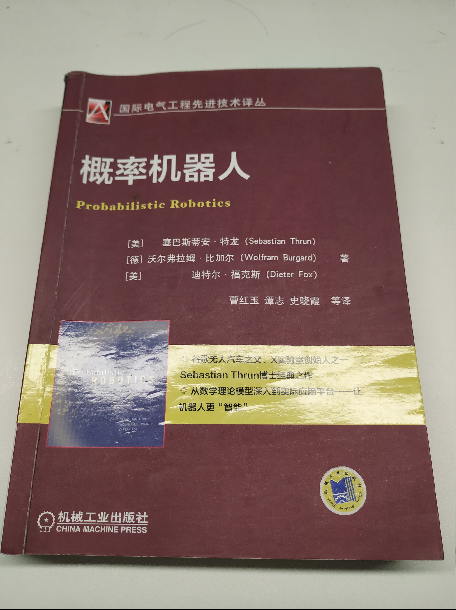
\includegraphics[height=2.5cm]{amcl/refbook1.png}
      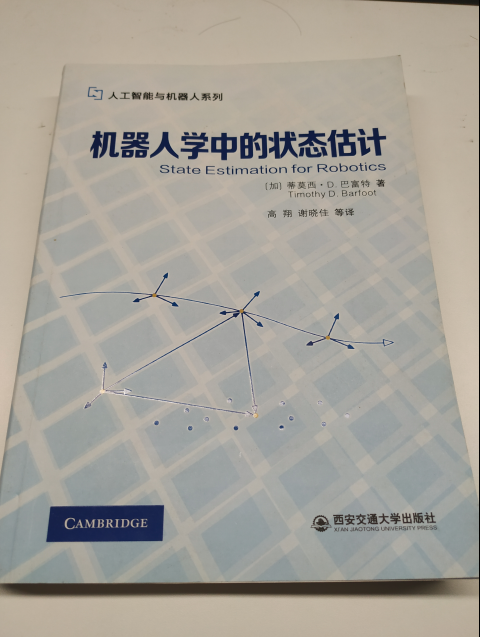
\includegraphics[height=2.5cm]{amcl/refbook2.png}
      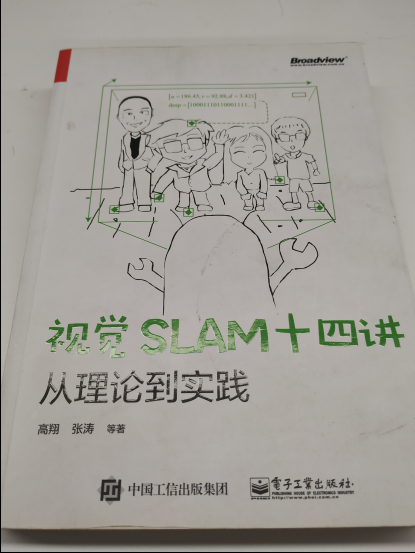
\includegraphics[height=2.5cm]{amcl/refbook4.png}

      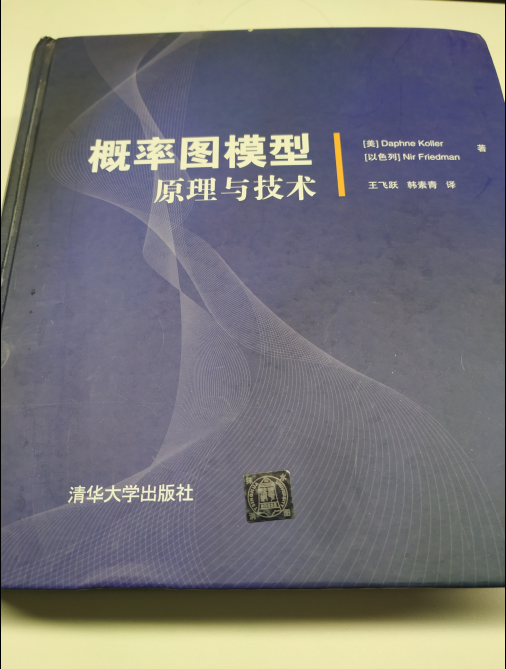
\includegraphics[height=2.5cm]{amcl/refbook3.png}
      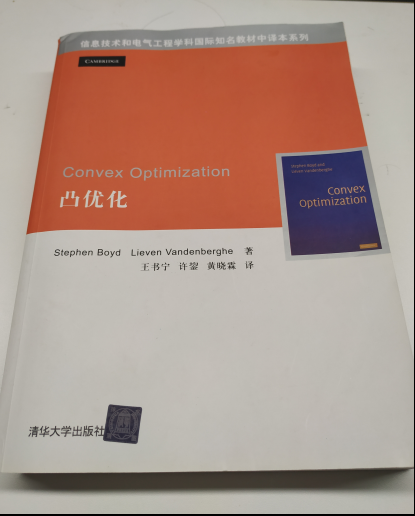
\includegraphics[height=2.5cm]{amcl/refbook5.png}
    \end{figure}
  \end{columns}

  
\end{frame}

% \begin{frame}
%   \begin{figure}
%     % 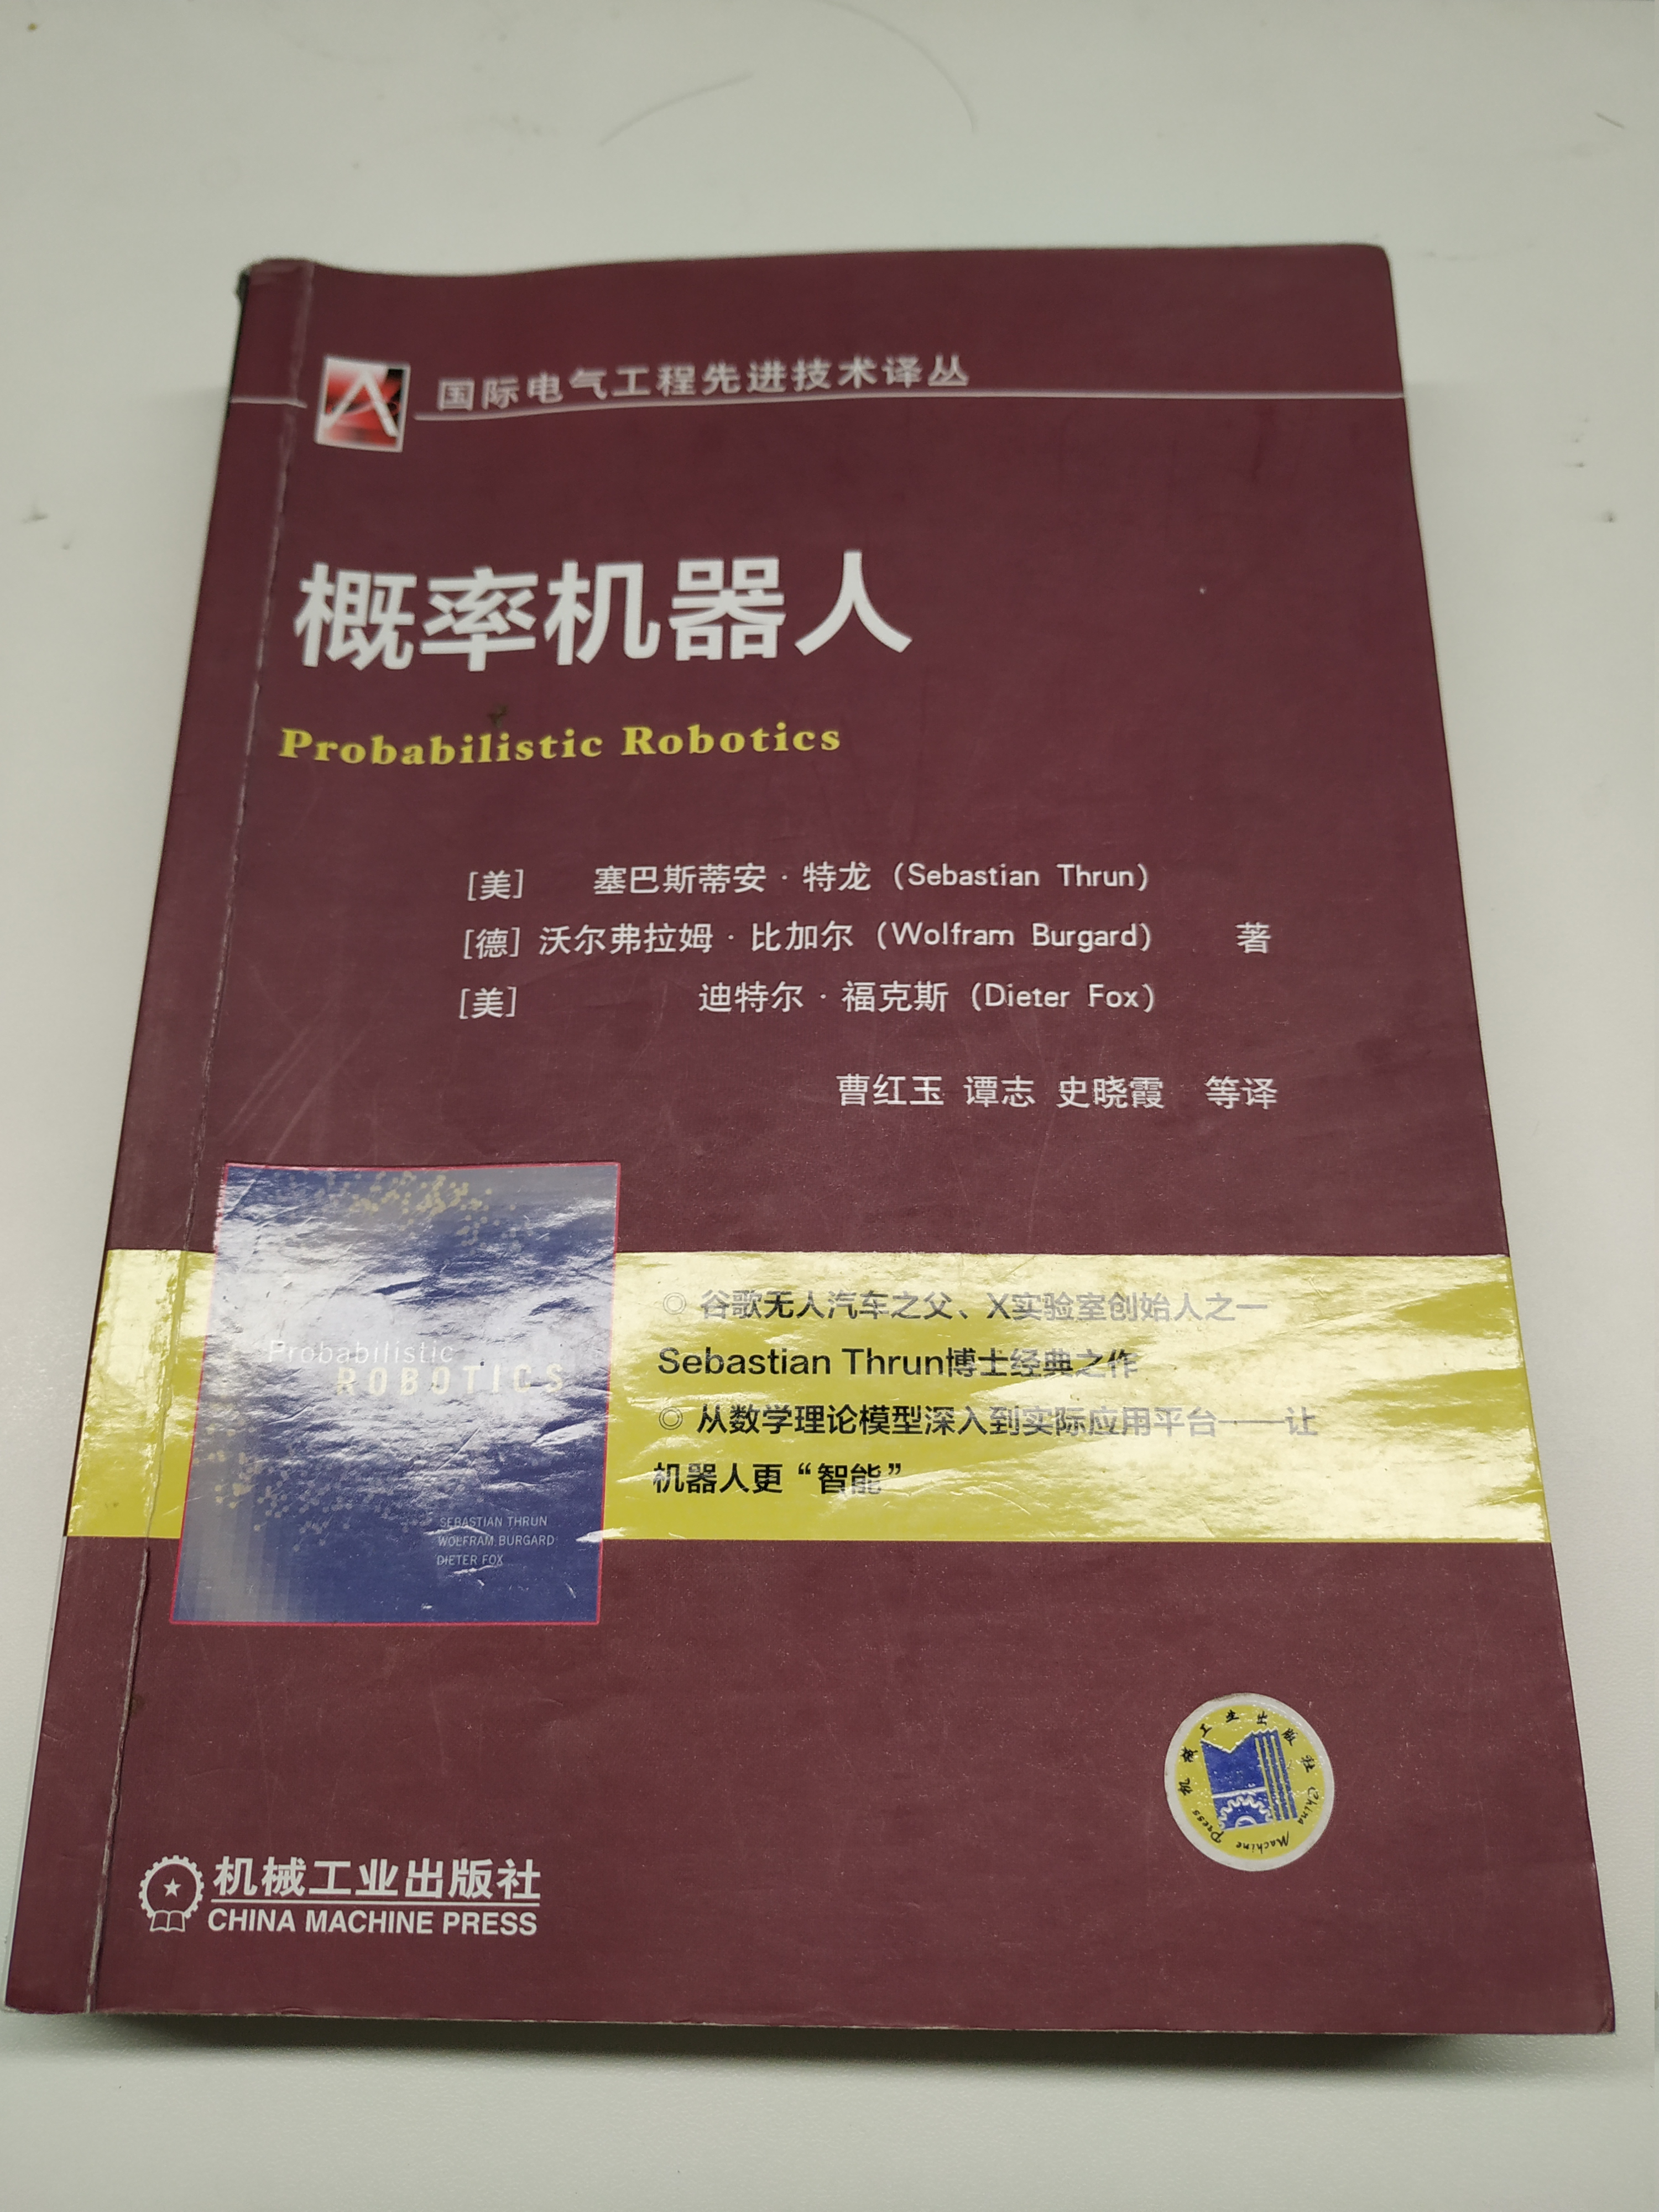
\includegraphics[height=3.0cm]{amcl/gljqr.jpg}
%     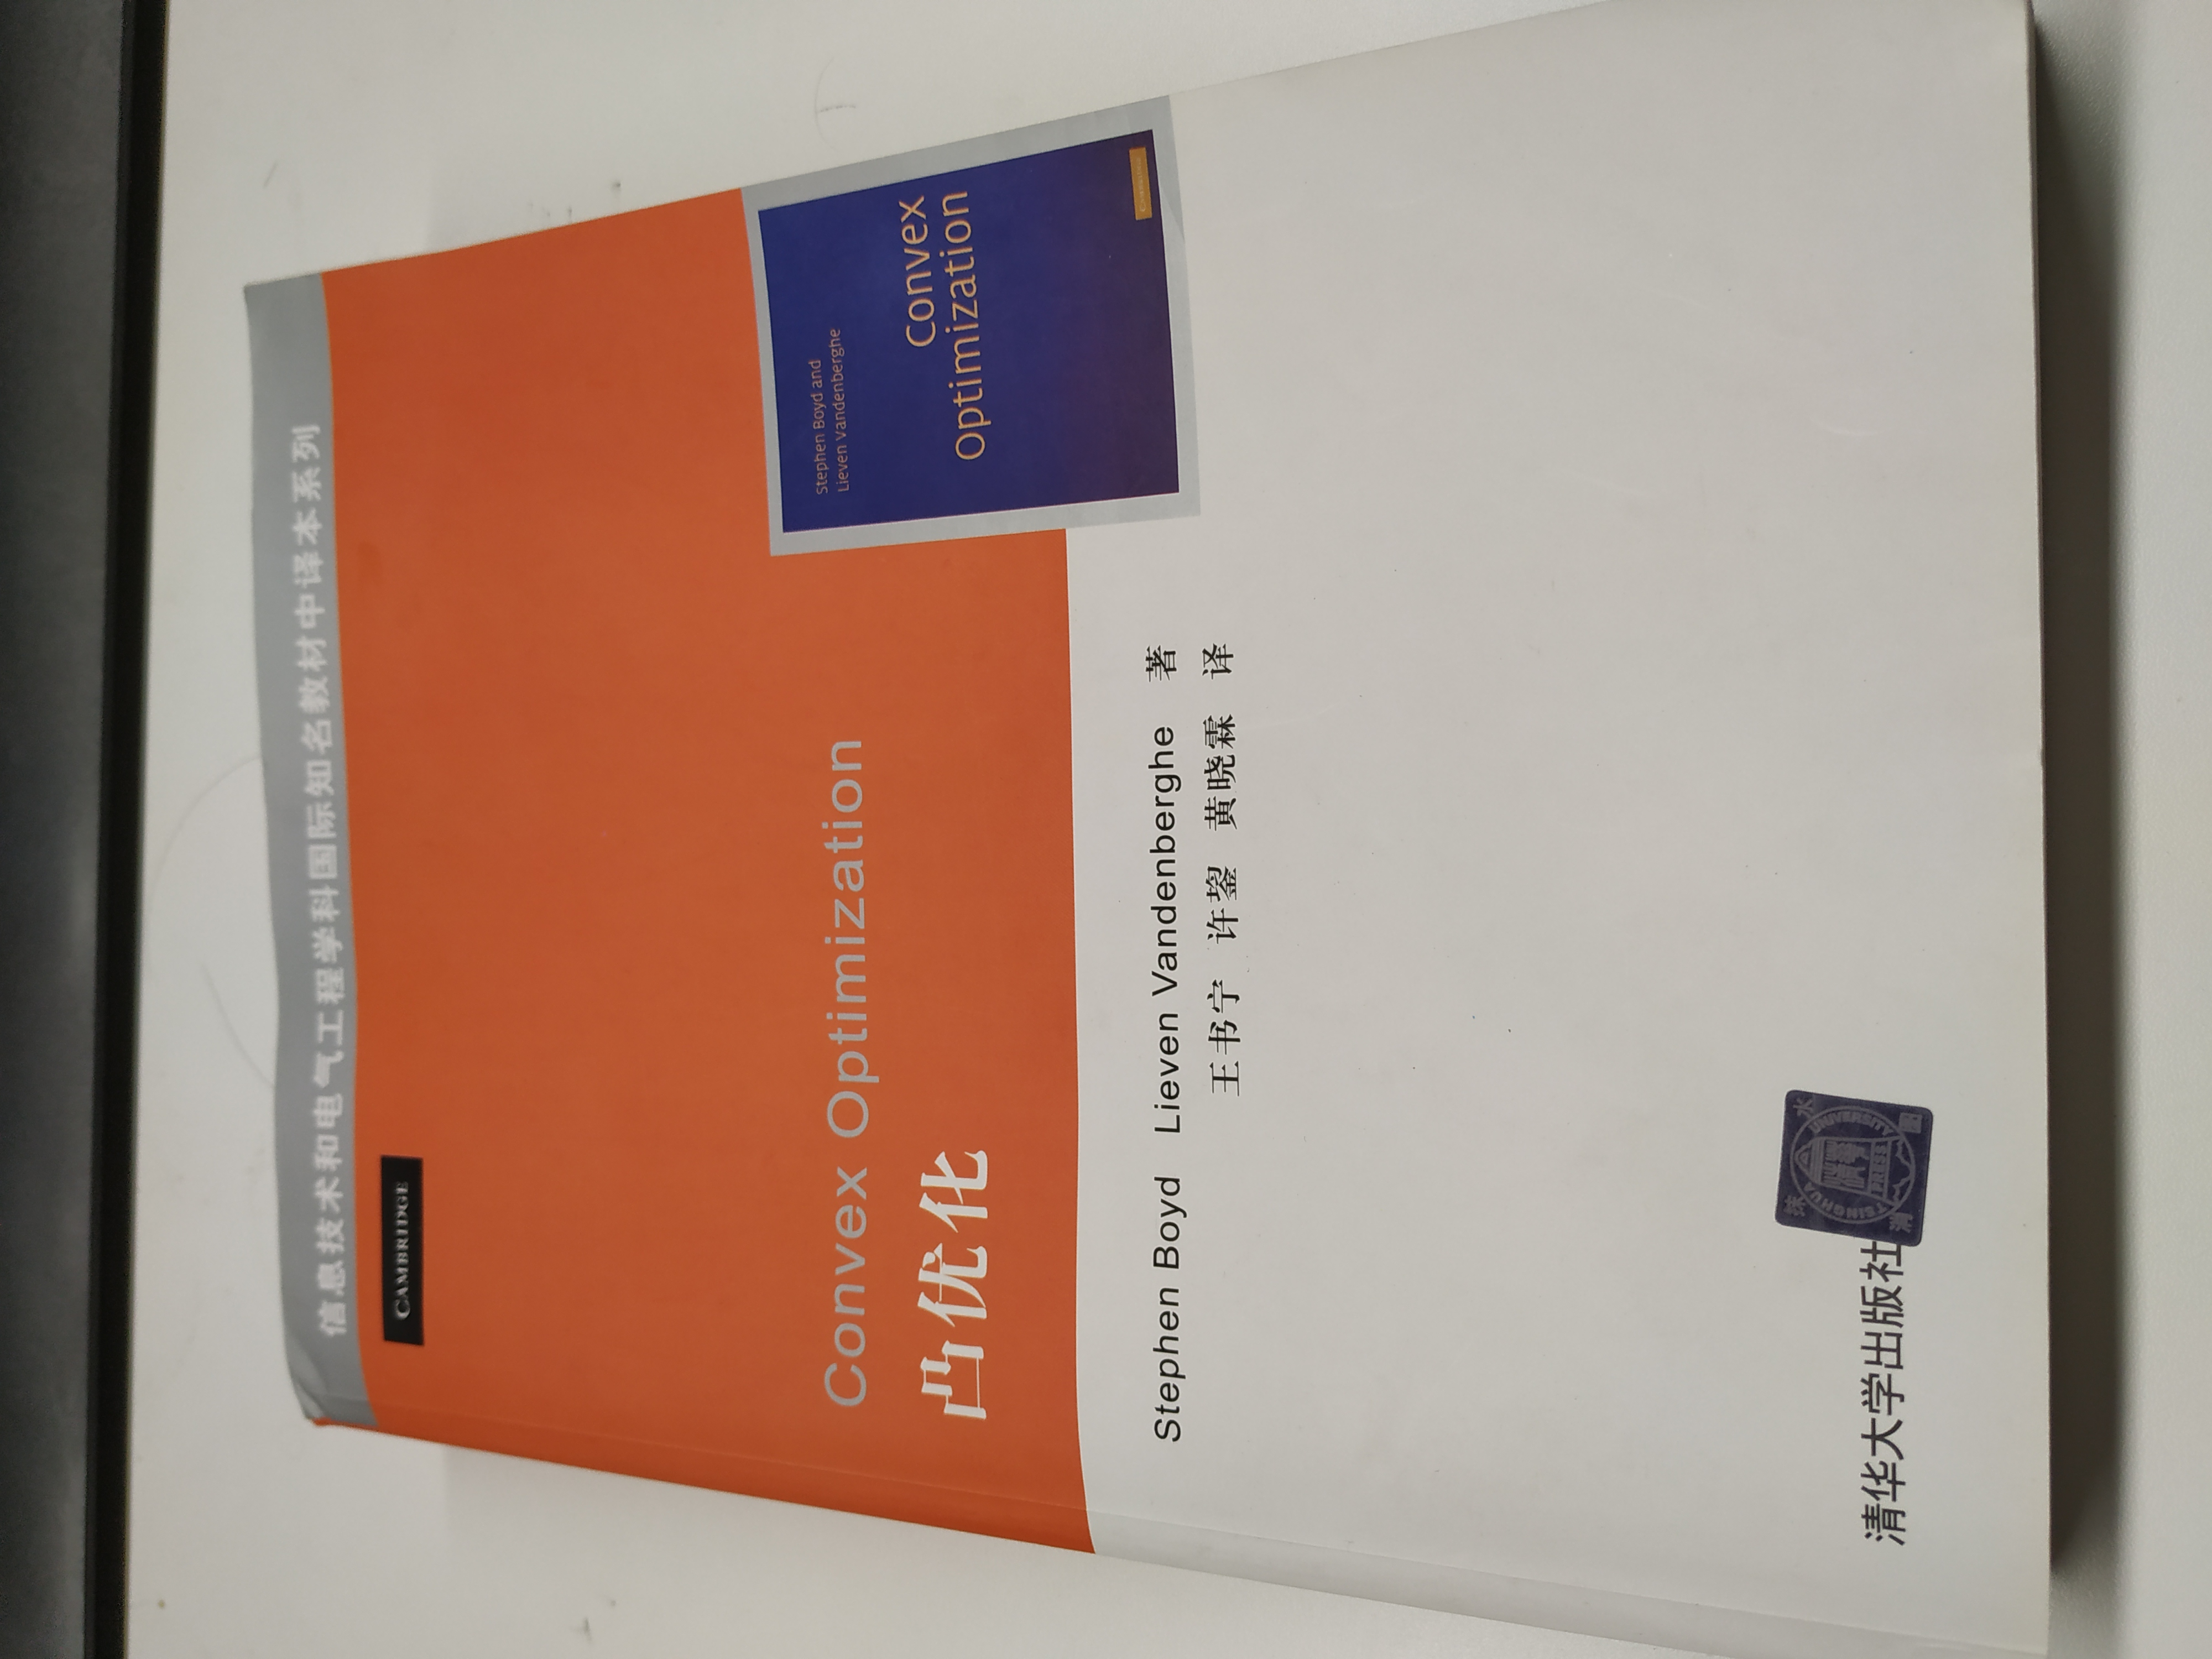
\includegraphics[width=2.5cm,height=3.5cm]{amcl/tyh.jpg}
%     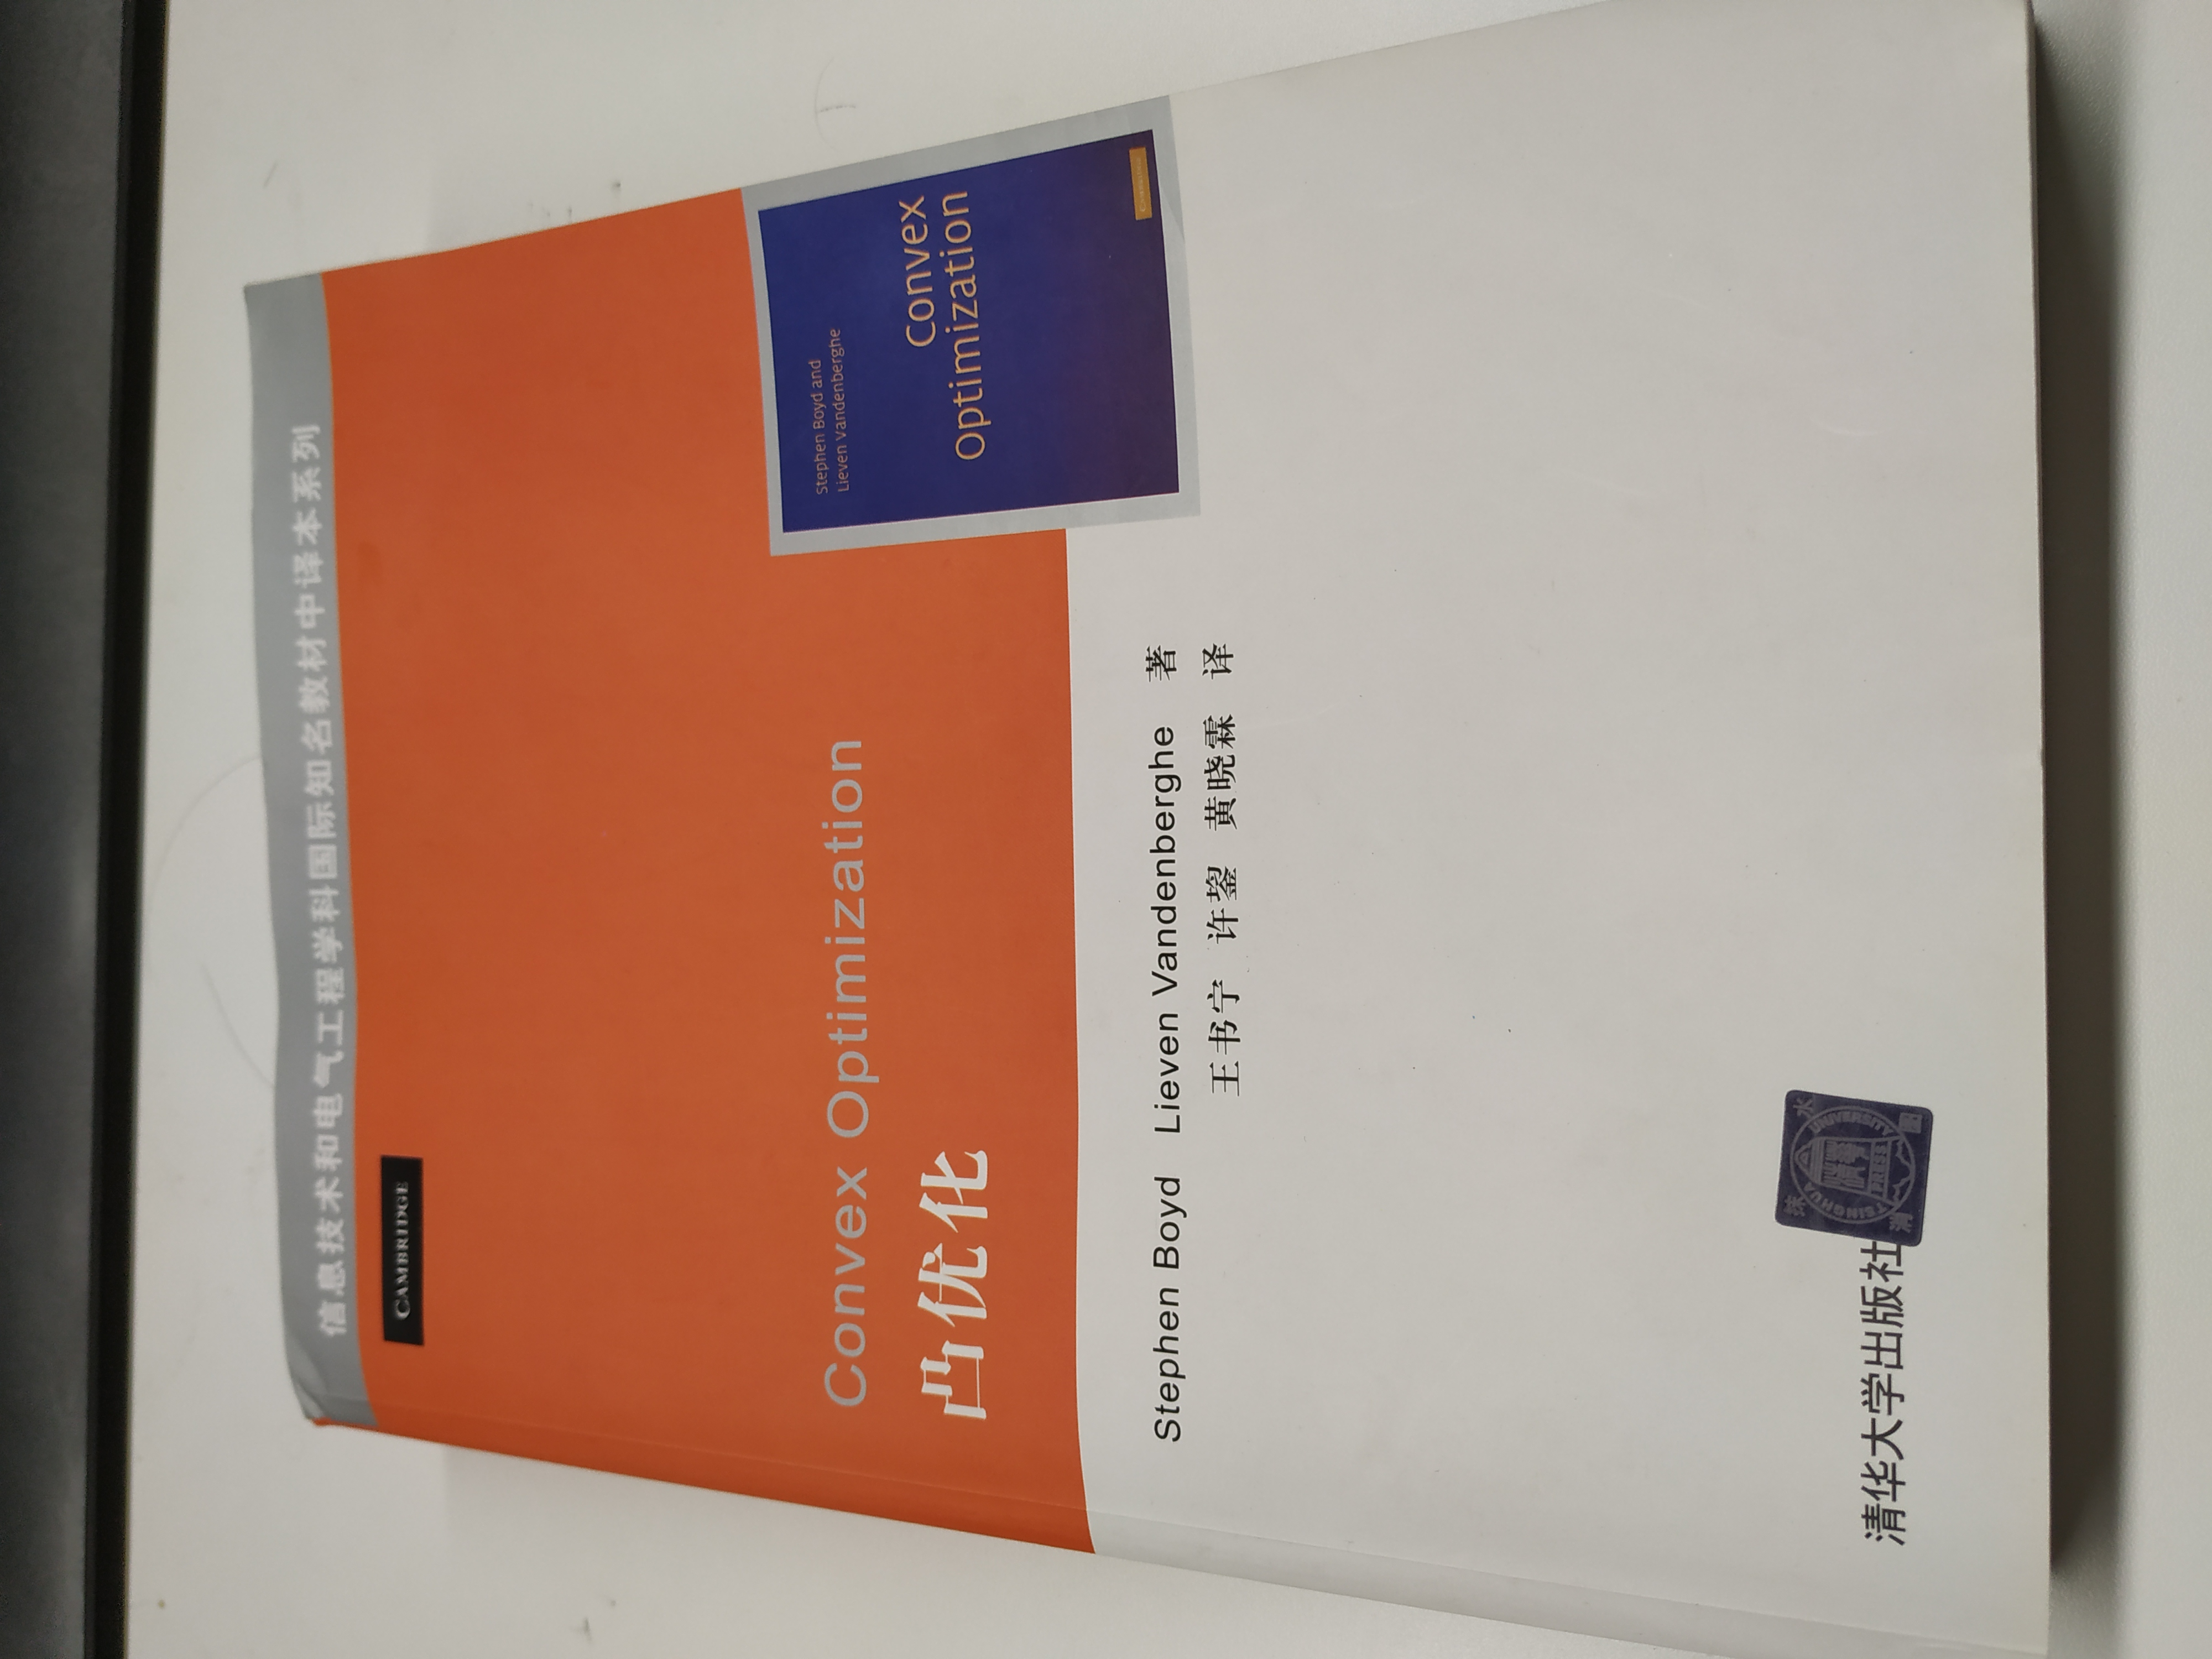
\includegraphics[scale=0.1]{amcl/tyh.jpg}
%     % 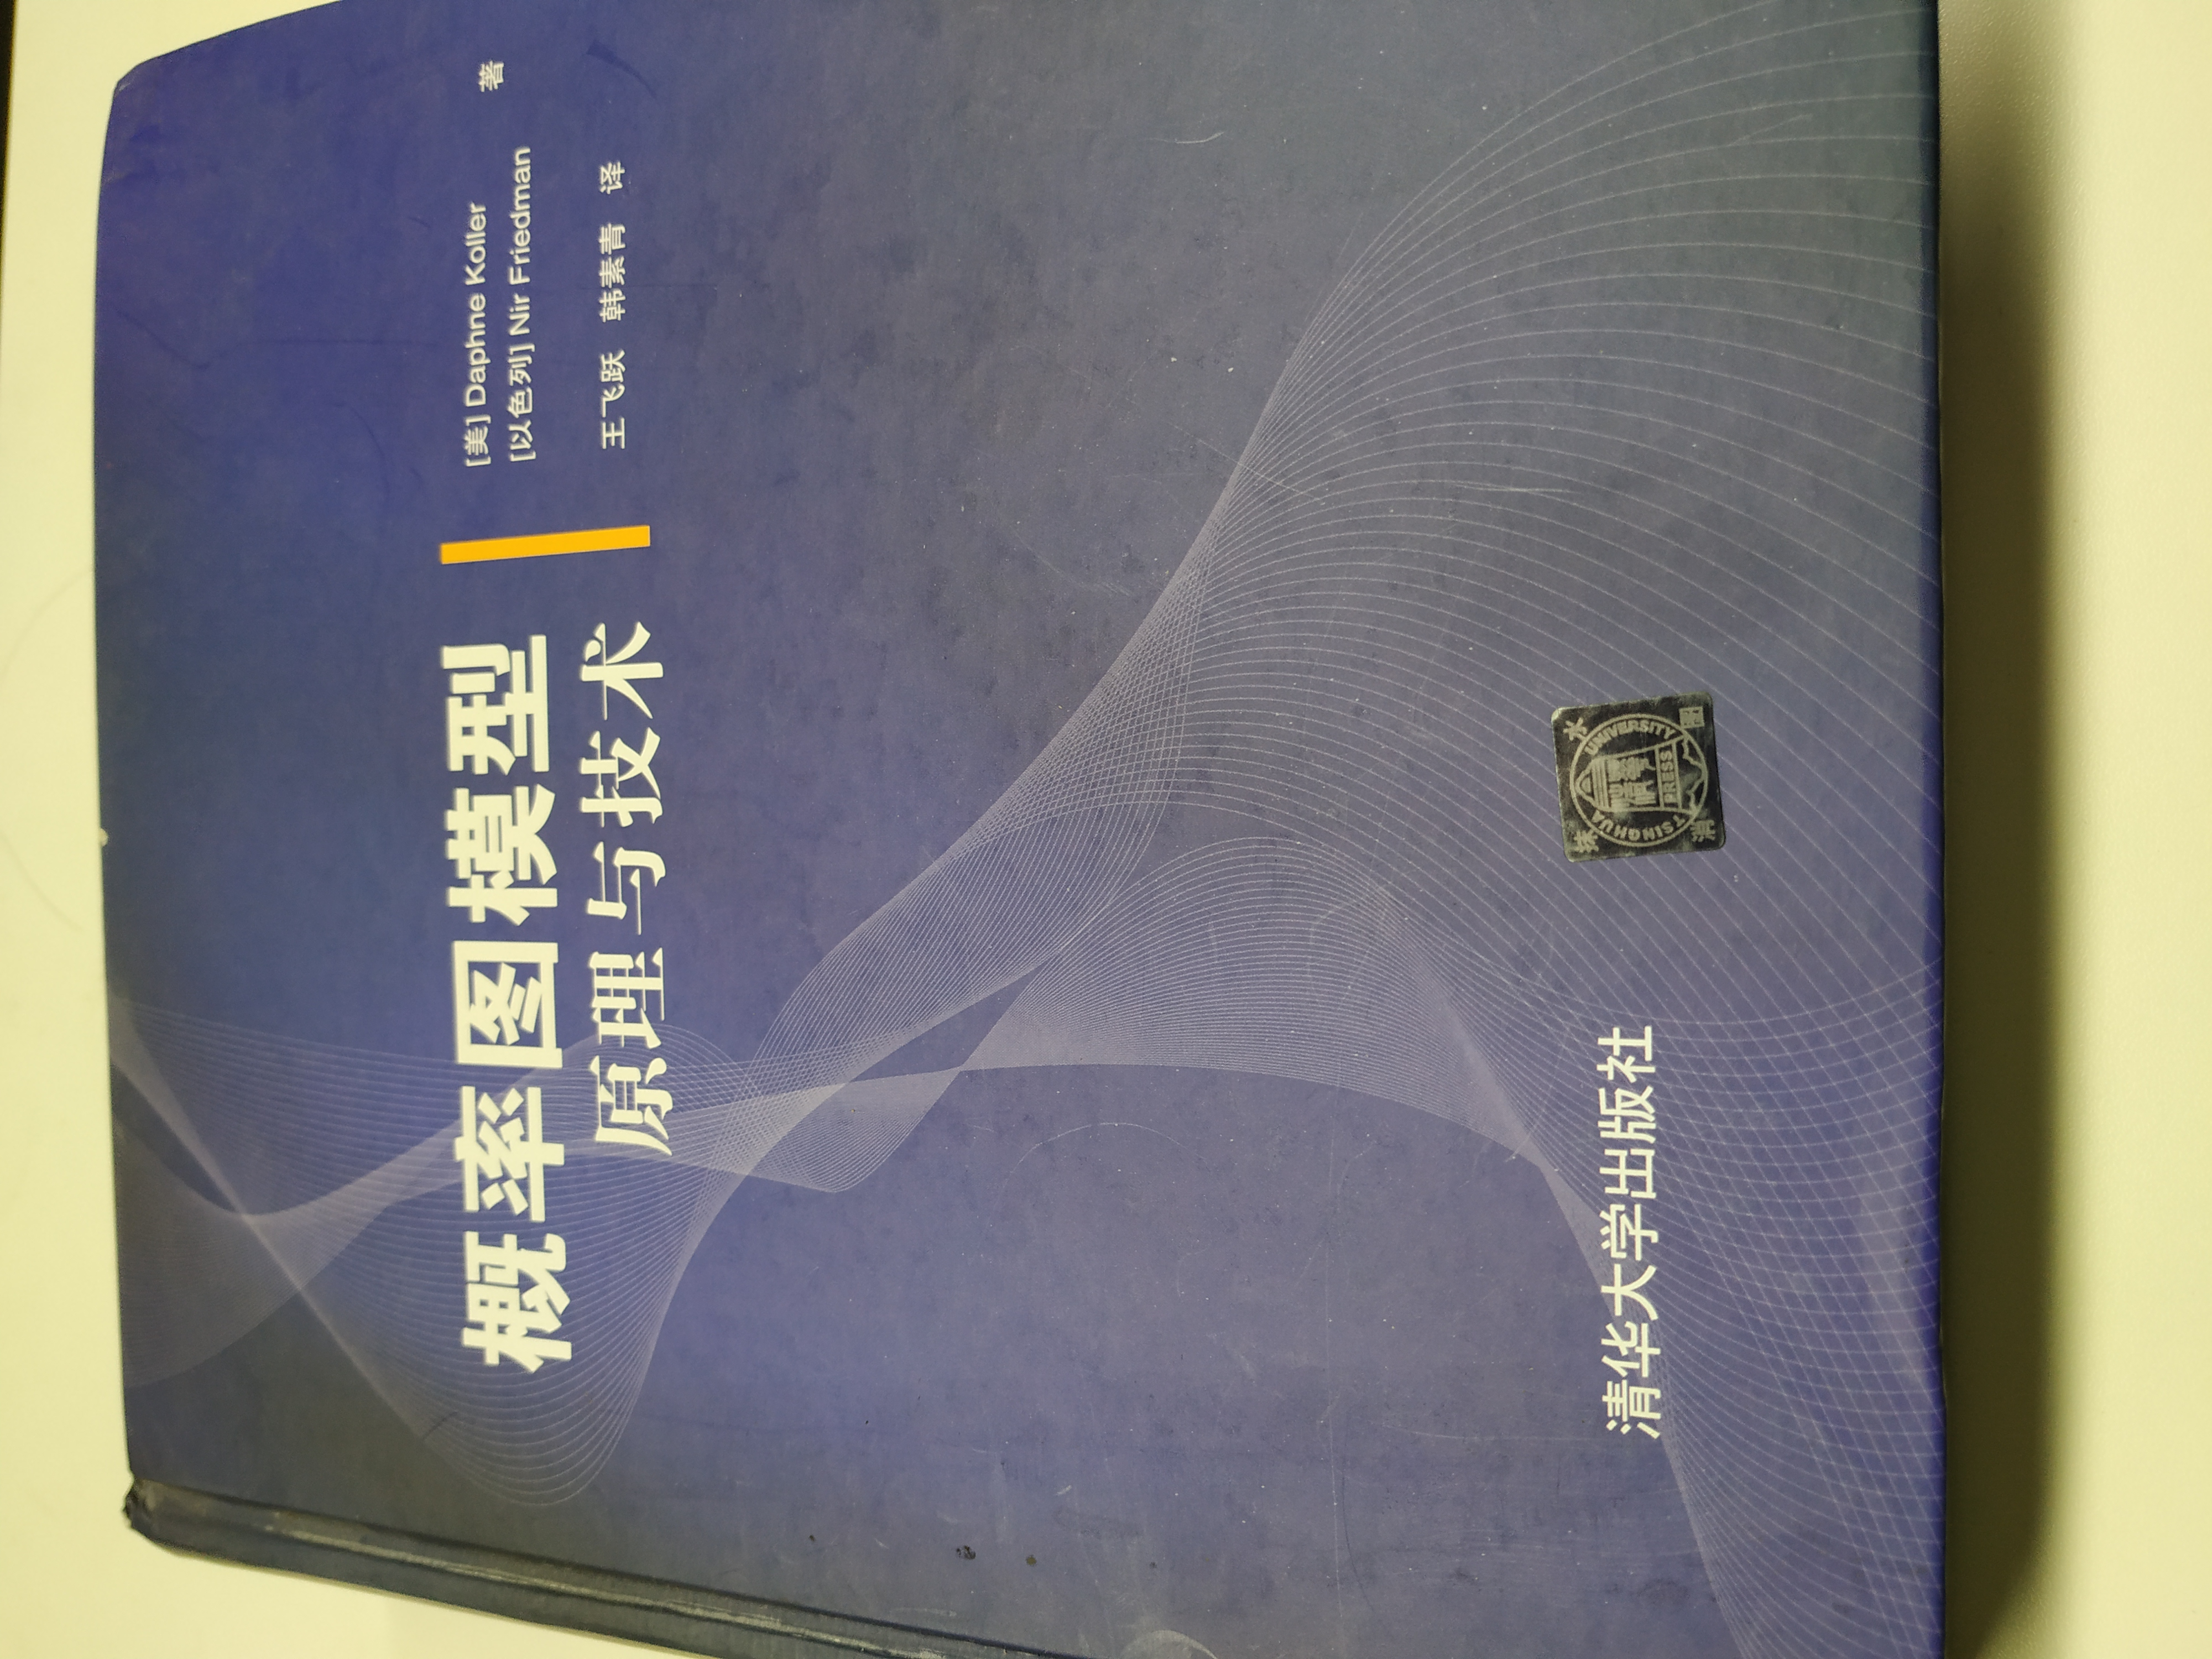
\includegraphics[height=3.0cm]{amcl/gltmx.jpg}
    
%     % 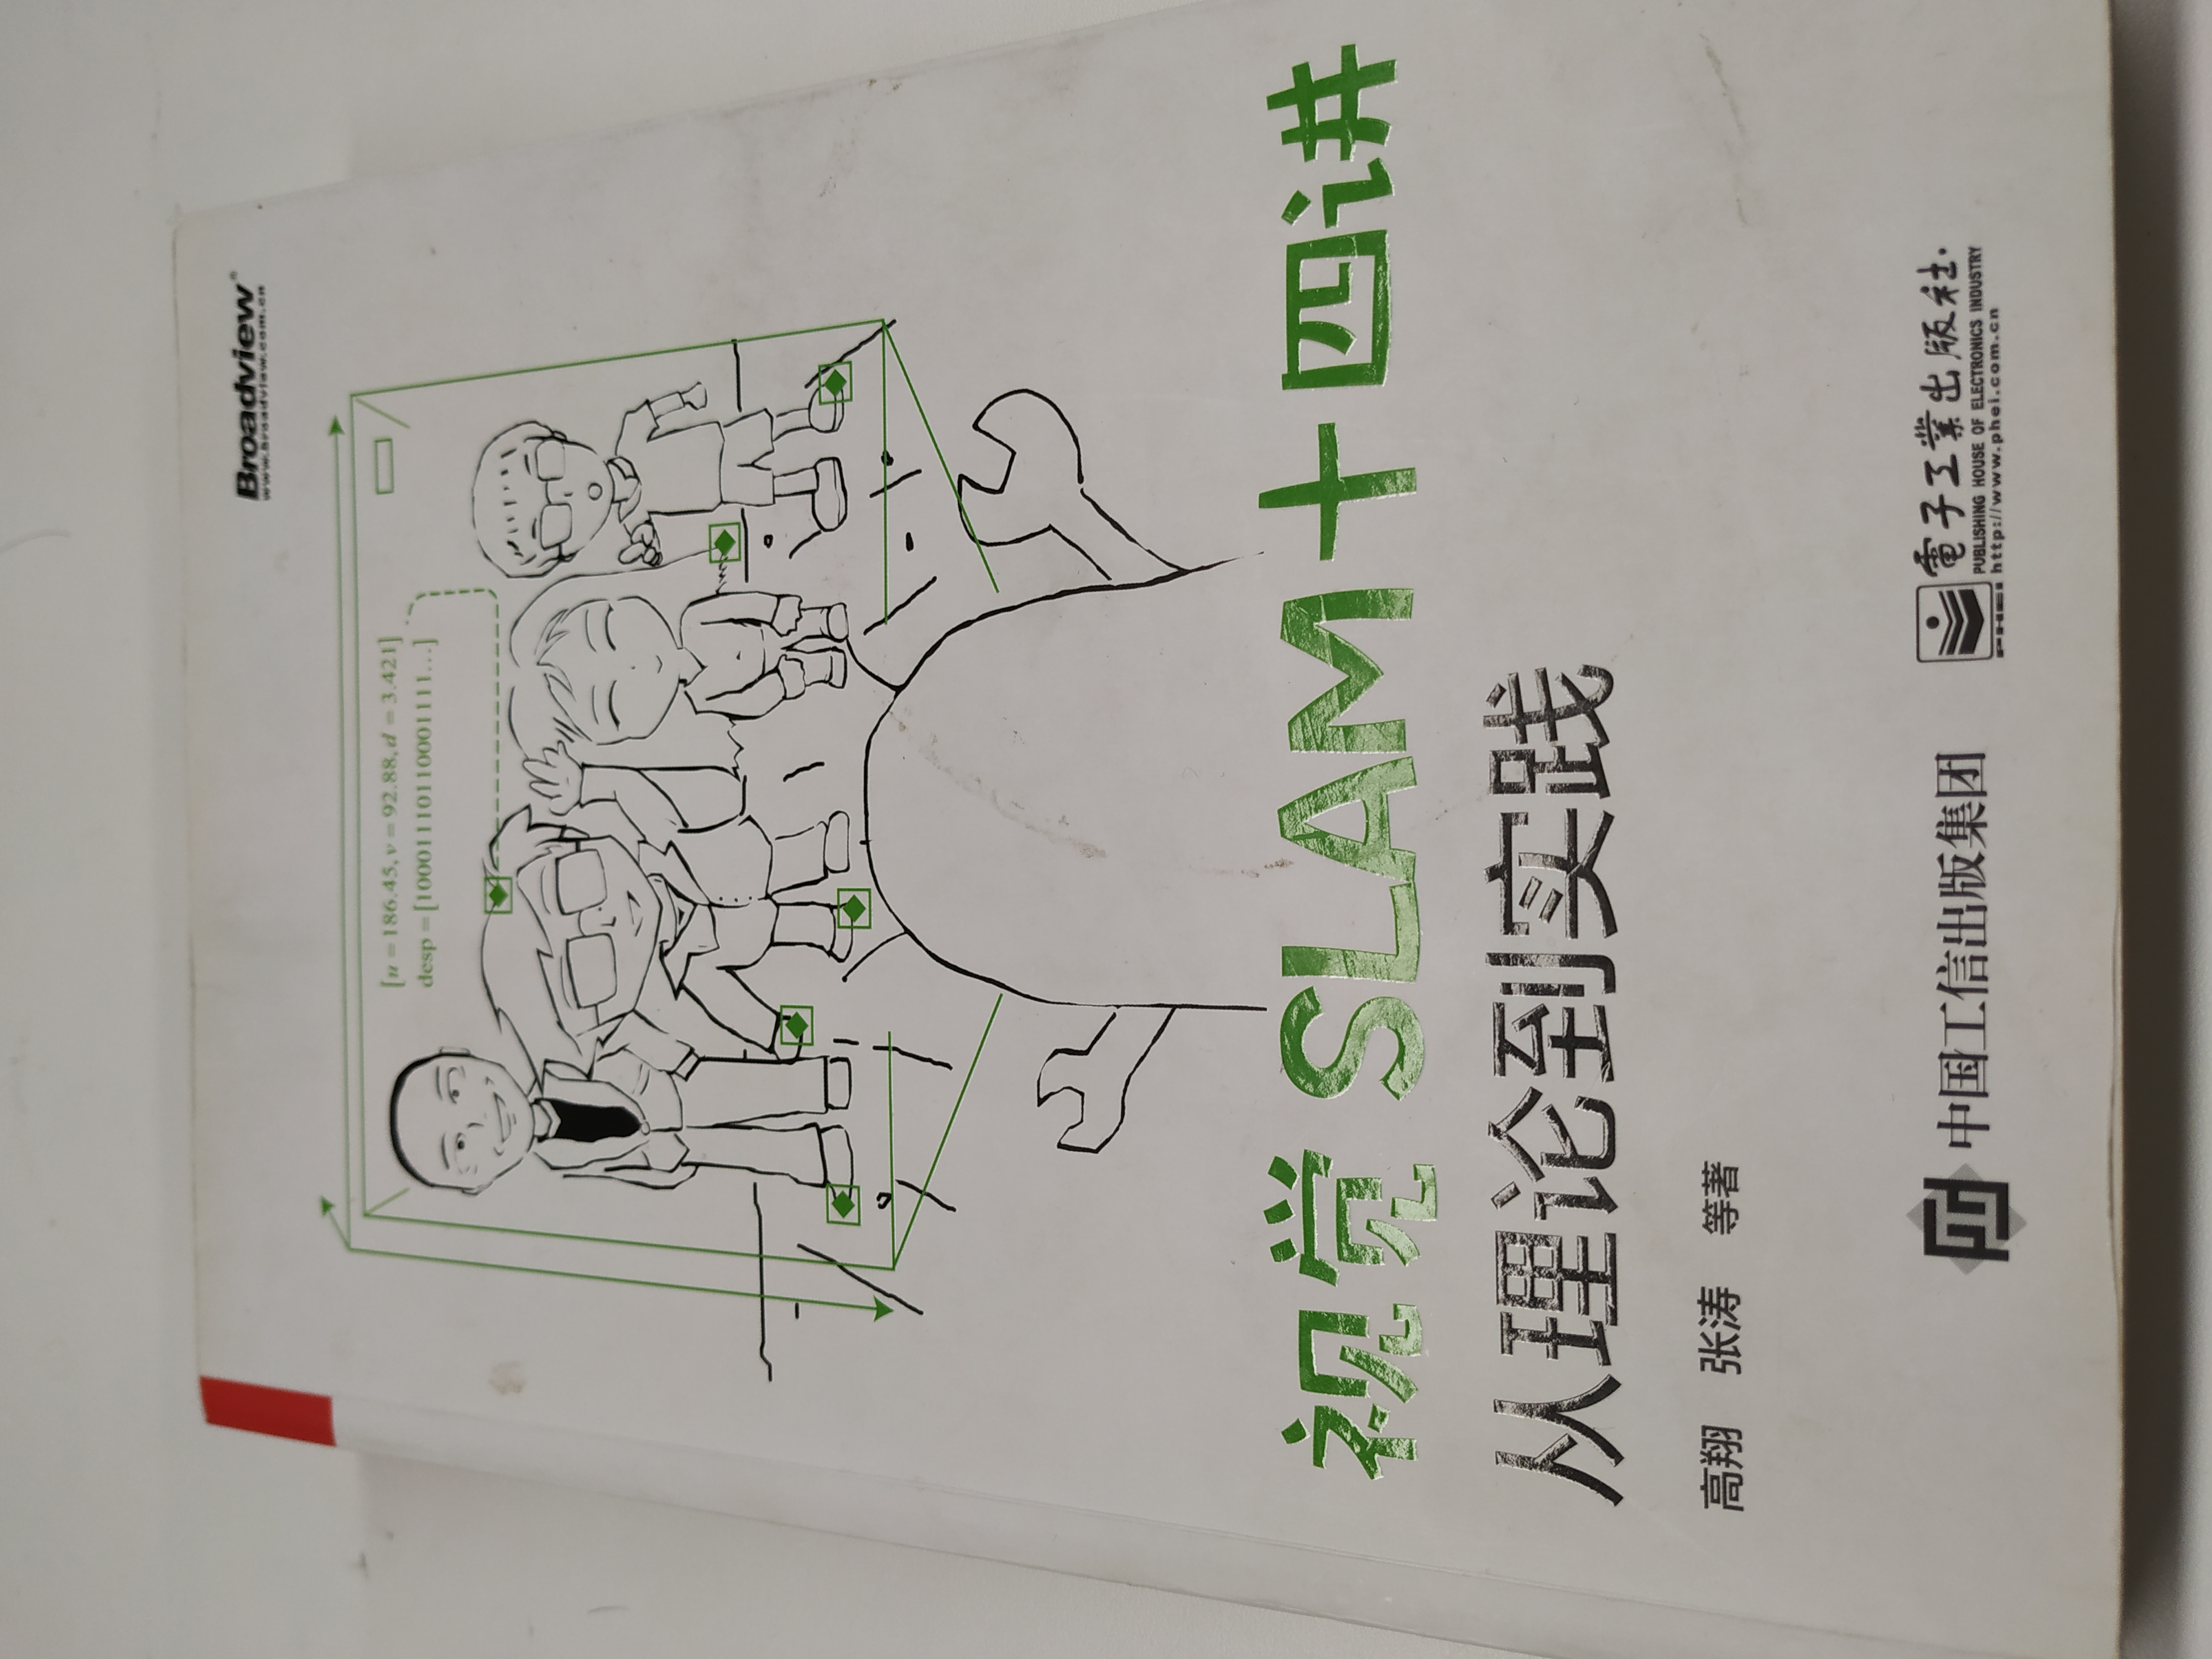
\includegraphics[height=3.0cm]{amcl/sjssj.jpg}
%     % 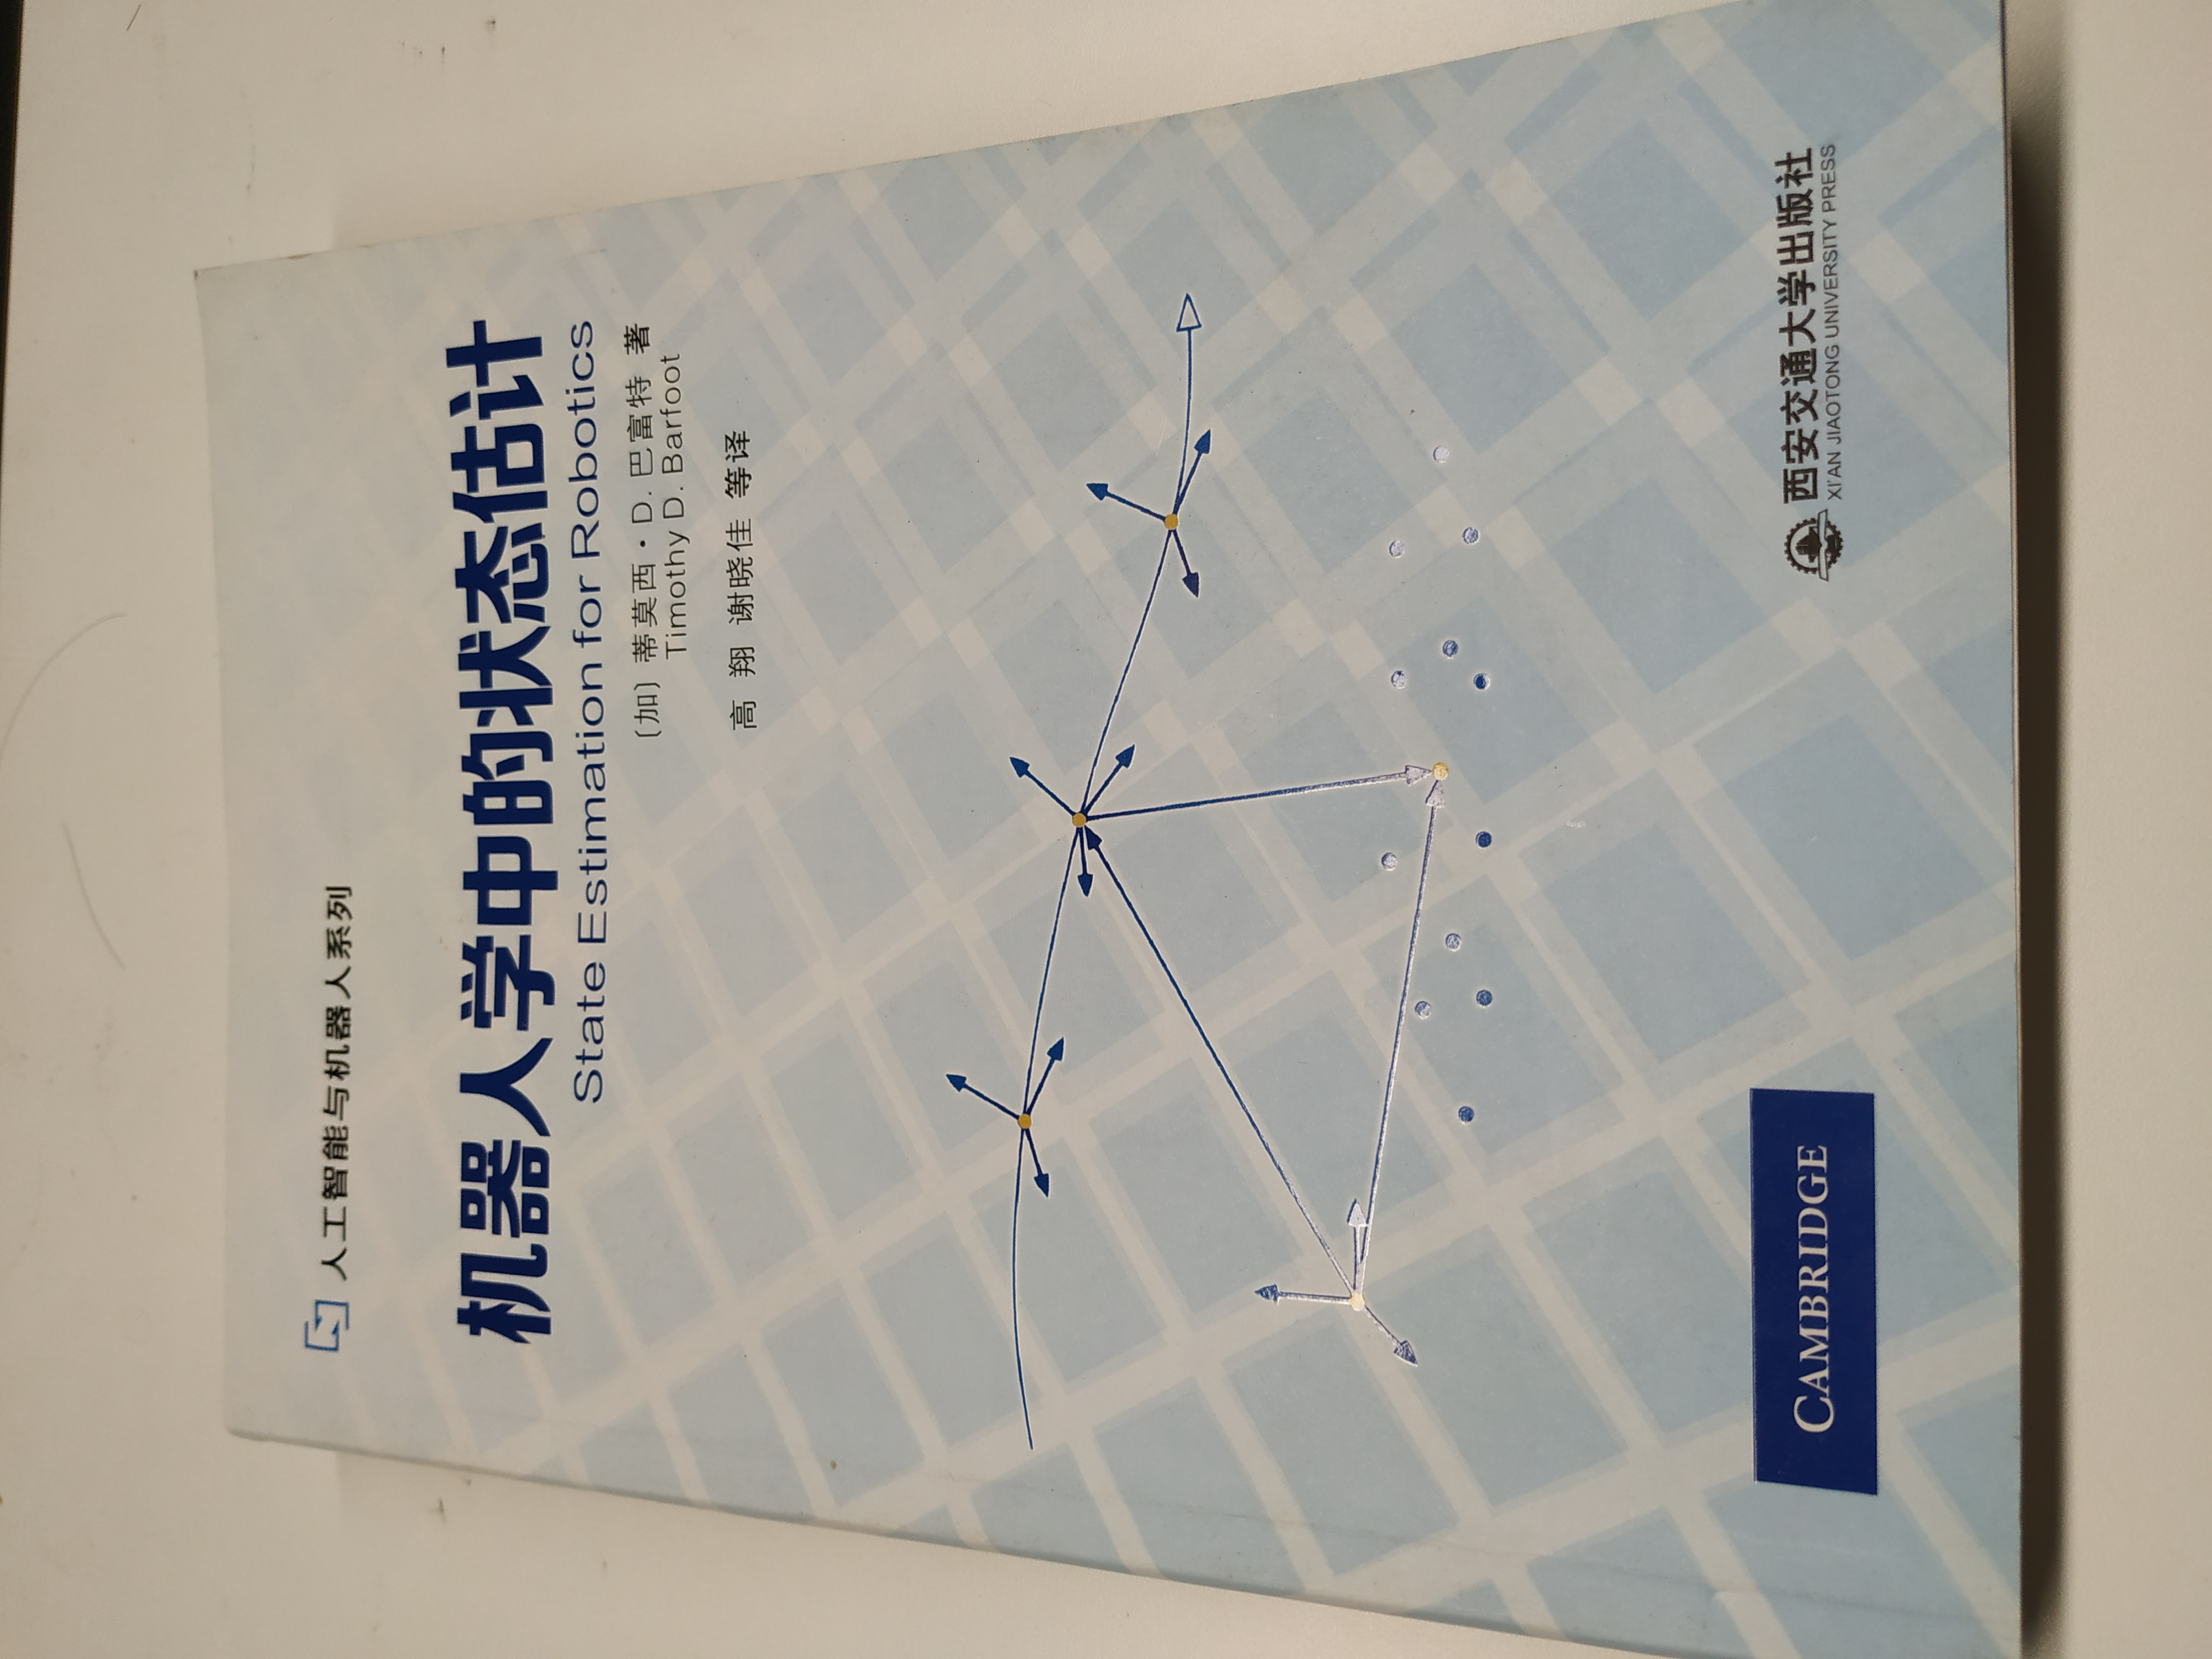
\includegraphics[height=3.0cm]{amcl/jqr.jpg}
%   \end{figure}
% \end{frame}

% \section{c++}

\begin{frame}
\frametitle{explicit关键字}
\begin{enumerate}
	\item 只能修饰一个关键字的构造函数,表明该类构造函数是显示的,而非隐式的,跟它相对应的另一个关键字是implicit, 意思是隐藏的,类构造函数默认情况下即声明为implicit(隐式).
	\item 如果的构造函数只有一个参数时, 那么在编译的时候就会有一个缺省的转换操作:将该{\color{red}构造函数对应数据类型的数据转换为该类对象}.
	\item explicit关键字的作用就是{\color{red}阻止类构造函数的隐式自动转换}.
	\item explicit关键字只对有一个参数的类构造函数有效, 如果类构造函数参数大于或等于两个时, 是不会产生隐式转换的, 所以explicit关键字也就无效了.
	\item 但是, 也有一个例外, 就是当除了第一个参数以外的其他参数都有默认值的时候, explicit关键字依然有效, 此时, 当调用构造函数时只传入一个参数, 等效于只有一个参数的类构造函数
\end{enumerate}

\end{frame}

\begin{frame}
\frametitle{智能指针}
\begin{itemize}
	\item 动态内存管理是通过new/delete 运算符来进行的。由于确保在正确的时间释放内存是很困难的,为了避免内存泄漏,更加容易,安全地使用动态内存,C++11标准库提供了两种智能指针类型来管理动态对象。智能指针的行为类似于常规指针,重要的区别是它负责自动释放所指的对象。
	\begin{enumerate}
		\item std::shared\_ptr ,  允许多个指针指向同一个对象
		\item std::unique\_ptr, 独占所指向的对象
	\end{enumerate}
	\item std::unique\_ptr 是 c++11中用来取代 std::auto\_ptr 指针的指针容器. 它不能与其他unique\_ptr类型的指针对象共享所指对象的内存.这种所有权仅能够通过std::move函数来转移.unique\_ptr是一个删除了拷贝构造函数、保留了移动构造函数的指针封装类型.
	\item 调用release 会切断unique\_ptr 和它原来管理的对象的联系。release 返回的指针通常被用来初始化另一个智能指针或给另一个智能指针赋值.如果不用另一个智能指针来保存release返回的指针,程序就要负责资源的释放
\end{itemize}
\end{frame}

\begin{frame}
\frametitle{algorithm}
\begin{enumerate}
	\item std::min\_element()
	\item std::max\_element()
	\item std::minmax()
	\item std::accumulate()
	\item std::to\_string()
	\item std::atomic()
	\begin{itemize}
		\item std::atomic对int, char, bool等数据结构进行原子性封装,在多线程环境中,对std::atomic对象的访问不会造成竞争-冒险。利用std::atomic可实现数据结构的无锁设计。
		\item std::atomic对象的值的读取和写入可使用load和store实现.
	\end{itemize}
	\item std::this\_thread::yield()
	\begin{itemize}
		\item 当前线程放弃执行,操作系统调度另一线程继续执行。即当前线程将未使用完的“CPU时间片”让给其他线程使用,等其他线程使用完后再与其他线程一起竞争"CPU"。
	\end{itemize}
	\item std::this\_thread::sleep\_for()
	\begin{itemize}
		\item 表示当前线程休眠一段时间,休眠期间不与其他线程竞争CPU,根据线程需求,等待若干时间。
	\end{itemize}
\end{enumerate}
\end{frame}

\begin{frame}
\frametitle{C++11内存模型}
C++11引入了多线程,同时也引入了一套内存模型。从而提供了比较完善的一套多线程体系。在单线程时代,一切都很简单。没有共享数据,没有乱序执行,所有的指令的执行都是按照预定的时间线。但是也正是因为这个强的同步关系,给CPU提供的优化程度也就相对低了很多。无法体现当今多核CPU的性能。因此需要弱化这个强的同步关系,来增加CPU的性能优化。\href{https://www.cnblogs.com/navono007/p/5746048.html}{(参考)}

C++11提供了6种内存模型:
\begin{enumerate}
	\item memory\_order\_relaxed
	\item memory\_order\_consume
	\item memory\_order\_acquire
	\item memory\_order\_release
	\item memory\_order\_acq\_rel
	\item memory\_order\_seq\_cst
\end{enumerate}
\end{frame}

\begin{frame}
\frametitle{C++11内存模型}
原子类型的操作可以指定上述6种模型的中的一种,用来控制同步以及对执行序列的约束。从而也引起两个重要的问题:
\begin{enumerate}
	\item 哪些原子类型操作需要使用内存模型?
	\item 内存模型定义了哪些同步语义(synchronization )和执行序列约束(ordering constraints)?
\end{enumerate}

原子操作可分为3大类:
\begin{enumerate}
	\item 读操作:memory\_order\_acquire, memory\_order\_consume
	\item 写操作:memory\_order\_release )
	\item 读-修改-写操作:memory\_order\_acq\_rel, memory\_order\_seq\_cst
	\item 未被列入分类的memory\_order\_relaxed没有定义任何同步语义和顺序一致性约束
\end{enumerate}

\end{frame}

\begin{frame}
\frametitle{C++11内存模型}
 C++11中有3种不同类型的同步语义和执行序列约束:
\begin{enumerate}
	\item 顺序一致性(Sequential consistency):对应的内存模型是memory\_order\_seq\_cst
	\item 请求-释放(Acquire-release):对应的内存模型是memory\_order\_consume,memory\_order\_acquire,memory\_order\_release,memory\_order\_acq\_rel
	\item 松散型(非严格约束。Relaxed):对应的内存模型是memory\_order\_relaxed
\end{enumerate}

下面对上述3种约束做一个大概解释:
\begin{enumerate}
	\item Sequential consistency:指明的是在线程间,建立一个全局的执行序列
	\item Acquire-release:在线程间的同一个原子变量的读和写操作上建立一个执行序列
	\item Relaxed:只保证在同一个线程内,同一个原子变量的操作的执行序列不会被重排序(reorder),这种保证也称之为modification order consistency,但是其他线程看到的这些操作的执行序列式不同的。
	\item 还有一种consume模式,也就是std::memory\_order\_consume。这个模式主要是引入了原子变量的数据依赖。
\end{enumerate}

\end{frame}

\begin{frame}
\frametitle{GUARDED\_BY 和EXCLUDES属性字}


这些都是在Clang Thread Safety Analysis(线程安全分析)中定义的属性,Clang Thread Safety Analysis是C ++语言扩展,它警告代码中潜在的竞争条件。分析是完全静态的(即编译时);没有运行时开销。该分析仍在积极开发中,但已经足够成熟,可以在工业环境中进行部署。它是由Google与CERT / SEI合作开发的,并广泛用于Google的内部代码库中。
\begin{itemize}
	\item GUARDED\_BY是{\color{red}数据成员}的属性,该属性声明数据成员受给定功能保护。{\color{red}对数据的读操作需要共享访问,而写操作则需要互斥访问}。
该GUARDED\_BY属性声明线程必须先锁定listener\_list\_mutex才能对其进行读写listener\_list,从而确保增量和减量操作是原子的.
	\item EXCLUDES是{\color{red}函数或方法}的属性,该属性声明调用方不拥有给定的功能。该注释{\color{red}用于防止死锁}。许多互斥量实现都不是可重入的,因此,如果函数第二次获取互斥量,则可能发生死锁。
在上面代码中的EXCLUDES表示的意思是:调用listener\_disconnect()函数的调用用不能拥有listener\_list\_mutex锁。

\end{itemize}
\end{frame}

\begin{frame}
\frametitle{content}
\begin{itemize}
	\item mutable 关键字: mutable 是为了突破 const 的限制而设置的。可以用来修饰一个类的成员变量。被 mutable 修饰的变量,将永远处于可变的状态,即使是 const 函数中也可以改变这个变量的值。
\end{itemize}
\end{frame}







% \section{ceres}

\begin{frame}
\frametitle{ceres库 \hfill 
\includegraphics[trim=0 0 0 0 0.1,height=0.5cm,clip]{logo.png}}

Ceres库主要用于求解无约束或者有约束的最小二乘问题.其数学形式如下:

\begin{equation}
	\frac{1}{2} \sum_i 
\end{equation}


http://gaoyichao.com/Xiaotu/?book=Cartographer%E6%BA%90%E7%A0%81%E8%A7%A3%E8%AF%BB&title=%E5%9F%BA%E4%BA%8ECeres%E5%BA%93%E7%9A%84%E6%89%AB%E6%8F%8F%E5%8C%B9%E9%85%8D%E5%99%A8
\end{frame}


\begin{comment}

\end{comment}
\begin{frame}
\frametitle{ceres \hfill 
\includegraphics[height=0.5cm]{logo.png}}


\end{frame}

\begin{comment}
\end{comment}
\begin{frame}[fragile]
\frametitle{Ceres \hfill 
\includegraphics[height=0.5cm]{logo.png}}
\begin{columns}
	\column{0.5\textwidth}
	\begin{itemize}
		\item Ceres库主要用于求解无约束或者有约束的最小二乘问题.其数学形式如下:

		
		\begin{equation}\label{eq:ceres}
		\begin{split}
		& \mathop{\min}_{x} \frac{1}{2} \sum_i \rho_i(\| f_i(x_1, ..., x_k) \|^2) \\
		& s.t. \ \ \ l_j \leq x_j \leq u_j \\
		\end{split}
		\end{equation}
		\vspace{0.2cm}
		\item 在Ceres库中,优化参数$x_1, ..., x_k$被称为{\color{red}参数块(ParameterBlock)},他们的取值就是我们要寻找的解.
		$l_j, u_j$分别是第$j$个优化参数$x_j$的下界和上界.
		表达式$\rho_i(\| f_i(x_1, ..., x_k) \|^2)$被称为{\color{red}残差项(ResidualBlock)}.
		其中,$f(\cdot)$是{\color{red}代价函数(CostFunction)},$\rho_i(\cdot)$是关于代价函数平方的{\color{red}核函数(LossFunction)}.
		核函数存在的意义主要是为了降低野点(outliners)对解的影响.
	\end{itemize}
	\column{0.5\textwidth}
	\begin{itemize}
		\item 很多时候最小二乘是拿来做曲线拟合的,实际上只要能够把问题描述成式\ref{eq:ceres}的形式,就可以使用Ceres来求解.
		使用方法如下边示例代码所示.
		%一般需要定义三个对象,problem用于描述将要求解的问题,options提供了很多配置项,summary用于记录求解过程.
\vspace{0.3cm}
\begin{lstlisting}[frame=shadowbox]  
ceres::Problem problem;
ceres::Solver::Options options;
ceres::Solver::Summary summary;
\end{lstlisting}

		\item 然后,可以想下边那样通过problem对象的接口AddResidualBlock描述各个残差项的计算方式.
		这个接口有三个参数,都是通过指针的形式提供对象.
		%针对每个残差项,都需要提供一个代价函数以及核函数对象,
		%而params则是所有残差项共有的,就是我们希望优化的参数.
\begin{lstlisting}[frame=shadowbox]		
problem.AddResidualBlock(cost_function_1, loss_function_1, params);
......
problem.AddResidualBlock(cost_function_n, loss_function_n, params);
\end{lstlisting}

	\end{itemize}

\end{columns}
\end{frame}

\begin{comment}
\end{comment}
\begin{frame}[fragile]
\frametitle{Ceres \hfill 
\includegraphics[height=0.5cm]{logo.png}}
\begin{columns}
	\column{0.5\textwidth}
	\begin{itemize}
		\item 关于cost\_function,除了要提供代价函数的计算方法外,还要明确其求导方法.
		求导方法完全可以以仿函数的形式自己定义一个,但更多时候都在使用Ceres提供的AutoDifferentCostFunction进行求导.
		所以,经常可以看到类似下面示例的调用方法.
		%类AutoDiffCostFunction是一个模板类,其模板参数类表中的CostFunction是计算残差项代价的仿函数类型,
		%m是CostFunction所提供的残差项数量,n则是优化参数的数量.
		%仿函数技巧的一个优点,它能利用对象的成员变量来存储更多的函数内部参数.
\begin{columns}	
	\column{0.8\textwidth}
	\begin{minipage}{6.5cm}
        \begin{lstlisting}[frame=shadowbox]  
problem.AddResidualBlock(new ceres::AutoDiffCostFunction<CostFunction, m, n>(
    new CostFunction(/*构造参数*/)), loss_function, params);
        \end{lstlisting}
	\end{minipage}
\end{columns}

		\item 代价函数本身的计算,要求以仿函数的形式提供一个重载运算符"()"的类,并在该重载中完成代价的计算,如右边示例:
		\vspace{0.2cm}
	\end{itemize}
	\column{0.5\textwidth}

\begin{columns}	
\column{0.7\textwidth}
\begin{minipage}{5cm}
\begin{lstlisting}[frame=shadowbox]  
class CostFunction {
public: 
    template <typename T>
    bool operation()(cost T* const params, T* cost) const {
        // 必要的运算之后,更新各个cost
        cost[0] = value_0;
        ......
        cost[m] = value_m;
        return true;
    }
}
\end{lstlisting}
\end{minipage}
\end{columns}
\end{columns}
\end{frame}

%%%%%%%%%%%%%%%%templete%%%%%%%%%%%%%%%%%%%%%
\begin{comment}
\end{comment}
\begin{frame}[fragile]
\frametitle{分支定界方法 \hfill 
\includegraphics[height=0.5cm]{logo.png}}
\begin{columns}
	\column{0.5\textwidth}
	\begin{itemize}
		\item 
		\vspace{0.2cm}
	\end{itemize}
	\column{0.5\textwidth}
	\begin{itemize}
		\item 
\begin{columns}	
	\column{0.8\textwidth}
	\begin{minipage}{6.5cm}
		\begin{lstlisting}[frame=shadowbox]  
		\end{lstlisting}
	\end{minipage}
\end{columns}
	\end{itemize}
\end{columns}
\end{frame}

%%%%%%%%%%%%%%%%templete%%%%%%%%%%%%%%%%%%%%%


% \section{分支定界闭环检测的原理和实现}


\begin{comment}
1.$\epsilon = [\epsilon_x, \epsilon_y, \epsilon_\theta]^T$表示机器人在地图坐标系下的位姿.
$T_\epsilon$表示位姿估计的坐标变换.


\end{comment}
\begin{frame}
\frametitle{算法原理 \hfill 
\includegraphics[height=0.5cm]{logo.png}}

在Local SLAM中,通过Submap中的Scan-to-Map匹配得到了一个比较理想的机器人位姿估计.
但是由于Local SLAM只使用了一段时间内的局部信息,所以定位误差会随时间积累.
为了能够进一步降低局部累积误差的影响,Cartographer通过Pixel-accurate扫描匹配来进行回环检测,进一步优化机器人的位姿估计.

~\\

%\hspace*{\fill}

计$H=\{h_1, ..., h_k, ..., h_K\}$为传感器扫描到K个hit点集合,$h_k$是第k个hit点在机器人坐标系下的位置坐标.那么$h_k$在地图坐标系下的坐标可以表示为:

\begin{equation}
	T_\epsilon h_k = 
	\begin{bmatrix}
	\cos{\epsilon_\theta } & -\sin\epsilon_\theta \\
	\sin\epsilon_\theta & \cos\epsilon_\theta 
	\end{bmatrix}
	h_k +
	\begin{bmatrix}
	\epsilon_x \\ \epsilon_y
	\end{bmatrix}
\end{equation}

Pixel-accurate扫描匹配问题可以用下式描述:

\begin{equation}
	\epsilon ^* = \mathop{argmax}\limits_{\epsilon \in W} \sum_{k=1}^K M_{nearest}(T_\epsilon h_k)
\end{equation}

式中,$W$是一个搜索窗口,$M_{nearest}(T_\epsilon h_k)$是离$T_\epsilon h_k$最近的栅格单元的占用概率.
可以解释为,在搜索窗口$W$中找到一个最优的位姿,使得hit点集合出现的概率最大化.

%~\\



\end{frame}


\begin{frame}[fragile]
\frametitle{暴力搜索方法}

\begin{columns}
	\column{0.4\textwidth}	
		有一种暴力搜索的方法,如右图所示,这是一种枚举的方法.
		给定搜索步长$r$和$\delta_\theta$,搜索过程以$\epsilon_0$为中心,通过三层循环遍历所有的Pixel并选出得分最高的位姿作为输出$\epsilon^*$
	\column{0.5\textwidth}
暴力匹配的algorithm如下:
\begin{algorithmic}[1]
\State \textbf{Algorithm 1} Naive algorithm for (BBS)
\State $best\_score \leftarrow - \infty$
\State $\text{for } j_x = -w_x \text{ to } w_x \text{ do}$
\State \quad $\text{for } j_y = -w_y \text{ to } w_y \text{ do}$
\State \qquad $\text{for } j_\theta = -w_\theta \text{ to } w_\theta \text{ do}$
\State \qquad \quad $score \leftarrow \sum_{k=1}^K M_{nearset} (T_{\xi 0}+(rj_x,rj_y,\delta_\theta rj_\theta)h_k)$
\State \qquad \quad $\text{if } score > best\_score \text{ then}$
\State \qquad \qquad $match \leftarrow \xi 0 + (rj_x,rj_y,\delta_\theta rj_\theta)$
\State \qquad \qquad $best\_score \leftarrow score$
\State \qquad \quad end if
\State \qquad end for
\State \quad end for
\State end for
\State return $best\_score \text{ and } match \text{ when set.}$
\end{algorithmic}
\end{columns}

\end{frame}

\begin{comment}

\end{comment}
\begin{frame}
\frametitle{分支定界方法 \hfill 
\includegraphics[height=0.45cm]{logo.png}}
\begin{columns}
	\column{0.4\textwidth}
		
	\begin{itemize}
		\item 暴力搜索方法中如果搜索窗口过大或者搜索步长太小,都将导致整个搜索过程耗时过长.
		\item Cartographer使用分支定界方法搜索,该算法的基本思想是:
		\begin{itemize}
			\item 用一颗树表示整个解空间.%,其根节点代表整个搜索窗口$W$.
			\item 每一个节点的孩子都是对该节点所代表的搜索空间的一个划分.
			\item 每个叶节点都对应着一个解.
		\end{itemize}
	\end{itemize}
	
	\column{0.4\textwidth}
	整个搜索过程的基本思想:
	\begin{itemize}
		\item 不断地分割搜索空间,这个过程称为{\color{red}分支}.
		\item 为每次分支之后的孩子节点确定一个上界,这个过程称为{\color{red}定界}.
		\item 如果一个节点的定界超出了已知最优解的值,这意味着该节点下的所有解都不可能比已知解更优,将不在分支该节点.
		%缩小搜索范围,提高算法效率
	\end{itemize}
\end{columns}

\end{frame}

\begin{frame}[fragile]
\frametitle{branch and bound}
分支定界algorithm如下:
\begin{columns}
	\column{0.5\textwidth}
	\begin{algorithmic}[1]
		\State \textbf{Algorithm 2} DFS branch and bound scan matcher for (BBS)
		\State $best\_score \leftarrow score\_threshold$
		\State Compute and memorize a score for each element in $\mathcal{C}_0$.
			   Initialize a stack $\mathcal{C}$ with $\mathcal{C}_0$ sorted by score,
			   the maximum score at the top.
		\State $\textbf{while } \mathcal{C } \text{ is not empty} \textbf{ do}$
		\State \quad $\text{Pop } c \text{ from the stack } \mathcal{C}.$
		\State \quad $\textbf{if } score(c) > best\_score \textbf{ then}$
		\State \qquad $\textbf{if } c \text{ is a left node } \textbf{then}$
		\State \qquad \quad $match \leftarrow \xi_c$
		\State \qquad \quad $best\_score \leftarrow score(c)$

		
	\end{algorithmic}
	
	\column{0.5\textwidth}
	\begin{algorithmic}[1]
		\State \qquad \textbf{else}
		\State \qquad \quad Branch: Split $c$ int nodes $\mathcal{C}_c$.
		\State \qquad \quad Compute and memorize a score for each element in $\mathcal{C}_c$.
		\State \qquad \quad Push $\mathcal{C}_c$ onto the stack $\mathcal{C}$, 
							sorted by score, the 
							\Statex \qquad \quad maximum score last.
		\State \qquad \textbf{end if}
		\State \quad \textbf{end if}
		\State \textbf{end while}
		\State return $best\_score $ and $match$ when set.
		
	\end{algorithmic}
\end{columns}
\end{frame}


\begin{frame}[fragile]
\frametitle{branch and bound}
分支定界algorithm如下:
\begin{columns}
\column{0.5\textwidth}
\begin{algorithmic}[1]
\State \textbf{Algorithm 2} Generic branch and bound
\State $best\_score \leftarrow - \infty$
\State $\mathcal{C} \leftarrow \mathcal{C}_0$
\State $\textbf{while } \mathcal{C} \neq \emptyset \textbf{ do}$
\State \quad $\text{Select a node } c \in \mathcal{C} \text{ and remove it from the set.}$
\State \quad $\textbf{if } c \text{ is a left node } \textbf{then}$
\State \qquad $\textbf{if } score(c) > best\_score \textbf{ then} $
\State \qquad \quad $solution \leftarrow n$
\State \qquad \quad $best\_score \leftarrow score(c)$
\State \qquad \textbf{end if}
\State \quad \textbf{else}
\State \qquad $\textbf{if } score(c) > best\_score \textbf{ then}$
\State \qquad \quad Branch: Split $c$ into nodes $\mathcal{C}_c$.
\State \qquad \quad $\mathcal{C} \leftarrow \mathcal{C} \cup \mathcal{C}_c$

\end{algorithmic}

\column{0.5\textwidth}
\begin{algorithmic}[1]

\State \qquad \textbf{else}
\State \qquad \quad Bound.
\State \qquad \textbf{end if}
\State \quad \textbf{end if}
\State \textbf{end while}
\State return $best\_score $ and $solution$ when set.

\end{algorithmic}

\end{columns}
\end{frame}


\begin{comment}

\end{comment}
\begin{frame}
\frametitle{分支定界方法 \hfill 
\includegraphics[height=0.5cm]{logo.png}}

\begin{columns}
	\column{0.5\textwidth}
	
	\begin{itemize}
		\item 搜索窗口的栅格索引集合$\overline{\mathcal{W}}$可以通过笛卡尔积$\{-w_x, ..., w_x \} \times 
		\{-w_y, ..., w_y \} \times \{-w_\theta, ..., w_\theta \}$来枚举.
		其中,$w_x$, $w_y$分别是$x$和$y$方向上最大的索引, $w_\theta$是角度的最大索引.
		
		%\hspace*{\fill}
		
		\vspace{0.3cm} %调节垂直间距,正数表示加大间距,负数表示缩小间距
		%\hspace{-0.15cm}
		
		\item 搜索窗口$\mathcal{W}$可以用集合$\{\epsilon_0 + (rj_x, rj_y, \delta_\theta j_\theta) \in \overline{\mathcal{W}} \}$来表示.
		其中,$\epsilon_0$是搜索的中心,也是机器人位姿的初始估计. $r$ 和$\delta_\theta$分别是位移和角度的搜索步长.
	\end{itemize}
	
	\column{0.5\textwidth}
	\begin{itemize}
		\item 搜索树中每个节点都可以用是个整数$c=(c_x, c_y, c_\theta, c_h) \in \mathbb{Z}^4$来表示. 其中,$c_x$, $c_y$分别是搜索空间$x, y$轴的起始索引, $c_{\theta}$是搜索角度, $c_h$代表该搜索空间有$2^{c_h} \times 2^{c_h}$个可能的解.它们具有相同的角速度,但位置坐标不同.这些解的组合可以用如下的笛卡尔积来表示:
		\vspace{0.2cm}
		\begin{equation}
			\overline{\mathcal{V}_c} = \{(j_x, j_y) \in \mathbb{Z}^2 | 
			\begin{matrix}
			c_x \leq j_x < c_x + 2^{c_h} \\
			c_y \leq j_y < c_y + 2^{c_h}
			\end{matrix}
			\}
		\end{equation}
	\end{itemize}
\end{columns}

\end{frame}

\begin{comment}
\end{comment}
\begin{frame}
\frametitle{分支定界方法 \hfill 
\includegraphics[height=0.5cm]{logo.png}}

\begin{columns}
	\column{0.7\textwidth}
	
	\begin{itemize}
		\item 该节点对应搜索空间的栅格索引集合为$\overline{W_c} = \overline{\mathcal{V}_c} \cap \overline{\mathcal{W}}$.
		%\vspace{0.2cm}
		\item 每当对节点进行分支,就相当于在空间坐标上将搜索空间划分为四个区域,如右图所示.
		\item 对于叶子节点而言,$c_h = 0$,其搜索空间中只有一个索引对应着解$\epsilon_c = \epsilon_0+(rc_x, rc_y, \delta_\theta c_\theta)$.
		\item 如果指定搜索树的高度$h_0$,那么初始子空间节点集合中的节点$c \in \{C_0\}$的四个整数可以表示为:
		\vspace{0.2cm}
		\begin{equation}
			c = 
			\begin{cases}
			c_x = -w_x + 2^{h_0}j_x \qquad : j_x \in \mathbb{Z}, 0 \leq 2^{h_0}j_x \leq 2w_x \\
			c_y = -w_y + 2^{h_0}j_y \qquad : j_y \in \mathbb{Z}, 0 \leq 2^{h_0}j_y \leq 2w_y \\
			c_\theta = j_\theta \qquad\qquad\qquad\ : j_\theta \in \mathbb{Z}, -w_\theta \leq j_\theta \leq w_\theta \\
			c_h = h_0 \
			\end{cases}
		\end{equation}
	\end{itemize}
	
	\column{0.3\textwidth}
	\begin{figure}[h]
		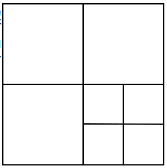
\includegraphics[trim=1.5 0 0 0, height=3.5cm,clip]{carto/4dtree.png}
		\caption{四个区域搜索空间}
	\end{figure}
\end{columns}

\end{frame}

\begin{comment}
\end{comment}
\begin{frame}
\frametitle{分支定界方法 \hfill 
\includegraphics[height=0.5cm]{logo.png}}
\begin{columns}
	\column{0.5\textwidth}
	\begin{itemize}
		\item 搜索树上的每个节点的上界可以通过下式计算得到:
		\vspace{0.2cm}
		\begin{equation}
			\begin{array}{lcr}
			 score(c)  & = &  \sum_{k=1}^K \mathop{max}\limits_{j \in \overline{\mathcal{V}_c}} M_{nearest(T_{\epsilon_j}, h_k)} \\
			 & \geq &\sum_{k=1}^K \mathop{max}\limits_{j \in \overline{\mathcal{W}_c}} M_{nearest(T_{\epsilon_j}, h_k)} \\
			 &\geq& \mathop{max}\limits_{j \in \overline{\mathcal{W}_c}} \sum_{k=1}^K M_{nearest(T_{\epsilon_j}, h_k)} 
			 \end{array}
		\end{equation}
		\item 如果对每一个节点都直接计算上界的话,将是一个很大的计算量.
		Cartographer采用一种类似图像金字塔的方法,{\color{red}预先计算出占用栅格地图在不同分支尺寸下的上界},
		在实际计算上界时只需要根据$c_h$查询对应尺度下的占用栅格即可获得节点的上界.右图是分支尺寸分别为1,4,16,64时的占用概率上界.
	\end{itemize}
	\column{0.4\textwidth}
	\begin{figure}[h]
		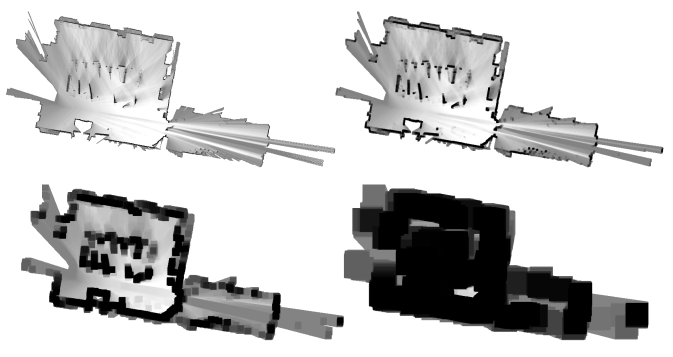
\includegraphics[trim=0 0 0 0, height=3.5cm,clip]{carto/precomputed_grid.png}
		\caption{分支尺寸分别为1/4/16/64时的占用概率上界}
	\end{figure}
\end{columns}
\end{frame}

\begin{comment}
\end{comment}
\begin{frame}
\frametitle{分支定界方法 \hfill 
\includegraphics[height=0.5cm]{logo.png}}
\begin{columns}
	%\column{0.1\textwidth}
	\column{0.7\textwidth}
	\begin{itemize}
		\item 我们称这个图为预算图,对于第$h$层的节点,在预算图中$x,y$的占用上界可以表示成下式,即以考察点$x,y$为中心,
		尺寸为$2^h \times 2^h$的窗口内栅格的最高占用概率为上界.
		\begin{equation}
			M_{precomp}^h(x,y) = \mathop{max}\limits_{
			\begin{matrix}
			x^\prime \in [x, x+r(2^h-1)]\\
			y^\prime \in [y, y+r(2^h-1)] 
			\end{matrix}}
			M_{nearest}(x^\prime, y^\prime)
		\end{equation}
		\vspace{0.2cm}
		\item 节点c的上界可以直接查表得到:
		\begin{equation}
			score(c) = \sum_{k=1}^K M_{precomp}^{c_h}(T_\epsilon h_k)
		\end{equation}
		\vspace{0.2cm}
		\item 整个闭环检测的业务逻辑是:根据当前的子图构建一个占用栅格地图,然后为该地图计算预算图,
		接着通过深度优先的分支定界搜索算法估计机器人的位姿,最后建立机器人位姿与子图之间的约束关系.
	\end{itemize}
%	\column{0.1\textwidth}

\end{columns}
\end{frame}


\begin{comment}
\end{comment}
\begin{frame}
\frametitle{分支定界方法 \hfill 
\includegraphics[height=0.5cm]{logo.png}}
\begin{columns}
	\column{0.3\textwidth}
	\begin{itemize}
		\item 把全部可行解空间反复分割为越来越小的子集,称为{\color{red}分支}.
		\item 对每个子集内的解集计算一个目标下界(对于最小值问题),称为{\color{red}定界}.
		\item 在每次分支后,凡是界限超出已知可行解集目标值的那些子集不再进一步分支,这样,许多子集可不予考虑,这称为{\color{red}减枝}.
		\item 分支定界法中,通过分支/定界/剪枝操作,使我们仅在一部分可行解中寻找最优解,而不是全部穷举出来在寻找,求解效率更高.
		%\vspace{0.3cm}
	\end{itemize}
	\column{0.7\textwidth}
	以整数规划为例,首先规定求解的整数规划问题为A,相应的线性规划问题为B(松弛问题).
	\begin{enumerate}
		\item 对问题B进行求解:
		\begin{enumerate}
			\item 若B无可行解,则A也无可行解,停止计算.
			\item 若B有最优解,且符合整数条件,该最优解为A的最优解,停止计算.
			\item 若B有最优解,但不符合整数条件,计它的目标函数值为$z^*$作为最优解的{\color{red}下界}.
		\end{enumerate}
%		\vspace{0.5cm}
		\item 找出问题A的一个可行解,其目标函数值作为最优解的{\color{red}上界}.
		\item 迭代:
		\begin{enumerate}
			\item 分支,在B中的最优解中人选一个不符合整数条件的变量$x_j$,其值为$b_j$,构造两个约束条件,$x_j \leq [b_j], x_j \geq [b_j] + 1$,分别加入到问题B中,形成两个子问题B1和B2.不考虑整数条件求解这两个子问题.
			\item 定界, 对每个后续问题表明其求解结果,与其他问题进行比较,将最优目标函数值最小者(不包括问题B)作为新的下界,
			在已符合整数条件的各分支中,找出目标函数值最小者作为新的上界.
			\item 剪枝,将目标函数不在下界和上界中的分支剪去.
			\item 重复123,直到得到最优解.
		\end{enumerate}
	\end{enumerate}

\end{columns}
\end{frame}

\begin{comment}
\end{comment}
\begin{frame}
\frametitle{分支定界方法 \hfill 
\includegraphics[height=0.5cm]{logo.png}}
\begin{columns}
	\column{0.6\textwidth}
	\begin{itemize}
		\item Cartographer使用类FastCorrelativeScanMatcher2D具体实现了深度优先的分支定界搜索算法,
		该算法能够高效地确定激光点云与子图的匹配度,估计采样点云时机器人相对于子图的位姿.
		为了能够高效的对搜索空间进行分割并计算上界,Cartographer还为每个子图计算了不同尺度下的占用概率,
		以后的搜索过程只需要简单的查表就可以完成.

	\end{itemize}

\end{columns}
\end{frame}

%%%%%%%%%%%%%%%%templete%%%%%%%%%%%%%%%%%%%%%
\begin{comment}
\end{comment}
\begin{frame}
\frametitle{分支定界方法 \hfill 
\includegraphics[height=0.5cm]{logo.png}}
\begin{columns}
	\column{0.5\textwidth}
	\begin{itemize}
		\item 
		\vspace{0.2cm}
		\item 
	\end{itemize}
	\column{0.5\textwidth}
	\begin{itemize}
		\item 
		\vspace{0.5cm}
		\item
	\end{itemize}
\end{columns}
\end{frame}

%%%%%%%%%%%%%%%%templete%%%%%%%%%%%%%%%%%%%%%

\begin{frame}[fragile]
\frametitle{branch and bound}
\end{frame}



\begin{frame}
\frametitle{branch and bound}
回环检测是一种匹配过程,即当获得新的scan时,再其附近一定范围内搜索最优匹配帧,若该最优匹配帧符合要求,则认为是一个回环.该匹配问题可以描述为以下式子.
\begin{equation}
\xi ^* = \mathop{argmax}\limits_{\xi \in W} \sum_{k=1}^K M_{nearest}(T_\xi h_k) \qquad (BBS)
\end{equation}

其中$W$是搜索空间,$M_{nearest}$是该点对应栅格点的$M$值.该式子可以理解为对于scan中的每一个光束映射到该地图中某个submap的某个laser scan上时的置信度和,置信度越高则认为越相似,我们需要在$W$空间中寻找出该置信度和最大的submap.

\end{frame}


% \section{IMU应用讲解计划}



\begin{frame}
  \frametitle{IMU应用讲解计划 \hfill 
\includegraphics[height=0.5cm]{00_logo.png}}
  \begin{columns}
    \column{0.1\textwidth}
    
    \column{0.6\textwidth}
    \begin{itemize}
      \item 第一期:旋转运动学 ;\quad IMU测量模型
      
      \item {\color{red}第二期:IMU误差模型 ;\quad IMU标定}

      \item 第三期:预积分(上)
      
      \item 第四期:预积分(下)


    \end{itemize}
    

    \column{0.1\textwidth}
  
  \end{columns}
  \end{frame}   
\section{旋转运动学}

\begin{comment}
\end{comment}
\begin{frame}
\frametitle{旋转运动学 \hfill 
\includegraphics[height=0.5cm]{00_logo.png}}
\begin{columns}
  \column{0.1\textwidth}
  
	\column{0.5\textwidth}
	\begin{itemize}
		\item 粒子在坐标系中$z=h$中的平面做圆周运动,坐标为:$r=(a\cos\theta, a \sin \theta, h)^T$,对坐标求导得:

    \begin{equation}
      \begin{split}
        \dot{r} &= (-a \dot{\theta} \sin \theta, a\dot{\theta}\cos\theta, 0)^T \\ 
          &= \begin{bmatrix}
        0 & -\dot{\theta} & 0 \\
        \dot{\theta} & 0 & 0 \\
        0 & 0 & 0 \\
      \end{bmatrix}
      \begin{bmatrix}
        a\cos\theta \\ a\sin\theta \\ h
      \end{bmatrix} \\
      &= w^\land r
      \end{split}
    \end{equation}

    其中,$w^\land$是一个反对称矩阵,$w = (0, 0, \dot{\theta})$, $\dot{\theta}$是角速度.

    % \item 对上式公式两边取模得:  
    
    % \begin{equation}
    %   |\dot{r}| = |w| |r| \sin \phi = a|\dot{\theta}|
    % \end{equation}


  \end{itemize}
  
  \column{0.3\textwidth}
	\begin{figure}[h]
		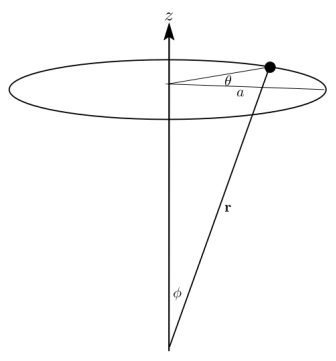
\includegraphics[trim=1.5 0 0 0, height=3.5cm,clip]{11_0.png}
		% \caption{四个区域搜索空间}
  \end{figure}
  
	\column{0.1\textwidth}

\end{columns}
\end{frame}

%%%%%%%%%%%%%%%%%%%%%%%%%%%%

\begin{frame}
  \frametitle{旋转运动学 \hfill 
\includegraphics[height=0.5cm]{00_logo.png}}
  \begin{columns}
    \column{0.1\textwidth}
    
    \column{0.8\textwidth}
    \begin{itemize}
      \item 旋转矩阵是一个行列式为1的正交矩阵.且每个列向量都是单位向量且相互正交,它的逆等于它的转置.
      % \item 旋转矩阵求导:
      % \begin{equation}
      %   \begin{split}
      %     \dot{R}(t)R(t)^T &= \phi(t)^\land \\
      %     \dot{R}(t) &= \phi(t)^\land R(t) \\
      %   \end{split}
      % \end{equation} 

      \item 旋转矩阵求导:
      \begin{equation}
        \begin{split}
          \dot{R}_{ib} &= \lim_{\Delta t \to 0} \frac{R_{ib} exp([w^b\Delta t]^\land) - R_{ib}}{\Delta t} \\
          &= \lim_{\Delta t \to 0} \frac{R_{ib} (exp([w^b\Delta t]^\land) - I)}{\Delta t} \\
          &\approx R_{ib} [w^b]^\land  \\
          & = [R_{ib}w^b]^\land R_{ib} \\
          & = [w^i]^\land R_{ib}
        \end{split}
      \end{equation} 

      \item 旋转矩阵求导2:
      \begin{equation}
        \begin{split}
          \dot{R}(t)R(t)^T &= \phi(t)^\land \\
          \dot{R}(t) &= \phi(t)^\land R(t) \\
        \end{split}
      \end{equation} 

    \end{itemize}


    % {\color{red}旋转矩阵是一个正交矩阵.它的行列式为1,且每个列向量都是单位向量且相互正交,它的逆等于它的转置.}
    
    \column{0.1\textwidth}
  
  \end{columns}
  \end{frame}   



%%%%%%%%%%%%%%%%%%%%%%%%%%%%

\begin{frame}
  \frametitle{旋转运动学 \hfill 
\includegraphics[height=0.5cm]{00_logo.png}}
  \begin{columns}
    \column{0.1\textwidth}
    \column{0.8\textwidth}
    更复杂一点的情况:一个旋转的水平光滑圆盘上,有一个光滑的小球,从圆心沿着半径向外运动.
    
    \begin{itemize}
      \item 从圆盘旋转坐标系来观察,小球轨迹如何?
      \item 从世界的坐标系来观察,小球轨迹如何?
      \item 科氏力,离心力,欧拉力?
      
    \end{itemize}

    \begin{figure}[h]
      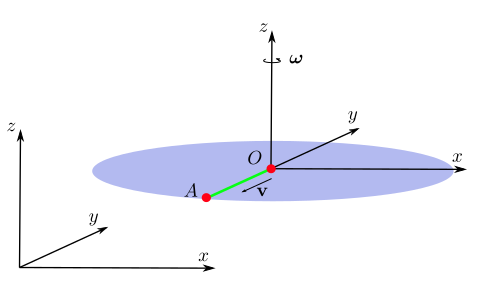
\includegraphics[trim=1.5 0 0 0, height=3.5cm,clip]{11_1.png}
      \qquad
      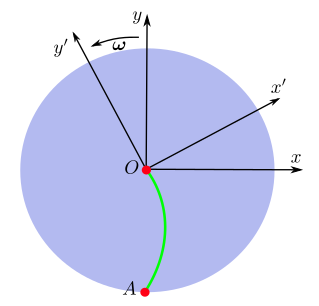
\includegraphics[trim=1.5 0 0 0, height=3.5cm,clip]{11_2.png}

      % \caption{四个区域搜索空间}
    \end{figure}
    \begin{figure}[h]
      % \caption{四个区域搜索空间}
    \end{figure}
    
    \column{0.1\textwidth}
  \end{columns}
  \end{frame}

%%%%%%%%%%%%%%%%%%%%%%%%%%%%

  \begin{frame}
    \frametitle{旋转运动学 \hfill 
\includegraphics[height=0.5cm]{00_logo.png}}
    \begin{columns}
      \column{0.1\textwidth}
      
      \column{0.5\textwidth}
      \begin{itemize}
        \item 质量块在body坐标系下的坐标为: $r^b = (x_1, x_2, x_3)^T$
        \item 忽略平移,只考虑旋转,旋转到惯性坐标系下:$r^i = R_{ib} r^b$
        \item 对时间求导:
    
        \begin{equation}
          \begin{split}
            \dot{r} &= R_{ib} \dot{r}^b + \dot{R}_{ib} r^b \\
            &= R_{ib} \dot{r}_b + R_{ib}[w^b]^\land r^b \\
            &= R_{ib} \dot{r}_b + [R_{ib}w^b]^\land R_{ib}r^b \\
            &= R_{ib} v^b + [w^i]^\land r^i \\
            &v = v^i + [w^i]^\land r^i  \Leftrightarrow
            v^i = v - [w^i]^\land r_i
          \end{split}
        \end{equation}
    
        其中,$w^i = R_{ib} w^b, v^i = R_{ib}v^b$, 表示body坐标系的角速度或线速度在I系下的表示.
    
    
      \end{itemize}
      
      \column{0.3\textwidth}
      \begin{figure}[h]
        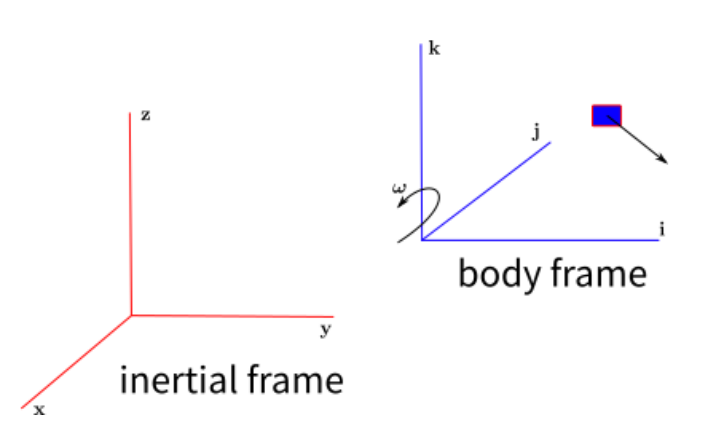
\includegraphics[trim=1.5 0 0 0, height=3.5cm,clip]{11_3.png}
        % \caption{四个区域搜索空间}
      \end{figure}
      
      \column{0.1\textwidth}
    
    \end{columns}
    \end{frame}  
  

   


  %%%%%%%%%%%%%%%%%%%%%%%%%%%%

\begin{frame}
  \frametitle{旋转运动学 \hfill 
\includegraphics[height=0.5cm]{00_logo.png}}
  \begin{columns}
    \column{0.1\textwidth}
    
    \column{0.8\textwidth}
    \begin{itemize}
      \item 对速度求导:
  
      \begin{equation}
        \begin{split}
          \ddot{r} &= R_{ib} \dot{v}^b + \dot{R}_{ib} v^b +  [w^i]^\land \dot{r}^i + [\dot{R}_{ib} w^b + R_{ib}\dot{w}^b]^\land r^i  \\ 
          &= R_{ib}\dot{v}^b + \dot{R}_{ib} v^b + [w^i]^\land \dot{r}^i +  [R_{ib}\dot{w}^b]^\land r^i  \\ 
          &= R_{ib} a^b + [w^i]^\land v^i + [w^i]^\land (v^i+[w^i]^\land r^i) + [\dot{w}^i]^\land r^i \\ 
          &= R_{ib} a^b + 2[w^i]^\land v^i + [w^i]^\land([w^i]^\land r^i) + [\dot{w}^i]^\land r^i \\
          \Rightarrow a^i &= a - \begin{matrix}
          \underbrace{2[w^i]^\land v^i}\\ Coriolis \ force
        \end{matrix} - \begin{matrix}
          \underbrace{[w^i]^\land([w^i]^\land r^i)}\\ centrifugal \ force
        \end{matrix} - \begin{matrix}
          \underbrace{[\dot{w}^i]^\land r^i}\\ Euler \ force 
        \end{matrix}
        \end{split}
      \end{equation}
  
      其中,$v^i = R_{ib}v^b, a^i = R_{ib}a^b$,表示物体在body下的速度或加速度在I系下的表示.

      
  
      {\color{red}在旋转坐标系下观察,运动的物体(运动方向和旋转轴不为同一个轴时)会受到科氏力的作用.}
    \end{itemize}
    
    \column{0.1\textwidth}
  
  \end{columns}
  \end{frame}      
  
  




\section{IMU测量模型}
\subsection{加速度计测量原理}
\subsection{陀螺仪的测量原理}

%%%%%%%%%%%%%%%%%%%%%%%%%%%%

\begin{frame}
  \frametitle{加速度计测量原理 \hfill \includegraphics[height=0.5cm]{00_logo.png}}
  \begin{columns}
    \column{0.1\textwidth}
    
    \column{0.5\textwidth}
    \begin{itemize}
      \item 其测量原理可以用一个质量块+弹簧+指示计来表示.
      \item 加速度计测量值$a_m$为弹簧拉力对应的加速度,
        \begin{equation}
          a_m = \frac{f}{m} = a - g
        \end{equation}
      
      其中,f为弹簧拉力, a为物体在惯性系下的加速度,g为重力加速度.
      
      \item 通过受力影响位移,位移影响电容大小,通过测量电流的方式获得$a_m$

    \end{itemize}

    \column{0.3\textwidth}
    \begin{figure}[h]
      \includegraphics[trim=1.5 0 0 0, height=3.5cm,clip]{12_0.png}
      % \caption{四个区域搜索空间}
    \end{figure}

    \column{0.1\textwidth}
  
  \end{columns}
  \end{frame}    


%%%%%%%%%%%%%%%%%%%%%%%%%%%%

\begin{frame}
  \frametitle{陀螺仪测量原理 \hfill \includegraphics[height=0.5cm]{00_logo.png}}
  \begin{columns}
    \column{0.1\textwidth}
    
    \column{0.5\textwidth}
    \begin{itemize}
      \item 陀螺仪主要用来测量物体的旋转角速度,按测量原理分有震动陀螺/光纤陀螺等.

      \item 一般采用震动陀螺原理,通过测量Coriolis force 来间接得到角速度.
      
      \item 一个主动运动轴 + 一个敏感轴

    \end{itemize}
    
    \column{0.3\textwidth}
    \begin{figure}[h]
      \includegraphics[trim=1.5 0 0 0, height=3.5cm,clip]{12_1.png}
      % \caption{四个区域搜索空间}
    \end{figure}

    \column{0.1\textwidth}
  
  \end{columns}
  \end{frame}    

%%%%%%%%%%%%%%%%%%%%%%%%%%%%

\begin{frame}
  \frametitle{音叉振动陀螺原理 \hfill \includegraphics[height=0.5cm]{00_logo.png}}
  \begin{columns}
    \column{0.1\textwidth}
    
    \column{0.8\textwidth}
    \begin{itemize}
      \item 音叉中间为旋转轴,音叉左右两个质量块,做方向相反的正弦运动,质量块受到的科氏力方向相反.
      \item 为什么要这么做?一个质量块行不行?

    \end{itemize}
    
    % \column{0.4\textwidth}
    \begin{figure}[h]
      \includegraphics[trim=1.5 0 0 0, height=3.5cm,clip]{12_2.png}
      \qquad
      \includegraphics[trim=1.5 0 0 0, height=3.5cm,clip]{12_3.png}
      % \caption{四个区域搜索空间}
    \end{figure}

    \column{0.1\textwidth}
  
  \end{columns}
  \end{frame}    

%%%%%%%%%%%%%%%%%%%%%%%%%%%%

\begin{frame}
  \frametitle{思考 \hfill \includegraphics[height=0.5cm]{00_logo.png}}
  \begin{columns}
    \column{0.1\textwidth}
    
    \column{0.8\textwidth}
    \begin{itemize}
      \item 实际上,两个质量块不可能完全一致,也就是说陀螺仪的测量会受到外部加速度的影响,即常称的G-sensitivity.
      
      \item 加速度计不需要考虑科氏力的影响吗?

    \end{itemize}
    

    \column{0.1\textwidth}
  
  \end{columns}
  \end{frame}    
\input{contents/22_IMU测量模型.tex}
% \section{IMU误差模型}
\section{近期IMU应用中的问题及解决}

%%%%%%%%%%%%%%%%%%%%%%%%%%%%

\begin{frame}[fragile]
  \frametitle{近期IMU应用中的问题及解决(一) \hfill \includegraphics[height=0.5cm]{00_logo.png}}
  \begin{columns}
    \column{0.1\textwidth}
    
    \column{0.8\textwidth}
    \begin{itemize}
      \item 问题一:同样是右手坐标系,不同的是$z$轴上的数值取反(原来重力大小为-9.8,需要改成9.8),有两种方式.

      \item 方式一:
      
      \begin{lstlisting}[frame=shadowbox]  
        // pentu_ig1.urdf
        <joint name="imu_link_joint" type="fixed">
          <parent link="base_footprint" />
          <child link="imu" />
          <origin xyz="0 0 0" rpy="3.14 0 0"/>
        </joint>
      \end{lstlisting}

      \begin{lstlisting}[frame=shadowbox]  
        // SensorBridge::HandleImuMessage()
        imu_data->angular_velocity = Eigen::Vector3d{imu_data->angular_velocity[0], 
            -imu_data->angular_velocity[1], -imu_data->angular_velocity[2]};
        imu_data->linear_acceleration = Eigen::Vector3d{imu_data->linear_acceleration[0],
            -imu_data->linear_acceleration[1], imu_data->linear_acceleration[2]};    
        ......    
        trajectory_builder_->AddSensorData( sensor_id,
            carto::sensor::ImuData{imu_data->time, imu_data->linear_acceleration,
                               imu_data->angular_velocity});
      \end{lstlisting}

    \end{itemize}
    
    % \column{0.3\textwidth}
    % \begin{figure}[h]
    %   \includegraphics[trim=1.5 0 0 0, height=3.5cm,clip]{12_1.png}
    %   % \caption{四个区域搜索空间}
    % \end{figure}

    \column{0.1\textwidth}
  
  \end{columns}
  \end{frame}   

  %%%%%%%%%%%%%%%%%%%%%%%%%%%%

\begin{frame}[fragile]
  \frametitle{近期IMU应用中的问题及解决(一) \hfill \includegraphics[height=0.5cm]{00_logo.png}}
  \begin{columns}
    \column{0.1\textwidth}
    
    \column{0.8\textwidth}
    \begin{itemize}
      \item 方式二:
      
      \begin{lstlisting}[frame=shadowbox]  
        // pentu_ig1.urdf
        <joint name="imu_link_joint" type="fixed">
          <parent link="base_footprint" />
          <child link="imu" />
          <origin xyz="0 0 0" rpy="0 0 0"/>
        </joint>
      \end{lstlisting}

      \begin{lstlisting}[frame=shadowbox]  
        // SensorBridge::HandleImuMessage()
        imu_data->linear_acceleration[2] = -imu_data->linear_acceleration[2];    
        ......    
        trajectory_builder_->AddSensorData( sensor_id,
            carto::sensor::ImuData{imu_data->time, imu_data->linear_acceleration,
                               imu_data->angular_velocity});
      \end{lstlisting}

    \end{itemize}
    
    % \column{0.3\textwidth}
    % \begin{figure}[h]
    %   \includegraphics[trim=1.5 0 0 0, height=3.5cm,clip]{12_1.png}
    %   % \caption{四个区域搜索空间}
    % \end{figure}

    \column{0.1\textwidth}
  
  \end{columns}
  \end{frame}   


  %%%%%%%%%%%%%%%%%%%%%%%%%%%%

\begin{frame}[fragile]
  \frametitle{近期IMU应用中的问题及解决(二) \hfill \includegraphics[height=0.5cm]{00_logo.png}}
  \begin{columns}
    \column{0.1\textwidth}
    
    \column{0.8\textwidth}
    \begin{itemize}
      \item 问题二:IMU安装不是不水平的,base\_footprint到imu的静态TF的标定困难.解决方法是开发一个自动标定IMU的代码.

      
      \begin{lstlisting}[frame=shadowbox]  
        // pentu_ig1.urdf
        <joint name="imu_link_joint" type="fixed">
          <parent link="base_footprint" />
          <child link="imu" />
          <origin xyz="0 0 0" rpy="-0.00478014 -0.000399168 0"/>
        </joint>

      \end{lstlisting}

    \end{itemize}
    
    % \column{0.3\textwidth}
    % \begin{figure}[h]
    %   \includegraphics[trim=1.5 0 0 0, height=3.5cm,clip]{12_1.png}
    %   % \caption{四个区域搜索空间}
    % \end{figure}

    \column{0.1\textwidth}
  
  \end{columns}
  \end{frame}   

%%%%%%%%%%%%%%%%%%%%%%%%%%%%

\begin{frame}[fragile]
  \frametitle{近期IMU应用中的问题及解决(二) \hfill \includegraphics[height=0.5cm]{00_logo.png}}
  \begin{columns}
    \column{0.1\textwidth}
    
    \column{0.8\textwidth}
      \begin{lstlisting}[frame=shadowbox]  
        void ImuCallback(const sensor_msgs::ImuConstPtr& msg)
        {
          static int nums = 0;
          static Eigen::Vector3d calibr_sum;
          if(++nums > 500)
            return;
          if(nums <= 500)
          {
            std::unique_ptr<cartographer::sensor::ImuData> imu_data = ToImuData(msg);
            const Eigen::Quaterniond rotation = Eigen::Quaterniond::FromTwoVectors(
              imu_data->linear_acceleration, Eigen::Vector3d{0, 0, -9.8});  
            Eigen::Vector3d calibr = cartographer::transform::RotationQuaternionToAngleAxisVector(rotation);
            calibr_sum += calibr;
          }
          if(nums == 500)
              std::cout << "[rpy:]" << calibr_sum / 500 << std::endl;
        }
      \end{lstlisting}

    
    % \column{0.3\textwidth}
    % \begin{figure}[h]
    %   \includegraphics[trim=1.5 0 0 0, height=3.5cm,clip]{12_1.png}
    %   % \caption{四个区域搜索空间}
    % \end{figure}

    \column{0.1\textwidth}
  
  \end{columns}
  \end{frame}   




% 
\section{低成本导航方案}

\begin{comment}
\end{comment}
\begin{frame}
\frametitle{建图 \hfill \includegraphics[height=0.5cm]{logo.png}}
\begin{columns}
	\column{0.5\textwidth}
	\begin{itemize}
		\item 前端:使用最近一段时间传感器数据进行子图构建,对算力的需求较小,但存在累积误差.
		\item 后端:引入闭环检测方法,通过对整个地图和历史轨迹的优化,解决累积误差的问题.由于数据量和计算量都很大,
		使用了分支定界的方式进行优化,一定程度上减少了算力的需求.
		\vspace{0.2cm}
		\item 
	\end{itemize}
	\column{0.5\textwidth}
	\begin{itemize}
		\item 滤波(RBPF)方法与图优化方法建图比较:
		\begin{itemize}
			\item RBPF方法一般需要大量的粒子来获取较好的建图效果,并且每个粒子都会包含地图信息,计算量会随场景增大成指数增长,从而不适用于大场景的建图.其次粒子重采样过程会引起粒子耗散问题.图优化方法不会随建图场景增大计算量呈指数递增问题,从而更适合大规模场景中的建图.
			\item RBPF方法无法有效消除累计误差问题,而图优化方法通过闭环检测能够有效消除运行过程中的累计误差.
		\end{itemize}
		\vspace{0.5cm}
		\item
	\end{itemize}
\end{columns}
\end{frame}

\begin{comment}
\end{comment}
\begin{frame}
\frametitle{costmap \hfill \includegraphics[height=0.5cm]{logo.png}}
\begin{columns}
	\column{0.5\textwidth}
	\begin{itemize}
		\item costmap为全局规划器和局部规划器提供代价地图.
		\vspace{0.2cm}
		\item costmap通过多个图层描述环境信息:
		\begin{itemize}
			\item 静态地图层(static map layer):描述的是导航的地图信息.
			\item 障碍物层(obstacle layer):记录了环境中的障碍物.
			\item 膨胀层(inflation layer):根据用户指定的参数和机器人的尺寸将障碍物的占用删格区域放大一部分,以防止碰撞.
		\end{itemize}
	\end{itemize}
	\column{0.5\textwidth}
	\begin{itemize}
		\item 
		\vspace{0.5cm}
		\item
	\end{itemize}
\end{columns}
\end{frame}


\begin{comment}
\end{comment}
\begin{frame}
\frametitle{全局规划器 \hfill \includegraphics[height=0.5cm]{logo.png}}
\begin{columns}
	\column{0.5\textwidth}
	\begin{itemize}
		\item 采用基于启发式搜索策略A*搜索算法作为全局规划算法.启发式函数h(n)告诉A*从任何结点n到目标结点的最小代价评估值.(欧几里得距离,曼哈顿距离)
		\vspace{0.2cm}
		\item 实现过程:
		\begin{itemize}
			\item 从机器人的起始位置开始,逐步向周围节点扩展,直到目标点.
			\item 从目标点开始采样梯度下降方法搜索,直到起始位置.由此得到一条从起始位置到目标位置的最短路径.
		\end{itemize}	
	\epsilon
		\end{itemize}
	\column{0.5\textwidth}
	\begin{itemize}
		\item 局部规划的目标是跟踪全局规划器输出的全局规划,依据机器人的动态特性和周围障碍物的特征,生成控制机器人运动的速度指令.
		\vspace{0.5cm}
		\item 其实现过程为:
		\begin{itemize}
			\item 速度采样:在机器人的速度空间(线速度/角速度)中离散地采样.
			\item 轨迹生成:对每个样本,在机器人当前状态的基础上推演未来很短一段时间内的运动轨迹. 
			%根据速度采样的样本,机器人当前的状态,以及设置的很短一段时间,前向模拟出一条运动轨迹.
			\item 轨迹评分:根据发生碰撞的可能性/目标点的接近程度/全局轨迹的跟踪近似度/速度限制等多方面的评价指标对这些轨迹打分,
			选取得分最高的轨迹,将其对应的指令下发给底盘,控制机器人运动.
		\end{itemize}
	\end{itemize}
\end{columns}
\end{frame}




%%%%%%%%%%%%%%%%templete%%%%%%%%%%%%%%%%%%%%%
\begin{comment}
\end{comment}
\begin{frame}
\frametitle{分支定界方法 \hfill \includegraphics[height=0.5cm]{logo.png}}
\begin{columns}
	\column{0.5\textwidth}
	\begin{itemize}
		\item 
		\vspace{0.2cm}
		\item 
	\end{itemize}
	\column{0.5\textwidth}
	\begin{itemize}
		\item 
		\vspace{0.5cm}
		\item
	\end{itemize}
\end{columns}
\end{frame}

%%%%%%%%%%%%%%%%templete%%%%%%%%%%%%%%%%%%%%%


% \section{蒙特卡洛方法}

\begin{frame}
  \frametitle{基于模型的强化学习问题}
  \begin{itemize}
    \item 基于模型的强化学习问题,模型状态转移概率矩阵$P$是已知的,即MDP已知。
    \item 强化学习的两个问题定义为:
    \begin{enumerate}
      \item 预测问题---给定强化学习6个要素:状态集$S$,动作集$A$,模型状态转移概率矩阵$P$,即时奖励$R$,衰减因子$\gamma$,给定策略$\pi$。求解该策略的状态价值函数$v(\pi)$。
      \item 控制问题---给定强化学习5个要素:状态集$S$,动作集$A$,模型状态转移概率矩阵$P$,即时奖励$R$,衰减因子$\gamma$。求解最优的状态价值函数$v_*$和最优策略$\pi$。
    \end{enumerate}
    
  \end{itemize}
\end{frame}

\begin{frame}
  \frametitle{不基于模型的强化学习问题}
  \begin{itemize}
    \item 有更多强化学习问题,我们没有办法实现得到模型的状态转移概率矩阵$P$,这时如果仍然需要求解强化学习问题,那么这就是不基于模型的强化学习问题了。
    \item 它的两个问题一般定义为:
    \begin{enumerate}
      \item 预测问题---给定强化学习5个要素:状态集$S$,动作集$A$,即时奖励$R$,衰减因子$\gamma$,给定策略$\pi$。求解该策略的状态价值函数$v(\pi)$。
      \item 控制问题---给定强化学习5个要素:状态集$S$,动作集$A$,即时奖励$R$,衰减因子$\gamma$,探索率$\epsilon$。求解最优的状态价值函数$v_*$和最优策略$\pi$。
    \end{enumerate}
  \end{itemize}
\end{frame}

% \section{MCMC}
\begin{frame}
  \frametitle{MCMC概述}
  \begin{itemize}
    \item MCMC由两个MC组成,即蒙特卡罗方法(Monte Carlo Simulation,MC)和马尔科夫链(Markov Chain,MC)。MCMC是很多算法求解的基础。
  \end{itemize}
\end{frame}

\begin{frame}
  \frametitle{蒙特卡罗方法}
  \begin{itemize}
    \item MCMC由两个MC组成,即蒙特卡罗方法(Monte Carlo Simulation,MC)和马尔科夫链(Markov Chain,MC)。MCMC是很多算法求解的基础。
  \end{itemize}
\end{frame}

\begin{frame}
  \frametitle{概率分布采样}
  \begin{itemize}
    \item 对于常见的均匀分布Uniform(0,1)是容易得到采样样本的,一般通过线性同余发生器就可以很方便的生成(0,1)之间的伪随机数样本。
    \item 而其他常见的概率分布,无论是离散的分布还是连续的分布,它们的样本都可以通过Uniform(0,1)的样本转换而得。
          比如二维正态分布的样本$(Y1, Y2)$可以通过独立采样得到。Uniform(0,1)样本对$(X1, X2)$通过如下的式子转换而得:
          \begin{equation}
            \begin{cases}
              Y1 = \sqrt{-2\ln{X1}} \cos{(2\pi X2)} \\
              Y2 = \sqrt{-2\ln{X2}} \sin{(2\pi X2)}
            \end{cases}
          \end{equation}
    \item 其他一些常见的连续分布,比如t分布,F分布,Beta分布,Gamma分布等,都可以通过类似的方式从Uniform(0,1)得到的采样样本转化得到。
    \item 很多时候我们的$x$的概率分布并不是常见的分布,这意味着我们没法方便的得到这些非常见的概率分布的样本集。那这个问题怎么解决?
  \end{itemize}
\end{frame}

\begin{frame}
  \frametitle{接受-拒接采样}
  \begin{itemize}
    \item 对于概率分布不是常见的分布,一个可行的办法是采用接受-拒绝采样来得到该分布的样本。
    \item 假设存在一个分布$p(x)$太复杂在程序中没法直接采样,那么设定一个程序可采样的分布 $q(x)$ 比如高斯分布,然后按照一定的方法拒绝某些样本,
          以达到接近 $p(x)$ 分布的目的,其中$q(x)$叫做建议分布(Proposal Distribution)。
    \item 具体采用过程:设定一个方便采样的常用概率分布函数 $q(x)$,以及一个常量 $k$,使得 $p(x)$ 总在 $kq(x)$ 的下方。如下图。

  \end{itemize}

\end{frame}

\begin{frame}
  \frametitle{接受-拒接采样}
  \centering
  \begin{figure}
    
    \includegraphics[width=8cm,trim=0 0 0 0,clip]{mcmc/jiesoujujue.png}
    \caption{拒接-接受采样示意图}
  \end{figure}
  
  % \begin{itemize}
  %   \item  首先,采样得到𝑞(𝑥)的一个样本𝑧0,方法用概率分布采样。然后,从均匀分布$(0, kq(z_0))$中采样得到一个值$𝑢$。
  %          如果$u$落在了上图中的灰色区域,则拒绝这次抽样,否则接受这个样本$z_0$。
  %          重复以上过程得到n个接受的样本$z_0, z_1, z_{n-1}$则最后的蒙特卡罗方法求解结果为:$$\frac{1}{n}\sum_{i=0}^{n-1} \frac{f(z_i)}{p(z_i)}$$
  %          整个过程中,我们通过一系列的接受拒绝方法来达到用$q(x)$模拟$p(x)$概率分布的目的。
  % \end{itemize}
\end{frame}

\begin{frame}
  \frametitle{接受-拒接采样}
  % \includegraphics[width=5cm,trim=0 0 0 0,clip]{mcmc/jiesoujujue.png}
  \begin{itemize}
    \item  首先,采样得到𝑞(𝑥)的一个样本𝑧0,方法用概率分布采样。然后,从均匀分布$(0, kq(z_0))$中采样得到一个值$𝑢$。
           如果$u$落在了上图中的灰色区域,则拒绝这次抽样,否则接受这个样本$z_0$。
           重复以上过程得到n个接受的样本$z_0, z_1, ..., z_{n-1}$则最后的蒙特卡罗方法求解结果为:$$\frac{1}{n}\sum_{i=0}^{n-1} \frac{f(z_i)}{p(z_i)}$$
           整个过程中,我们通过一系列的接受拒绝方法来达到用$q(x)$模拟$p(x)$概率分布的目的。
  \end{itemize}
\end{frame}

\begin{frame}
  \frametitle{蒙特卡罗方法小结}
  \begin{itemize}
    \item 使用接受-拒绝采样,我们可以解决一些概率分布不是常见的分布的时候,得到其采样集并用蒙特卡罗方法求和的目的。
    但是接受-拒绝采样也只能部分满足我们的需求,在很多时候我们还是很难得到我们的概率分布的样本集。比如:
    \begin{enumerate}
      \item 对于一些二维分布$p(x, y)$,有时候我们只能得到条件分布$p(x|y)$和$p(y|x)$和,却很难得到二维分布$p(x,y)$一般形式,
      这时我们无法用接受-拒绝采样得到其样本集。
      \item 对于一些高维的复杂非常见分布$p(x_1, x_2, ..., x_n)$我们要找到一个合适的$q(x)$和$k$非常困难。
    \end{enumerate}
    \item 从上面可以看出,要想将蒙特卡罗方法作为一个通用的采样模拟求和的方法,必须解决如何方便得到各种复杂概率分布的对应的采样样本集的问题。
  \end{itemize}

\end{frame}
% \section{马尔科夫链}

\begin{frame}
  \frametitle{马尔科夫链概述}
  \begin{itemize}
    \item 马尔科夫链假设某一时刻状态转移的概率只依赖于它的前一个状态。
    \item 这样假设可以大大简化模型的复杂度,因此马尔科夫链在很多时间序列模型中得到广泛的应用,比如循环神经网络RNN,隐式马尔科夫模型HMM等,MCMC也需要它。
    \item 用精确的数学定义来描述,则假设我们的序列状态是$..., X_{t-2}, X_{t-1}, X_t, X_{t+1}, X_{t+2},...$,
    那么我们的在时刻$t+1$的状态的条件概率仅仅依赖于时刻$t$,即:
    $$P(X_{t+1}|...,X_{t-2},X_{t-1},X_t) = P(X_{t+1}|X_t)$$
    \item 既然某一时刻状态转移的概率只依赖于它的前一个状态,那么我们只要能求出系统中任意两个状态之间的转换概率,这个马尔科夫链的模型就定了。
    我们来看看下图这个马尔科夫链模型的具体的例子(来源于维基百科)。
  \end{itemize}
\end{frame}

\begin{frame}
  \frametitle{马尔科夫链概述}
  \begin{figure}
    \includegraphics[trim=0 0 0 0,clip,height=5cm]{mcmc/niuxiongshi.png}
    \caption{马尔科夫链是表示股市模型}
  \end{figure}
\end{frame}

\begin{frame}
  \frametitle{马尔科夫链概述}
  \begin{itemize}
    \item 这个马尔科夫链是表示股市模型的,共有三种状态:牛市(Bull market), 熊市(Bear market)和横盘(Stagnant market)。
    \item 每一个状态都以一定的概率转化到下一个状态。比如,牛市以0.025的概率转化到横盘的状态。
    这个状态概率转化图可以用矩阵的形式表示。如果我们定义矩阵阵$P$某一位置$P(i,j)$的值为$P(j|i)$,即从状态$i$转化到状态$j$的概率,
    并定义牛市为状态0, 熊市为状态1, 横盘为状态2。这样我们得到了马尔科夫链模型的状态转移矩阵为:
    \begin{equation*}
      P = 
      \begin{pmatrix}
        0.9 & 0.075 & 0.025 \\
        0.15 & 0.8 & 0.05  \\
        0.25 & 0.25 & 0.5 \\
      \end{pmatrix}
    \end{equation*}
  \end{itemize}
\end{frame}

\begin{frame}
  \frametitle{马尔科夫链模型状态转移矩阵的性质}
  \begin{itemize}
    \item 马尔科夫链模型的状态转移矩阵收敛到的稳定概率分布与初始状态概率分布无关。
    这是一个非常好的性质,也就是说,如果我们得到了这个稳定概率分布对应的马尔科夫链模型的状态转移矩阵,
    则我们可以用任意的概率分布样本开始,带入马尔科夫链模型的状态转移矩阵,这样经过一些序列的转换,最终就可以得到符合对应稳定概率分布的样本。
    \item 如果一个非周期的马尔科夫链有状态转移矩阵$P$, 并且它的任何两个状态是连通的,那么$\lim_{n \to \infty} P_{ij}^n$与$i$无关,我们有:
  \end{itemize}

\end{frame}

\begin{frame}
  \frametitle{}
  \begin{enumerate}
    \item $$\lim_{n \to \infty} P_{ij}^n = \pi(j)$$
    \item $$\lim_{n \to \infty} P_{ij}^n = 
    \begin{pmatrix}
      \pi(1) &\pi(2)&...&\pi(3)&...\\
      \pi(1) &\pi(2)&...&\pi(3)&...\\
      ... &...&...&...&...\\
      \pi(1) &\pi(2)&...&\pi(3)&...\\
      ... &...&...&...&...\\
    \end{pmatrix}
    $$
    \item 
  \end{enumerate}
  
\end{frame}

\begin{frame}
  \frametitle{}
  \begin{enumerate}
    \item $$\pi(j) = \sum_{i=0}^\infty \pi(i)P_{ij}$$
    \item $\pi$ 是方程$\pi P = \pi$的唯一非负解,其中:$$\pi = [\pi(1), \pi(2),...,\pi(j), ...] \sum_{i=0}^\infty \pi(i) = 1$$
  \end{enumerate}
  
\end{frame}

\begin{frame}
  \frametitle{基于马尔科夫链采样}
  
\end{frame}








% \begin{frame}[plain]{}
%   \begin{center}
%     \begin{tikzpicture}
%       \node[above,xscale=1.2,yscale=1.2]{\Huge 欢迎批评指正!};
%     \end{tikzpicture}
%   \end{center}
% \end{frame}

\begin{frame}[plain]{}
  \begin{center}
    \begin{tikzpicture}
      \node[above,xscale=1.2,yscale=1.2]{\Huge {\color{red}{讨论一波嗨!!!}}};
    \end{tikzpicture}
  \end{center}
\end{frame}

% {\color{red}第一期:旋转运动学 ;\quad IMU测量模型}

\end{document}
